\documentclass[12pt,UTF8]{ctexbook}

% 导入设定
\input{../shared/settings}

% 封面
\title{\zihao{0} \bfseries 第六册}
\author{\zihao{2} \texttt{大青花鱼}}
% \date{\bfseries\today}
\date{}
% 正文
\begin{document}
\maketitle
\tableofcontents
\newpage

\chapter{向量函数的变化}

\section{平直空间中的向量函数}

我们学习过平面、立体空间中的变换。比如，平面上关于某条直线的对称变换，把平面中任一点映射到平面中另一点。空间中关于某个旋转轴的旋转变换，把空间中任一点映射到空间中另一点。空间中关于某平面的投影变换，把空间中任一点映射到该平面上的点。研究和工作生产实践中，我们也会遇到种种和平面、空间的点和向量有关的问题。

\begin{ex}
    % 物理中的向量场的例子
\end{ex}

数学上，我们用实系数平直空间中的映射来统一描述这些问题。给定平直空间$\mathbb{R}^m$、$\mathbb{R}^n$（其中$m,n$是正整数），我们把从$\mathbb{R}^m$到$\mathbb{R}^n$的映射称为$\mathbb{R}^m$到$\mathbb{R}^n$的向量函数。$m=n=1$时的向量函数就是实函数，$m=1$、$n=2$时的向量函数可以是实变复函数或描述平面曲线的实变向量函数，$m=n=2$时的向量函数可以是平面上的直变换和维直变换，$m=n=3$时的向量函数可以是立体空间中的直变换和维直变换。我们一般把$m=1,n>1$时的向量函数称为\textbf{实变向量函数}，把$m>1,n=1$时的向量函数称为\textbf{多元函数}，$m,n$都大于$1$时，称为\textbf{多元变换}或\textbf{多元映射}。

如何着手研究向量函数呢？首先来回顾一下，我们是怎么学习实函数的。我们研究实函数时候，首先学习最简单的函数：正比例函数。正比例函数$x\mapsto kx$把坐标轴进行放缩。另一个简单的函数是平移函数：$x \mapsto x + b$，它把坐标轴平移。这两个函数保持坐标轴的性质。它们结合起来，是一次函数。一次函数的图像是直线，它保持直线的性质。对于一般的函数，我们希望用这些简单函数来辅助理解它们的性质。

首先我们讨论函数的连续性。函数$f$在一点$a$连续，当且仅当$x$趋于$a$时，$f(x)$总趋于$f(a)$。这是函数的局部性质。更进一步，我们可以把某些函数在微小局部的样貌用一次函数来表示：
$$ f(x) \approx f(a) + \partial f(a) \cdot (x - a).$$
我们把这种展示称为实函数的\textbf{微直观}。

对于性质“更好”的函数，我们可以把这个表示方法拓展到多项式，乃至用无穷项的累加直接表示函数。另一方面，我们发现，这些一次函数的斜率，以某种方式累积起来，就能得到原来的函数。这就建立了微观与宏观的结合。

对于向量函数，我们也希望用类似的方法来研究。我们首先学习“最简单”的向量函数。它们的性质和正比例函数、一次函数类似，都保持坐标轴的性质，把点、直线、平面映射为点、直线、平面。具体来说，设有$\mathbb{R}^m$到$\mathbb{R}^n$的向量函数$h$，如果它满足以下条件：
\begin{enumerate}[label=\arabic*.]
    \item 保持平移操作：$\forall \,\,\mathbf{u}, \,\,\mathbf{v}$，$h(\mathbf{u} + \mathbf{v}) = f(\mathbf{u}) + h(\mathbf{v})$
    \item 保持放缩操作： $\forall \,\,k, \,\, \mathbf{u}$，$h(k\cdot \mathbf{u}) = k \cdot h(\mathbf{u})$
\end{enumerate}
就说$h$是\textbf{直变换}或\textbf{平直变换}。我们证明过平面和立体空间中的直变换保持坐标轴的性质，并且总把点、直线、平面映射为点、直线、平面。所有$\mathbb{R}^m$到$\mathbb{R}^n$的平直变换的集合记作$\mathcal{L}(\mathbb{R}^m, \,\,\mathbb{R}^n)$。

其他更复杂的向量函数的性质，我们希望用平直变换来辅助理解。这个研究方法与我们研究实函数时候的方法是一样的。

\section{向量函数的极限}

在第五册中，我们学习了有邻空间中函数在一点的极限概念。本节中，我们将聚焦于赋长平直空间中向量函数的极限性质，特别是经典空间 $\mathbb{R}^n$ 中的函数。与实函数相比，向量函数的极限概念既有相似之处，也有本质区别。我们首先回顾极限的严格定义，然后探究一些特有的性质。

\begin{df}{\textbf{向量函数在一点的极限}}
给定赋长平直空间 $\mathbb{R}^m$ 到 $\mathbb{R}^n$ 的映射 $f$。设 $f$ 在 $\mathbf{a}\in\mathbb{R}^m$ 附近有定义，如果对任何 $r>0$，都存在 $d>0$，使得只要 $\mathbf{x}$ 到 $\mathbf{a}$ 的距离小于 $d$，$f(\mathbf{x})$ 到某定点 $\boldsymbol{l}$ 的距离就小于 $r$，那么就说 $f$ 在 $\mathbf{a}$ 处有极限 $\boldsymbol{l}$。记作：
$$ \lian{\mathbf{x}\to \mathbf{a}} f(\mathbf{x}) = \boldsymbol{l}. $$
\end{df}

向量函数的极限定义与实函数的极限定义形式上相同。区别在于，我们使用了平直空间中的距离概念。对经典空间 $\mathbb{R}^n$，我们可以使用经典距离 $\ell_2$ 来描述"接近"关系。然而，由于 $\mathbb{R}^n$ 中各种模是等价的，无论选择哪种模定义距离，极限的结果都相同。

\begin{tm}{\textbf{向量函数极限的分量刻画}}
给定经典空间 $\mathbb{R}^m$ 到 $\mathbb{R}^n$ 的函数 $f$ 以及点 $\mathbf{a}\in\mathbb{R}^m$，设 $f$ 可写为：
$$ \forall \mathbf{x} \in \mathbb{R}^m, \quad f(\mathbf{x}) = (f_1(\mathbf{x}), f_2(\mathbf{x}), \ldots, f_n(\mathbf{x})), $$
其中 $f_1, f_2, \ldots, f_n$ 是从 $\mathbb{R}^m$ 到 $\mathbb{R}$ 的函数。则
$$ \lian{\mathbf{x}\to \mathbf{a}} f(\mathbf{x}) = \boldsymbol{l} = (l_1, l_2, \cdots, l_n) $$
当且仅当
$$ \forall 1 \leqslant i \leqslant n, \quad \lian{\mathbf{x}\to \mathbf{a}} f_i(\mathbf{x}) = l_i. $$
\end{tm}

\begin{proof}
考虑经典模 $\ell_2$，有
$$ \|f(\mathbf{x}) - \boldsymbol{l}\|_2 = \sqrt{\sum_{i=1}^n (f_i(\mathbf{x}) - l_i)^2}. $$
若 $\lian{\mathbf{x}\to \mathbf{a}} f(\mathbf{x}) = \boldsymbol{l}$，则对任意 $r>0$，存在 $d>0$，使得当 $\|\mathbf{x}-\mathbf{a}\|<d$ 时，
$$ \sqrt{\sum_{i=1}^n (f_i(\mathbf{x}) - l_i)^2} < r. $$
因此，对任意 $1 \leqslant i \leqslant n$，当 $\|\mathbf{x}-\mathbf{a}\|<d$ 时，
$$ |f_i(\mathbf{x}) - l_i| \leqslant \sqrt{\sum_{j=1}^n (f_j(\mathbf{x}) - l_j)^2} < r. $$
这说明 $\lian{\mathbf{x}\to \mathbf{a}} f_i(\mathbf{x}) = l_i$。

反之，若对任意 $1 \leqslant i \leqslant n$，$\lian{\mathbf{x}\to \mathbf{a}} f_i(\mathbf{x}) = l_i$，则对任意 $r>0$，对每个 $i$ 都存在 $d_i>0$，使得当 $\|\mathbf{x}-\mathbf{a}\|<d_i$ 时，
$$ |f_i(\mathbf{x}) - l_i| < \frac{r}{\sqrt{n}}. $$
取 $d = \min\{d_1, d_2, \cdots, d_n\}$，则当 $\|\mathbf{x}-\mathbf{a}\|<d$ 时，
$$ \sqrt{\sum_{i=1}^n (f_i(\mathbf{x}) - l_i)^2} < \sqrt{n \cdot \left(\frac{r}{\sqrt{n}}\right)^2} = r. $$
这说明 $\lian{\mathbf{x}\to \mathbf{a}} f(\mathbf{x}) = \boldsymbol{l}$。
\end{proof}

\begin{ex}
考虑二元函数 $f: \mathbb{R}^2 \to \mathbb{R}$：
$$ f(x, y) = \begin{cases}
\dfrac{xy}{x^2+y^2} & \text{若 } (x, y) \neq (0, 0), \\
0 & \text{若 } (x, y) = (0, 0).
\end{cases} $$
研究 $f$ 在 $(0, 0)$ 处的极限。

我们沿着不同路径趋近 $(0, 0)$。首先考虑沿 $x$ 轴趋近（即 $y=0$）：
$$ \lian{x\to 0} f(x, 0) = \lian{x\to 0} \frac{x\cdot 0}{x^2+0^2} = 0. $$
同样，沿 $y$ 轴趋近（即 $x=0$）：
$$ \lian{y\to 0} f(0, y) = \lian{y\to 0} \frac{0\cdot y}{0^2+y^2} = 0. $$
然而，沿着 $y=x$ 趋近：
$$ \lian{x\to 0} f(x, x) = \lian{x\to 0} \frac{x\cdot x}{x^2+x^2} = \lian{x\to 0} \frac{x^2}{2x^2} = \frac{1}{2}. $$
由于沿不同路径极限不同，$f$ 在 $(0, 0)$ 处不存在极限。
\end{ex}

\begin{sk}
\mbox{} \\
\indent 1. 为什么在一元函数中，我们只需考虑从左右两侧趋近，而在向量函数中需要考虑从更多方向趋近？这反映了什么本质区别？\\
\indent 2. 能否找到一个二元函数，它在原点沿任何直线趋近时极限都相同，但在原点处整体极限不存在？尝试构造一个例子。
\end{sk}

在研究向量函数极限时，我们会遇到累次极限的概念。对二元函数 $f(x, y)$，考虑先让 $x$ 趋近 $a$，再让 $y$ 趋近 $b$，或者相反次序。两种次序得到的极限一样吗？

\begin{df}{\textbf{累次极限}}
给定二元函数 $f(x, y)$ 在点 $(a, b)$ 附近有定义。若对每个足够接近 $b$ 的 $y$，$\lian{x\to a} f(x, y)$ 存在，且 $\lian{y\to b} \left(\lian{x\to a} f(x, y)\right)$ 也存在，则称
$$ \lian{y\to b} \left(\lian{x\to a} f(x, y)\right) $$
为函数 $f$ 在 $(a, b)$ 处的累次极限（先 $x$ 后 $y$）。类似定义先 $y$ 后 $x$ 的累次极限。
\end{df}

累次极限与向量极限（即向量函数在一点的极限）有重要关系：

\begin{tm}{\textbf{向量极限与累次极限的关系}}
给定二元函数 $f: \mathbb{R}^2 \rightarrow \mathbb{R}$，若
$$ \lian{(x,y)\to (a,b)} f(x, y) = l $$
存在，且对每个足够接近 $b$ 的 $y$，$\lian{x\to a} f(x, y)$ 存在，且对每个足够接近 $a$ 的 $x$，$\lian{y\to b} f(x, y)$ 存在，那么两个累次极限都存在且等于 $l$：
\begin{align*}
\lian{y\to b} \left(\lian{x\to a} f(x, y)\right) &= l, \\
\lian{x\to a} \left(\lian{y\to b} f(x, y)\right) &= l.
\end{align*}
\end{tm}

\begin{proof}
设 $\lian{(x,y)\to (a,b)} f(x, y) = l$。对任意 $\varepsilon > 0$，存在 $\delta > 0$，使得当 $|x-a| < \delta$ 且 $|y-b| < \delta$ 时，
$$ |f(x, y) - l| < \varepsilon. $$
固定 $y$ 满足 $|y-b| < \delta$，则当 $|x-a| < \delta$ 时，$|f(x, y) - l| < \varepsilon$。这说明 $\lian{x\to a} f(x, y)$ 存在且等于某个值 $g(y)$，且 $|g(y) - l| \leq \varepsilon$。

由于 $\varepsilon$ 任意，$\lian{y\to b} g(y) = l$，即
$$ \lian{y\to b} \left(\lian{x\to a} f(x, y)\right) = l. $$
同理可证另一累次极限也等于 $l$。
\end{proof}

\begin{et}
考虑函数
$$ f(x, y) = \frac{x-y}{x+y} $$
在点 $(0, 0)$ 附近的行为。

首先，考察重极限 $\lian{(x,y)\to (0,0)} f(x, y)$。沿着 $x$ 轴（$y=0$）趋近：
$$ \lian{x\to 0} f(x, 0) = \lian{x\to 0} \frac{x}{x} = 1. $$
沿着 $y$ 轴（$x=0$）趋近：
$$ \lian{y\to 0} f(0, y) = \lian{y\to 0} \frac{-y}{y} = -1. $$
由于沿不同路径极限不同，向量极限不存在。

其次，考察累次极限。先计算 $\lian{x\to 0} f(x, y)$，对固定 $y \neq 0$：
$$ \lian{x\to 0} f(x, y) = \lian{x\to 0} \frac{x-y}{x+y} = \frac{-y}{y} = -1. $$
然后
$$ \lian{y\to 0} \left(\lian{x\to 0} f(x, y)\right) = \lian{y\to 0} (-1) = -1. $$

再计算 $\lian{y\to 0} f(x, y)$，对固定 $x \neq 0$：
$$ \lian{y\to 0} f(x, y) = \lian{y\to 0} \frac{x-y}{x+y} = \frac{x}{x} = 1. $$
然后
$$ \lian{x\to 0} \left(\lian{y\to 0} f(x, y)\right) = \lian{x\to 0} 1 = 1. $$

两个累次极限存在但不相等，且都不等于向量极限（向量极限不存在）。这与前面的定理并不矛盾，因为定理的前提条件是向量极限存在。
\end{et}

\begin{tm}{\textbf{极限的运算性质}}
设 $f, g$ 是从 $\mathbb{R}^m$ 到 $\mathbb{R}^n$ 的映射，$\mathbf{a} \in \mathbb{R}^m$。若
$$ \lian{\mathbf{x}\to \mathbf{a}} f(\mathbf{x}) = \boldsymbol{l}_1, \quad \lian{\mathbf{x}\to \mathbf{a}} g(\mathbf{x}) = \boldsymbol{l}_2,\quad \mbox{则：} $$

\begin{enumerate}[label=\arabic*.]
\item $\lian{\mathbf{x}\to \mathbf{a}} (f + g)(\mathbf{x}) = \boldsymbol{l}_1 + \boldsymbol{l}_2$，
\item $\lian{\mathbf{x}\to \mathbf{a}} (f - g)(\mathbf{x}) = \boldsymbol{l}_1 - \boldsymbol{l}_2$，
\item 若 $n=1$，$\lian{\mathbf{x}\to \mathbf{a}} (f \cdot g)(\mathbf{x}) = \boldsymbol{l}_1 \cdot \boldsymbol{l}_2$，
\item 若 $n=1$ 且 $\boldsymbol{l}_2 \neq 0$，$\lian{\mathbf{x}\to \mathbf{a}} \left(\displaystyle\frac{f}{g}\right)(\mathbf{x}) = \frac{\boldsymbol{l}_1}{\boldsymbol{l}_2}$。
\end{enumerate}
\end{tm}

\begin{proof}
由向量函数极限的分量刻画，可将问题转化为实函数极限的性质。这里以加法为例证明。

设 $f(\mathbf{x}) = (f_1(\mathbf{x}), f_2(\mathbf{x}), \cdots, f_n(\mathbf{x}))$，$g(\mathbf{x}) = (g_1(\mathbf{x}), g_2(\mathbf{x}), \cdots, g_n(\mathbf{x}))$，则
$$ (f + g)(\mathbf{x}) = (f_1(\mathbf{x}) + g_1(\mathbf{x}), f_2(\mathbf{x}) + g_2(\mathbf{x}), \cdots, f_n(\mathbf{x}) + g_n(\mathbf{x})). $$
由条件，对任意 $1 \leqslant i \leqslant n$，
$$ \lian{\mathbf{x}\to \mathbf{a}} f_i(\mathbf{x}) = l_{1,i}, \quad \lian{\mathbf{x}\to \mathbf{a}} g_i(\mathbf{x}) = l_{2,i}, $$
其中 $\boldsymbol{l}_1 = (l_{1,1}, \cdots, l_{1,n})$，$\boldsymbol{l}_2 = (l_{2,1}, \cdots, l_{2,n})$。

由实函数极限的加法性质，
$$ \forall \, 1 \leqslant i \leqslant n, \;\; \lian{\mathbf{x}\to \mathbf{a}} (f_i + g_i)(\mathbf{x}) = l_{1,i} + l_{2,i}. $$
因此，由向量函数极限的分量刻画，
$$ \lian{\mathbf{x}\to \mathbf{a}} (f + g)(\mathbf{x}) = (l_{1,1} + l_{2,1}, l_{1,2} + l_{2,2}, \cdots, l_{1,n} + l_{2,n}) = \boldsymbol{l}_1 + \boldsymbol{l}_2. $$

其他性质可类似证明。
\end{proof}

\begin{xt}
\mbox{} \\
\indent 1. 研究以下函数在指定点处的极限：
\begin{align*}
1).& \quad f(x, y) = \frac{x^2-y^2}{x^2+y^2}, \quad (0, 0) \\
2).& \quad g(x, y) = \frac{x^2y}{x^4+y^2}, \quad (0, 0) \\
3).& \quad h(x, y, z) = \frac{xyz}{x^2+y^2+z^2}, \quad (0, 0, 0)
\end{align*}
\indent 2. 研究以下累次极限：
\begin{align*}
1).& \quad \lian{y\to 0} \left(\lian{x\to 0} \frac{x-y}{x^2+y^2}\right), \quad \lian{x\to 0} \left(\lian{y\to 0} \frac{x-y}{x^2+y^2}\right) \\
2).& \quad \lian{y\to 0} \left(\lian{x\to 0} \frac{x^2-y^2}{x^2+y^2}\right), \quad \lian{x\to 0} \left(\lian{y\to 0} \frac{x^2-y^2}{x^2+y^2}\right) \\
3).& \quad \lian{y\to 0} \left(\lian{x\to 0} \sin{\frac{1}{x}} \cdot \frac{y}{x^2+y^2}\right), \quad \lian{x\to 0} \left(\lian{y\to 0} \sin{\frac{1}{x}} \cdot \frac{y}{x^2+y^2}\right)
\end{align*}
\indent 3. 证明：若 $f: \mathbb{R}^2 \to \mathbb{R}$ 满足
$$ \forall x, y \in \mathbb{R}, \quad |f(x, y)| \leq x^2 + y^2, $$
则 $\lian{(x,y)\to (0,0)} f(x, y) = 0$。
\end{xt}

向量函数的极限概念是研究向量函数局部性质的基础。在下一节中，我们将基于极限概念讨论向量函数的连续性质。与实函数相比，向量函数的极限具有更丰富的直观意义和更复杂的行为模式。理解这些差异，对我们建立正确的多维直觉至关重要。

一个值得思考的问题是：在工程和科学中，我们常会遇到各种多变量系统，如何用数学语言精确描述这些系统的行为？向量函数的极限理论正是为此提供了严格框架。当我们说一个物理量依赖于多个参数时，理解这些参数如何共同影响该物理量，本质上就是理解向量函数的极限和连续性质。这种理解，将为我们打开通向更复杂数学结构和应用领域的大门。

\section{向量函数的连续性质}
给定$\mathbb{R}^m$到$\mathbb{R}^n$的向量函数$f$，对于$\mathbb{R}^m$中某点$\mathbf{a}$，我们首先定义它在$\mathbf{a}$处连续的性质。这里我们用极限来定义连续：映射在一点的极限等于该点的值。

\begin{df}{\textbf{向量函数在一点连续}}
给定赋长平直空间$\mathbb{R}^m$到$\mathbb{R}^n$的函数$f$。设$f$在点$\mathbf{a}\in\mathbb{R}^m$附近有定义，如果
$$ \lian{\mathbf{x}\to \mathbf{a}} f(\mathbf{x}) = f(\mathbf{a}), $$
就说$f$在$\mathbf{a}$处连续。如果$f$在定义域内某开集$U$中每一点都连续，就说$f$在$U$上连续。
\end{df}

向量函数在一点连续，意味着当自变量从任意方向以任意方式趋近该点时，函数值都会趋近于该点的函数值。这种定义与实函数的连续性定义在形式上一致，但在多维空间中，这意味着更复杂的可能性。


\begin{tm}{\textbf{向量函数连续的分量刻画}}
给定经典空间$\mathbb{R}^m$到$\mathbb{R}^n$的函数$f$，设$f$可写为：
$$ \forall \mathbf{x} \in \mathbb{R}^m, \quad f(\mathbf{x}) = (f_1(\mathbf{x}), f_2(\mathbf{x}), \ldots, f_n(\mathbf{x})), $$
其中$f_1, f_2, \ldots, f_n$是从$\mathbb{R}^m$到$\mathbb{R}$的函数。则$f$在$\mathbf{a}$处连续当且仅当$f_1, f_2, \ldots, f_n$都在$\mathbf{a}$处连续。
\end{tm}

\begin{proof}
由向量函数极限的分量刻画定理，函数$f$在$\mathbf{a}$处连续当且仅当
$$ \lian{\mathbf{x}\to \mathbf{a}} f(\mathbf{x}) = f(\mathbf{a}), $$
即
$$ \lian{\mathbf{x}\to \mathbf{a}} (f_1(\mathbf{x}), f_2(\mathbf{x}), \ldots, f_n(\mathbf{x})) = (f_1(\mathbf{a}), f_2(\mathbf{a}), \ldots, f_n(\mathbf{a})). $$
同样根据极限的分量刻画，上式成立当且仅当
$$ \forall 1 \leqslant i \leqslant n, \quad \lian{\mathbf{x}\to \mathbf{a}} f_i(\mathbf{x}) = f_i(\mathbf{a}), $$
即$f_1, f_2, \ldots, f_n$都在$\mathbf{a}$处连续。
\end{proof}

\begin{ex}
考虑二元函数$f: \mathbb{R}^2 \to \mathbb{R}$：
$$ f(x, y) = \begin{cases}
\dfrac{xy}{x^2+y^2} & \text{若 } (x, y) \neq (0, 0), \\
0 & \text{若 } (x, y) = (0, 0).
\end{cases} $$
我们研究$f$在$(0, 0)$处的连续性。

首先，考虑沿$x$轴趋近$(0, 0)$（即$y=0$）：
$$ \lian{x\to 0} f(x, 0) = \lian{x\to 0} \frac{x \cdot 0}{x^2+0^2} = 0. $$
同样，沿$y$轴趋近$(0, 0)$（即$x=0$）：
$$ \lian{y\to 0} f(0, y) = \lian{y\to 0} \frac{0 \cdot y}{0^2+y^2} = 0. $$
然而，我们需要验证以任意方式趋近时极限是否为$0$。考虑使用极坐标变换：$x = r\cos\theta$, $y = r\sin\theta$，则
$$ f(x, y) = \frac{r^2\cos\theta\sin\theta}{r^2} = \cos\theta\sin\theta. $$
当$0<\theta <\displaystyle \frac{\pi}{2}$时，令$r \to 0$，则$(x,y) \to (0,0)$，然而$\cos\theta\sin\theta \neq 0$，这时：
$$ \lian{r\to 0} f(x, y)  = \lian{r\to 0} \cos\theta\sin\theta = \cos\theta\sin\theta \neq 0. $$
这说明$\lian{(x,y)\to(0,0)} f(x, y)$不一定存在，因此$f$在$(0, 0)$处不连续。
\end{ex}

\begin{sk}
\mbox{}\\
\indent 1. 考虑二元函数
$$ f(x, y) = \begin{cases}
\dfrac{xy}{x^2+y^2} & \text{若 } (x, y) \neq (0, 0), \\
0 & \text{若 } (x, y) = (0, 0).
\end{cases} $$
研究$f$在$(0, 0)$处的连续性。\\
\indent 2. 设想一个二元函数，它在原点沿任何直线趋近时极限都相同，但在原点处不连续。这样的函数存在吗？试构造一个例子。
\end{sk}

连续函数具有一些重要的基本性质。和实函数一样，连续向量函数的和、差、积、商（分母不为零）以及复合函数仍然是连续函数。我们下面给出一些重要结论。

\begin{tm}{\textbf{连续向量函数的运算性质}}
设$f, g$是$\mathbb{R}^m$到$\mathbb{R}^n$的连续映射，$h$是$\mathbb{R}^n$到$\mathbb{R}^p$的连续映射。
\begin{enumerate}[label=\arabic*.]
\item $f \pm g$在定义域上连续。
\item 如果$n=1$，则$fg$在定义域上连续。
\item 如果$n=1$且$g$在定义域上恒不为零，则$\frac{f}{g}$在定义域上连续。
\item 复合函数$h \circ f$在定义域上连续。
\end{enumerate}
\end{tm}

\begin{proof}
这些结论可以从向量函数极限的运算性质及连续函数的定义直接推导。以复合函数为例：

设$f$在$\mathbf{a}$处连续，$h$在$f(\mathbf{a})$处连续。我们需要证明$h \circ f$在$\mathbf{a}$处连续，即
$$ \lian{\mathbf{x}\to \mathbf{a}} h(f(\mathbf{x})) = h(f(\mathbf{a})). $$
因为$f$在$\mathbf{a}$处连续，所以$\lian{\mathbf{x}\to \mathbf{a}} f(\mathbf{x}) = f(\mathbf{a})$。
又因为$h$在$f(\mathbf{a})$处连续，由连续映射保持极限的性质，有
$$ \lian{\mathbf{y}\to f(\mathbf{a})} h(\mathbf{y}) = h(f(\mathbf{a})). $$
因此
$$ \lian{\mathbf{x}\to \mathbf{a}} h(f(\mathbf{x})) = h\left(\lian{\mathbf{x}\to \mathbf{a}} f(\mathbf{x})\right) = h(f(\mathbf{a})), $$
这就证明了$h \circ f$在$\mathbf{a}$处连续。

其他性质可类似证明。
\end{proof}

\begin{et}
考察函数$f: \mathbb{R}^2 \to \mathbb{R}$：
$$ f(x, y) = \sin(x^2 + y^2). $$
证明$f$在$\mathbb{R}^2$上连续。
\end{et}

\begin{so}
考虑两个函数$g: \mathbb{R}^2 \to \mathbb{R}$，$h: \mathbb{R} \to \mathbb{R}$：
$$ g(x, y) = x^2 + y^2, \quad h(t) = \sin t. $$
$g$是多项式函数，因此在$\mathbb{R}^2$上连续；$h$是正弦函数，在$\mathbb{R}$上连续。
而$f = h \circ g$，根据复合函数的连续性质，$f$在$\mathbb{R}^2$上连续。
\end{so}

对于实函数来说，连续意味着很多良好的性质，比如闭区间上的连续函数必然有界，且达到最大值和最小值，等等。对于向量函数来说，连续性质带来了什么呢？

连续函数把经典空间中的紧致集映射为紧致集。而$\mathbb{R}^m$、$\mathbb{R}^n$中的紧致集就是有界闭集。因此，有界闭集经过连续映射，仍然是有界闭集。当$n=1$时，紧致集的像是$\mathbb{R}$的有界闭子集，即紧致集上的连续多元函数必达到最大值和最小值。


\begin{tm}{\textbf{有界闭集上连续函数的性质}}
设$U \subseteq \mathbb{R}^m$是有界闭集，$f: U \to \mathbb{R}$是连续函数。则：
\begin{enumerate}[label=\arabic*.]
\item $f$在$U$上有界。
\item $f$在$U$上达到最大值和最小值，即存在$\mathbf{a}, \mathbf{b} \in U$，使得
$$ f(\mathbf{a}) = \supp{\mathbf{x} \in U} f(\mathbf{x}), \quad f(\mathbf{b}) = \inff{\mathbf{x} \in U} f(\mathbf{x}). $$
\item $f$在$U$上一致连续。
\end{enumerate}
\end{tm}

\begin{proof}
1). 由于$U$是有界闭集（紧致集），且$f$连续，根据第五册中的结论，$f(U)$也是$\mathbb{R}$中的有界闭集。因此$f$在$U$上有界。

2). 同理，$f(U)$是$\mathbb{R}$中的非空有界闭集，因此它有最大值和最小值。设$M = \max f(U)$，$m = \min f(U)$，则存在$\mathbf{a}, \mathbf{b} \in U$，使得$f(\mathbf{a}) = M$，$f(\mathbf{b}) = m$。

3). 由于$U$是紧致集，且$f$在$U$上连续，根据前面的结论，$f$在$U$上一致连续。
\end{proof}

% \begin{et}
% 设$f: \mathbb{R}^m \to \mathbb{R}$是连续函数，且当$\|\mathbf{x}\| \to +\infty$时，$f(\mathbf{x}) \to +\infty$。证明$f$在$\mathbb{R}^m$上取得最小值。
% \end{et}

% \begin{so}
% 由于$f(\mathbf{x}) \to +\infty$当$\|\mathbf{x}\| \to +\infty$，存在$R > 0$，使得当$\|\mathbf{x}\| > R$时，$f(\mathbf{x}) > f(\mathbf{0})$。

% 考虑闭球$B = \{\mathbf{x} \in \mathbb{R}^m \mid \|\mathbf{x}\| \leqslant R\}$，它是有界闭集。根据前面的定理，$f$在$B$上取得最小值，设最小值点为$\mathbf{x}_0 \in B$。

% 对于$\|\mathbf{x}\| > R$，我们有$f(\mathbf{x}) > f(\mathbf{0}) \geqslant \min_{B} f = f(\mathbf{x}_0)$。因此，$\mathbf{x}_0$也是$f$在$\mathbb{R}^m$上的最小值点。
% \end{so}

\begin{et}
    如果多元函数$f: \mathbb{R}^m\rightarrow\mathbb{R}$在自变量的模长趋于无穷大时总趋于无穷大，就说$f$是径向增函数。证明：在$\mathbb{R}^m$中连续的径向增函数总取到最小值。
\end{et}

\begin{so}
    首先把径向增函数的定义“翻译”成具体的语言：对任意实数$M$，总有$d>0$，使得只要$|\mathbf{x}| > d$，就有$f(\mathbf{x}) > M$。

    任取一点$\mathbf{a}\in\mathbb{R}^m$，考虑$M = f(\mathbf{a})$，存在$d>0$，使得只要$|\mathbf{x}| > d$，就有$f(x) > M$。考虑以原点为中心，半径为$d$的闭“球”：
    $$ \bigcirc_d = \bigcirc(\mathbf{0}, d) = \{\mathbf{x}\in\mathbb{R}^m \, | \, |\mathbf{x}| \leqslant d\}. $$
    它是有界闭集，因此是紧致集。而$f$在$\mathbb{R}^m$中连续，因此$\bigcirc_d$经过$f$映射的像$f(\bigcirc_d)$是$\mathbb{R}$的有界闭子集。这说明$f(\bigcirc_d)$有最小值$y_{\text{小}}$。
    $$ y_{\text{小}} = \underset{|\mathbf{x}|\leqslant d}{\text{小}} (f(\mathbf{x})). $$

    在$f(\bigcirc_d)$中取一个收敛到$y_{\text{小}}$的数列：$\{y_n\}_{n\in\mathbb{N}}$。按照像集的定义，存在$\bigcirc_d$中元素的序列$\{\mathbf{x}_n\}_{n\in\mathbb{N}}$，使得$f(\mathbf{x}_n) = y_n$。$\bigcirc_d$是紧致集，因此序列$\{\mathbf{x}_n\}$有收敛子列$\{\mathbf{x}_{\varphi(n)}\}$。设这个子列收敛到$x_{\text{小}}$。由于$\{\mathbf{x}_{\varphi(n)}\}$的像序列：$\{f(\mathbf{x}_{\varphi(n)})\} = \{y_{\varphi(n)}\}$是$\{y_n\}$的子列，因此趋于$y_{\text{小}}$。而$f$是连续函数，所以
    $$f(x_{\text{小}}) = \lian{n\to +\infty} f(\mathbf{x}_{\varphi(n)}) = y_{\text{小}}.$$

    按定义，$\forall |\mathbf{x}| > d$，$f(\mathbf{x}) > f(\mathbf{a})$，因此$\mathbf{a}\in\bigcirc_d$。于是按定义$y_{\text{小}}\leqslant f(\mathbf{a})$，因而$ |\mathbf{x}| > d$时$f(\mathbf{x}) > f(\mathbf{a})\geqslant y_{\text{小}}$。这说明$y_{\text{小}}$就是$f$在$\mathbb{R}^m$上的最小值，在$\mathbf{x}_{\text{小}}$处取到。
\end{so}

连续的径向增函数总能取到最小值，这个结论在讨论存在性问题时很有用，因为它能“非构造地”保证$x_{\text{小}}$和$y_{\text{小}}$存在。比如，在证明多项式函数在复数域中必然有根时，我们可以把复数域上的多项式函数视作$\mathbb{R}^2\rightarrow\mathbb{R}$的二元函数。若多项式$p$是首一多项式，可以证明复数域上的函数：$z\mapsto |p(z)|$是径向增函数。因此，根据以上定理，它总能取到最小值。这正是证明多项式函数在复数域中必然有根的第一步。

我们学习过一致连续的概念。
\begin{df}{\textbf{实函数一致连续}}
    设有定义在区间$I$上的函数$f$。如果对任意$r>0$，总有$d>0$，使得区间中距离小于$d$的任意两个数$x,y$，
    函数值的差都小于$r$，就说$f$在$I$上\textbf{一致连续}。
\end{df}

向量函数也有一致连续的说法。
\begin{df}{\textbf{向量函数一致连续}}
    设有函数$f:\mathbb{R}^m \rightarrow \mathbb{R}^n$。考虑集合$\mathbb{U}\subseteq \mathbb{R}^m$，如果对任意$r>0$，总有$d>0$，使得$U$中距离小于$d$的任意两个向量$\mathbf{x},\mathbf{y}$经过映射后，距离都小于$r$，就说$f$在$U$上\textbf{一致连续}。
\end{df}

我们知道，在闭区间上连续的实函数，必然一致连续。向量函数也有类似性质：
\begin{tm}
    紧致集上的连续向量函数一致连续。
\end{tm}

\begin{proof}
    证明思路与实函数的情形相同。给定$r>0$，根据连续性质，对$U$中任一点$\mathbf{x}$，总能找到$d_x > 0$，使得$|\mathbf{y} - \mathbf{x}| \leqslant 2d_x$时，总有$|f(\mathbf{y}) - f(\mathbf{x})| < \frac{r}{2}$。
    
    为了证明一致连续，我们要找一个统一的$d$，使得$U$中任意两点只要距离小于$d$，经$f$映射后距离就小于$r$。对于一般连续函数，$d_x$随着$\mathbf{x}$变化，并不统一。不过，现在$U$是紧致集，因此考虑开球集合$\{\bigcirc(\mathbf{x}, d_x) \, | \, \mathbf{x} \in U \}$，它是$U$的开覆盖。因此根据紧致集定义，存在有限开子覆盖：
    $$U\subseteq \bigcup_{i=1}^k \bigcirc(\mathbf{x}_i, d_{x_i}) .$$
    把这$k$个球的半径$d_{x_i}$中最小的半径记为$d_0$，那么$d_0$就是我们要找的$d$。

    对于$U$中任意两点$\mathbf{x},\mathbf{y}$，$\mathbf{x}$必然属于前述$k$个开球之一。不妨设$\mathbf{x}\in \bigcirc(\mathbf{x}_i, d_{x_i})$，那么按定义$|f(\mathbf{x}) - f(\mathbf{x}_i)| < \frac{r}{2}$。如果$|\mathbf{y} - \mathbf{x}| \leqslant d_0$，那么
    $$ |\mathbf{y} - \mathbf{x}_i| \leqslant |\mathbf{y} - \mathbf{x}| + |\mathbf{x} - \mathbf{x}_i| \leqslant d_0 + d_{x_i} \leqslant 2d_{x_i}. $$
    于是$|f(\mathbf{y}) - f(\mathbf{x}_i)| < \frac{r}{2}$。因此：
    $$ |f(\mathbf{y}) - f(\mathbf{x})| \leqslant |f(\mathbf{y}) - f(\mathbf{x}_i)| + |f(\mathbf{x}_i) - f(\mathbf{x})| < \frac{r}{2} + \frac{r}{2} = r.$$
    这就说明$f$在$U$上一致连续。
\end{proof}

直接讨论向量函数的连续和一致连续性质比较麻烦。我们引入一个更方便、更直观的概念：
\begin{df}{\textbf{自限性质}}
    给定向量函数$f$，如果有固定的数$k$，使得$f$定义域中任两点经过$f$映射后的距离不大于这两点距离的$k$倍，就说$f$是（$\boldsymbol{k}$\textbf{倍}）\textbf{自限}的。$k$称为$f$的\textbf{自限系数}。
\end{df}

自限性质的出发点是很自然的。连续，就是不要有局部的“跳跃”或过于剧烈的“波动”。而自限性质用自变量的变化来约束映射后的变化量，简单来说，就是约束变率的绝对值不得超过$k$。直观来说，$k$倍自限就说明映射在局部“斜率”不超过$k$，不如斜率为$k$的直线或直映射那么“陡峭”。

\begin{tm}
    自限的向量函数必然一致连续（因而连续）。
\end{tm}

\begin{proof}
    设向量函数$f$自限，系数为$k$。对任意$r>0$，任意两点$\mathbf{x},\mathbf{y}$只要距离小于$\displaystyle\frac{r}{k}$，那么：
    $$ |f(\mathbf{x}) - f(\mathbf{y})| \leqslant k\cdot |\mathbf{x} - \mathbf{y}| < k \cdot \frac{r}{k} = r. $$
    这说明$f$一致连续。
\end{proof}

下面来看一些基础的连续向量函数。通过自限性质来证明连续性质。

\begin{et}
    证明：
    \begin{enumerate}[label=\arabic*.]
        \item $\mathbb{R}^m$上的模映射是连续映射。
        \item $\mathbb{R}^m \rightarrow \mathbb{R}^n$的平直变换在经典邻则下是连续映射。
        \item $\mathbb{R}^m$上的整式映射在经典邻则下是连续映射。
        \item $\mathbb{R}^m$上到定点的距离映射是连续映射。
        \item $\mathbb{R}^m$上到紧致集的距离映射是连续映射。
    \end{enumerate}
\end{et}

\begin{so}
    1). 把向量映射到其模长的映射是$1$倍自限的，因此连续。

    2). 首先证明：如果有常数$A$使得$\forall \mathbf{x}$，$|f(\mathbf{x})|\leqslant A|\mathbf{x}|$，那么平直变换$f$是连续映射。

    根据平直变换的基本性质：
    $$ \forall \mathbf{x}, \mathbf{y}, \quad |f(\mathbf{x}) - f(\mathbf{y})| = |f(\mathbf{x} - \mathbf{y})| \leqslant A|\mathbf{x} - \mathbf{y}|.$$
    这说明平直变换$f$是$A$倍自限的，因此连续。

    再证明：对任意$\mathbb{R}^m \rightarrow \mathbb{R}^n$的平直变换，这样的常数$A$总存在。

    我们知道平直变换$f$的值由一组基底上的值确定。给定基底$B = (\mathbf{e}_1, \cdots, \mathbf{e}_m)$，记$f$在基底上的值为：
    $$ \forall 1\leqslant i\leqslant m, \quad f(\mathbf{e}_i) = \mathbf{v}_i\in\mathbb{R}^n.$$
    那么对任意$\mathbf{x} = x_1\mathbf{e}_1 + \cdots + x_m\mathbf{e}_m\in\mathbb{R}^m$，有：
    \begin{align*}
        |f(\mathbf{x})| &= \left|f\left(\sum_{i=1}^m x_i \mathbf{e}_i\right)\right| = \left|\sum_{i=1}^m x_i f\left(\mathbf{e}_i\right)\right| \\
        &\leqslant \sum_{i=1}^m |x_i| \left| f\left(\mathbf{e}_i\right)\right| = \sum_{i=1}^m |x_i|\cdot |\mathbf{v}_i| \\
        &\leqslant A \sum_{i=1}^m |x_i| = A\|\mathbf{x}\|_1
    \end{align*}
    其中$A$是所有$|\mathbf{v}_i|$中最大者，$\|\cdot\|_1$是出发空间$\mathbb{R}^m $上的一次模$\ell_1$。$\mathbb{R}^m $中的经典邻则对应二次模$\ell_2$，而我们知道$\ell_1$和$\ell_2$等价。于是有常数$B$使得
    $$ \forall \mathbf{x}, \quad \|\mathbf{x}\|_1 \leqslant B\|\mathbf{x}\|_2. $$
    因此，常数$AB$使得：
    $$ \forall \mathbf{x}, \quad |f(\mathbf{x})| \leqslant A\|\mathbf{x}\|_1 \leqslant AB\|\mathbf{x}\|_2. $$
    这说明平直变换$f$在经典邻则下是连续映射。

    3). $\mathbb{R}^m$上的整式映射，指给定了基底$B = (\mathbf{e}_1, \cdots, \mathbf{e}_m)$后，把任意$\mathbf{x} = x_1\mathbf{e}_1 + \cdots + x_m\mathbf{e}_m\in\mathbb{R}^m$映射到关于分量$x_1, x_2, \cdots, x_m$的整式的映射。它是一种多元函数。

    要证明整式映射是连续映射，首先看最基本的一次式情形：
    $$ p_i: \quad \mathbf{x} = x_1\mathbf{e}_1 + \cdots + x_m\mathbf{e}_m \mapsto x_i. $$
    $p_i$是平直变换，因此是连续映射。对于更复杂的多项式映射，我们可以把问题放到局部来看。$m$元多项式$p$的形式如下：
    $$ p: \quad \mathbf{x} \mapsto \sum_{(i_1,i_2,\cdots, i_m)\in I_m} a_{i_1, i_2, \cdots, i_m} x_1^{i_1} x_2^{i_2}\cdots x_m^{i_m}.$$
    其中下标集$I_m$是$\mathbb{N}^m$的有限子集，表示多项式各项的下标。每一项的次数$s_i$是各个指数下标$i_j$的和：$s_i = \sum_{l=1}^m i_l$。

    对给定点$\mathbf{x}$，考虑$\mathbf{x}$的有界邻域$C$，记$M$为其上界：
    $$ \forall \mathbf{x}\in C, \quad \|\mathbf{x}\|_2 \leqslant M.$$
    于是，多项式函数中的每一项$x_1^{i_1} x_2^{i_2}\cdots x_m^{i_m}$，都可以这样限制其大小：
    $$ \left|x_1^{i_1} x_2^{i_2}\cdots x_m^{i_m}\right| = |x_j|\cdot |x_j|^{i_j-1} \cdot \prod_{l\neq j} \left|x_l^{i_l}\right| \leqslant |x_j| \cdot M^{i_j-1} \cdot\prod_{l\neq j} M^{i_l} = M^{s_i - 1} |x_j| . $$
    其中$j$是所有$i_l$中最大者对应的下标，$\prod_{l\neq j}$表示把下标不为$j$的项乘起来。上式结果说明，在有界邻域$C$里，多项式函数$p$的每一项有常数$A_{i_1, i_2, \cdots, i_m} = M^{s_i - 1}$使得：
    $$  \left|x_1^{i_1} x_2^{i_2}\cdots x_m^{i_m}\right| \leqslant A_{i_1, i_2, \cdots, i_m} |x_j| \leqslant A_{i_1, i_2, \cdots, i_m} \|\mathbf{x}\|_1 $$
    于是多项式函数$p$满足：
    \begin{align*}
        \forall \mathbf{x}, \quad |p(\mathbf{x})| &\leqslant \sum_{(i_1,i_2,\cdots, i_m)\in I_m} a_{i_1, i_2, \cdots, i_m}A_{i_1, i_2, \cdots, i_m}\|\mathbf{x}\|_1 = A\|\mathbf{x}\|_1 \leqslant AB\|\mathbf{x}\|_2.
    \end{align*}
    这说明对任意$\mathbf{x}$多项式函数$p$在$\mathbf{x}$的某个有界邻域里连续。但连续是局部性质，因此多项式函数$p$在定义域上总连续。

    4). 考虑定点$\mathbf{p}\in\mathbb{R}^m$，到$\mathbf{p}$的距离映射为：
    $$ \eth_{\mathbf{p}}: \quad \mathbf{x}\mapsto |\mathbf{x} - \mathbf{p}|.$$
    根据距离映射的基本性质，
    $$ \forall \mathbf{x}, \mathbf{y} \in \mathbb{R}^m, \quad |\eth_{\mathbf{p}}(\mathbf{x}) - \eth_{\mathbf{p}}(\mathbf{y})| =\big| |\mathbf{x} - \mathbf{p}| - |\mathbf{p} - \mathbf{y}| \big| \leqslant |(\mathbf{x} - \mathbf{p}) + (\mathbf{p} - \mathbf{y})| = |\mathbf{x} - \mathbf{y}|. $$
    这说明$\eth_{\mathbf{p}}$是$1$倍自限的，因此连续。

    5). 给定紧致集$U\in\mathbb{R}^m$，对给定的点$\mathbf{x}$，考虑$U$中点到$\mathbf{x}$的距离映射：
    $$ \eth_{\mathbf{x}}: \quad \mathbf{u}\mapsto |\mathbf{u} - \mathbf{x}|.$$
    $\eth_{\mathbf{x}}$是连续映射，因此在紧致集$U$上的像达到最小值。即有$\mathbf{u}_x\in U$使得：
    $$ |\mathbf{u}_x - \mathbf{x}| = \underset{\mathbf{u}\in U}{\text{小}} |\mathbf{u} - \mathbf{x}| .$$
    我们把$\mathbf{u}_x$叫做$\mathbf{x}$到$U$的垂足。以上最小值取决于$\mathbf{x}$，于是我们可以定义映射：
    \begin{align*}
        \eth_{U} : \mathbb{R}^m\; &\rightarrow \qquad \mathbb{R} \\
        \mathbf{x} \quad &\mapsto \underset{\mathbf{u}\in U}{\text{小}} |\mathbf{u} - \mathbf{x}|
    \end{align*}
    下面证明$\eth_{U}$连续。

    考虑任意两点$\mathbf{x}, \mathbf{y}$及任意$\mathbf{u}\in U$，按距离映射的定义总有：
    $$ |\mathbf{x} - \mathbf{u}| + |\mathbf{x} - \mathbf{y}| \geqslant |\mathbf{y} - \mathbf{u}|,$$
    所以，对于$\mathbf{u}_x \in U$也有：
    $$ |\mathbf{x} - \mathbf{u}_x| + |\mathbf{x} - \mathbf{y}| \geqslant |\mathbf{y} - \mathbf{u}_x|,$$
    考虑$\mathbf{u}_y$，按定义：
    $$ |\mathbf{x} - \mathbf{u}_x| + |\mathbf{x} - \mathbf{y}| \geqslant |\mathbf{y} - \mathbf{u}_x| \geqslant |\mathbf{y} - \mathbf{u}_y|,$$
    于是：
    $$ |\mathbf{x} - \mathbf{y}| \geqslant |\mathbf{y} - \mathbf{u}_y| - |\mathbf{x} - \mathbf{u}_x|. $$
    同理有：
    $$ |\mathbf{y} - \mathbf{x}| \geqslant |\mathbf{x} - \mathbf{u}_x| - |\mathbf{y} - \mathbf{u}_y|. $$
    于是：
    $$ |\mathbf{x} - \mathbf{y}| \geqslant \big||\mathbf{y} - \mathbf{u}_y| - |\mathbf{x} - \mathbf{u}_x|\big| = \left|\eth_{U}(\mathbf{x}) - \eth_{U}(\mathbf{y})\right|. $$
    这说明$\eth_{U}$是$1$倍自限的，因此连续。

\end{so}

\begin{sk}
    
\end{sk}

\begin{xt}
    \mbox{} \\
    \indent 1. 研究以下函数在指定点处的连续性：
    \begin{align*}
    1).& \quad f(x, y) = \frac{x^2-y^2}{x^2+y^2}, \quad (0, 0) \\
    2).& \quad g(x, y) = \frac{x^2y}{x^4+y^2}, \quad (0, 0) \\
    3).& \quad h(x, y, z) = \frac{xyz}{x^2+y^2+z^2}, \quad (0, 0, 0)
    \end{align*}
    \indent 2. 证明函数$f(x, y) = \sqrt{x^2+y^2}$在$\mathbb{R}^2$上连续。\\
    \indent 3. 证明函数$f(x, y) = x^3\sin(y) + y^3\cos(x)$在$\mathbb{R}^2$上一致连续。\\
    \indent 4. 设$U$是$\mathbb{R}^m$的有界闭子集。\\
    \indent 4.1 为何一般来说无法定义把$\mathbb{R}^m$的点$\mathbf{x}$映射到它到$U$的垂足的映射$p_U$？举一个反例。\\
    \indent 4.2. 如果$X\subseteq \mathbb{R}^m$满足：
    $$ \forall \mathbf{u}, \mathbf{v}\, \in X, \;\, \forall t\in[0;1], \quad t\mathbf{u} + (1 - t)\mathbf{v} \in X,$$
    就说$X$是$\mathbb{R}^m$里的\textbf{凸集}。举一个$\mathbb{R}^2$中的例子来直观理解凸集。\\
    \indent 如果$U$不仅是有界闭子集，还是凸集，我们希望证明$p_U$存在且连续。\\
    \indent 4.3. 给定$\mathbf{x}, \mathbf{y}\in \mathbb{R}^m$，证明以下不等式：
    $$ \frac{\phantom{0}|\mathbf{x}|^2}{2}  + \frac{\phantom{0}|\mathbf{y}|^2}{2}  \geqslant \left|\frac{\mathbf{x} + \mathbf{y}}{2}\right|^2. $$
    举一个$\mathbb{R}^2$中的例子来直观理解这个不等式。\\
    \indent 4.4. 证明：对于经典模映射$\ell_2$，我们可以定义上述的映射$p_U$。\\
    \indent 4.5. 给定$\mathbf{x}\in\mathbb{R}^m$，设$\mathbf{u}_x = p_U(\mathbf{x})$是它到$U$的垂足。证明，对$U$中任一点$p$，对于$\ell_2$对应的内积$\nji{\cdot}{\cdot}$，有以下不等式：
    $$ \nji{\mathbf{x} - \mathbf{u}_x}{\mathbf{u}_x - \mathbf{p}} \geqslant 0.$$
    给出上式的直观解释，并根据直观解释作出证明。\\
    \indent 4.6. 根据以上不等式，证明：
    $$ \forall \mathbf{x}, \mathbf{y} \in \mathbb{R}^m, \quad \nji{\mathbf{x} - \mathbf{y}}{p_U(\mathbf{x}) - p_U(\mathbf{y})} \geqslant |p_U(\mathbf{x}) - p_U(\mathbf{y})|^2. $$
    \indent 4.7. 使用内积不等式证明：
    $$ |p_U(\mathbf{x}) - p_U(\mathbf{y})| \leqslant |\mathbf{x} - \mathbf{y}|, $$
    并给出最终结论。
\end{xt}

% 4.4.关键是说明垂足的唯一性。如果$\mathbf{x}$到$U$有两个不同的垂足，考虑其中点。由于$U$是凸集，中点也在$U$里，且$\mathbf{x}$到中点的距离严格小于到两个垂足的距离。矛盾！

% 4.5.证明：$\forall t\in[0;1]$，$t\mathbf{u}_x + (1 - t)\mathbf{p}\in U$，因此：
% $$ \forall t\in[0;1],\quad |\mathbf{x} - \mathbf{u}_x|^2 \leqslant |\mathbf{x} - (t\mathbf{u}_x + (1 - t)\mathbf{p})|^2 $$
% 因此
% \begin{align*}
%     0 &\leqslant |\mathbf{x} - ((1 - t)\mathbf{u}_x + t\mathbf{p})|^2 - |\mathbf{x} - \mathbf{u}_x|^2 \\
%     &= |\mathbf{x} - \mathbf{u}_x + t(\mathbf{u}_x - \mathbf{p})|^2 - |\mathbf{x} - \mathbf{u}_x|^2 \\
%     &= |\mathbf{x} - \mathbf{u}_x|^2 + |\mathbf{u}_x - \mathbf{p}|^2 t^2 + 2t\nji{\mathbf{x} - \mathbf{u}}{\mathbf{u}_x - \mathbf{p}} - |\mathbf{x} - \mathbf{u}_x|^2\\
%     &= |\mathbf{u}_x - \mathbf{p}|^2 t^2 + 2t\nji{\mathbf{x} - \mathbf{u}_x}{\mathbf{u}_x - \mathbf{p}}
% \end{align*}
% 上式对于$\forall t\in[0;1]$成立。考察二次函数：
% $$ f: t\mapsto |\mathbf{u}_x - \mathbf{p}|^2 t^2 + 2\nji{\mathbf{x} - \mathbf{u}_x}{\mathbf{u}_x - \mathbf{p}}t. $$
% 二次函数的抛物线开口向上，$f(0)=0$。因此，$f$的最小值不大于$0$。如果对称轴在$x=0$右边，那么$f$在$0$处递减，因此必然在$[0;1]$上某处小于$0$。这说明要使得$f$在$[0;1]$上恒大于等于$0$，必然要使对称轴在$x=0$左边，也就是说，
% $$ \frac{\nji{\mathbf{x} - \mathbf{u}_x}{\mathbf{u}_x - \mathbf{p}}}{|\mathbf{u}_x - \mathbf{p}|^2} \geqslant 0 $$
% 于是得到结论。

% 4.6.证明：考虑两点$\mathbf{x}, \mathbf{y}$，记其到$U$的垂足分别为$\mathbf{u}_x, \mathbf{u}_y\in U$，根据4.5.结果有：
% \begin{align*}
%     \nji{\mathbf{x} - \mathbf{u}_x}{\mathbf{u}_x - \mathbf{u}_y} & \geqslant 0, \\
%     \nji{\mathbf{y} - \mathbf{u}_y}{\mathbf{u}_y - \mathbf{u}_x} & \geqslant 0, 
% \end{align*}
% 两边各自相加，得到：
% $$ \nji{\mathbf{x} - \mathbf{y} - (\mathbf{u}_x- \mathbf{u}_y)}{\mathbf{u}_x - \mathbf{u}_y} \geqslant 0 . $$
% 移项可得：
% $$ \nji{\mathbf{x} - \mathbf{y}}{\mathbf{u}_x - \mathbf{u}_y} \geqslant \nji{\mathbf{u}_x- \mathbf{u}_y}{\mathbf{u}_x - \mathbf{u}_y} = |\mathbf{u}_x - \mathbf{u}_y|^2. $$
% 4.7.
% 根据内积不等式，
% $$ \nji{\mathbf{x} - \mathbf{y}}{\mathbf{u}_x - \mathbf{u}_y} \leqslant |\mathbf{x} - \mathbf{y}|\cdot |\mathbf{u}_x - \mathbf{u}_y|, $$
% 因此：
% \begin{align*}
%     |\mathbf{x} - \mathbf{y}|\cdot |\mathbf{u}_x - \mathbf{u}_y| &\geqslant \nji{\mathbf{x} - \mathbf{y}}{\mathbf{u}_x - \mathbf{u}_y} \geqslant |\mathbf{u}_x - \mathbf{u}_y|^2 \\
%     |\mathbf{x} - \mathbf{y}| &\geqslant |\mathbf{u}_x - \mathbf{u}_y|
% \end{align*}
% 这说明$p_U$是$1$倍自限的，因此连续。

\section{二元函数的变化}

在一点$\mathbf{a}$处连续的向量函数$f$，在$\mathbf{a}$附近如何变化？和研究实函数一样，我们也希望找到一个平直变换$L$，使得$f$在$\mathbf{a}$附近有微直观：
$$ f(\mathbf{x}) \approx f(\mathbf{a}) + L (\mathbf{x} - \mathbf{a}). $$

这个$L$显然依赖于函数$f$和$\mathbf{a}$，我们将它记为
$$ L = \diff f (\mathbf{a}). $$
或者说，对给定的$f$，有这样的映射$\diff f$：
\begin{align*}
    \diff f:\quad \mathbb{R}^m &\rightarrow \mathcal{L}(\mathbb{R}^m, \,\,\mathbb{R}^n) \\
    \mathbf{a}\; &\mapsto \; L = \diff f (\mathbf{a})
\end{align*}
它把某些点$\mathbf{a}$映射到我们为这点找到的平直变换$L$。我们把映射$\diff f$叫做$f$的\textbf{微变映射}，把它在点$\mathbf{a}$处的取值\footnote{注意：微变映射在一点的取值是一个平直变换，而不是数，也不是向量。}叫做$f$在$\mathbf{a}$处的\textbf{微变换}。$f$在点$\mathbf{a}$的微变换存在，就说$f$在$\mathbf{a}$\textbf{可微}。

我们将$\diff f (\mathbf{a})$平移，得到在$\mathbf{a}$处的值为$f(\mathbf{a})$的维直变换。和实函数的微变一样，这应该是使用平直变换近似描述$f$在$\mathbf{a}$附近的行为的最好办法。也就是说，在$\mathbf{a}$附近，
$$ \forall \mathbf{x}, \; f(\mathbf{x}) - f(\mathbf{a}) - \diff f (\mathbf{a})(\mathbf{x} - \mathbf{a}) = \olim{\mathbf{x} - \mathbf{a}}. $$

对一般的$f$和$\mathbf{a}$，如何找到$\diff f (\mathbf{a})$呢？我们从简单的情况开始研究。

考虑把平面上的点映射到实数的二元函数：
$$ f : \mathbb{R}^2 \mapsto \mathbb{R}.$$
这类函数在实际问题中有着广泛的应用。比如，地形图上的海拔高度可以看作平面上一点的函数，温度分布可以看作平面上点的位置的函数。理解二元函数在一点附近的变化性质，对我们分析复杂现象至关重要。

二元函数$f$把平面上的点$\mathbf{x} = (x_1,\,\, x_2)$映射到实数$f(\mathbf{x})$。我们也将它简单地记作：
$$ (x_1, x_2) \mapsto f(x_1, x_2) \in \mathbb{R}.$$
直观上，二元函数可以想象为三维空间中的曲面。考虑装备了直角坐标系$Oxyz$的立体空间，把自变量$(x_1,\,\, x_2)$看平面$Oxy$的点的坐标，把函数值看作曲面在该点处的“高度”，也就是用空间中形同的点$(x_1, x_2, f(x_1, x_2))$的集合描述二元函数。作在平面上某一点$(\mathbf{a})$附近，如果有平直变换$L$，使得在$\mathbf{a}$附近，
$$ \forall \mathbf{x}, \; f(\mathbf{x}) - f(\mathbf{a}) - L(\mathbf{x} - \mathbf{a}) = \olim{\mathbf{x} - \mathbf{a}}, $$
就说$f$在$\mathbf{a}$处可微。如何理解这里的$\olim{\mathbf{x} - \mathbf{a}}$呢？按定义，应该有：
$$ \lian{\mathbf{x} \to \mathbf{a}} \frac{\left|f(\mathbf{x}) - f(\mathbf{a}) - L(\mathbf{x} - \mathbf{a})\right|}{\left|\mathbf{x} - \mathbf{a}\right|} = 0.$$
如何表示$\mathbf{x}$趋近于$\mathbf{a}$呢，我们使用平面上的经典距离$\ell_2$来描述。上面的极限就是说$\forall r > 0$，都有$d > 0$，使得只要$\sqrt{(x_1 - a_1)^2 + (x_2 - a_2)^2} < d$，就有：
$$ \frac{\left|f(\mathbf{x}) - f(\mathbf{a}) - L(\mathbf{x} - \mathbf{a})\right|}{\sqrt{(x_1 - a_1)^2 + (x_2 - a_2)^2}} < r. $$
其中$\mathbf{x} = (x_1, x_2)$，$\mathbf{a} = (a_1, a_2)$。要注意上式中分子和分母采用的距离不同。分子的距离是$\mathbb{R}$中的绝对值函数，分母的距离是$\mathbb{R}^2$中的经典距离$\ell_2$。

为了方便，我们还可以把$\mathbf{x} - \mathbf{a}$作为变量来讨论，记$\mathbf{h} = \mathbf{x} - \mathbf{a}$，那么$\mathbf{x} = \mathbf{a} + \mathbf{h}$。我们可以说，$f$在$\mathbf{a}$处可微，当且仅当
$$ \lian{\mathbf{h} \to \mathbf{0}} \frac{\left|f(\mathbf{a} + \mathbf{h}) - f(\mathbf{a}) - L(\mathbf{h})\right|}{\left|\mathbf{h}\right|} = 0.$$
即$\forall r > 0$，都有$d > 0$，使得只要$|h| = \sqrt{h_1^2 + h_2^2} < d$，就有：
$$  \frac{\left|f(\mathbf{a} + \mathbf{h}) - f(\mathbf{a}) - L(\mathbf{h})\right|}{\sqrt{h_1^2 + h_2^2\phantom{0}}} < r.$$

上式中的$L(\mathbf{h})$是一个实数。这个实数如何与$\mathbf{h}$相关呢？$L$如何选取呢？

我们先来看一种特殊情形：$\mathbf{h}$是某个特定方向上的向量，沿着该方向趋于$\mathbf{a}$。具体来说，给定单位长度的向量$\mathbf{v}$（$|\mathbf{v}| = 1$），令$\mathbf{h} = t\mathbf{v}$，其中$t\in\mathbb{R}$是系数，表示$h$的长度。固定方向$\mathbf{v}$不变而让$t$变动。根据平直变换的基本性质，$L(\mathbf{h}) = tL(\mathbf{v})$，而$L(\mathbf{v})\in\mathbb{R}$是固定的实数，于是当$t$趋于$0$时：
\begin{align*}
    \frac{\left|f(\mathbf{a} + \mathbf{h}) - f(\mathbf{a}) - L(\mathbf{h})\right|}{|\mathbf{h}|} &= \frac{\left|f(\mathbf{a} + t\mathbf{v}) - f(\mathbf{a}) - tL(\mathbf{v})\right|}{|t|\cdot|\mathbf{v}|} \\ 
    &= \frac{\left|f(\mathbf{a} + t\mathbf{v}) - f(\mathbf{a}) - tL(\mathbf{v})\right|}{|t|}
\end{align*}
这就把二元函数的问题转化归结为实函数的问题。考虑实函数：
$$ f_{\mathbf{v}} : \;t\mapsto f(\mathbf{a} + t\mathbf{v}) \in \mathbb{R}$$
% 的变率极限：
% $$ \frac{\left|f(\mathbf{a} + \mathbf{h}) - f(\mathbf{a}) - L(\mathbf{h})\right|}{|\mathbf{h}|} = \frac{\left|f_{\mathbf{v}}(t) - f_{\mathbf{v}}(0) - tL(\mathbf{v})\right|}{|t|} $$
$ f_{\mathbf{v}}$在$t=0$处的微变率存在，就是说有实数$l$，使得：
$$ \lian{t\to 0} \frac{f(\mathbf{a} + t\mathbf{v}) - f(\mathbf{a})}{t} = \lian{t\to 0} \frac{f_{\mathbf{v}}(t) - f_{\mathbf{v}}(0)}{t} = l, $$
而对于$f$来说，如果$f$在$\mathbf{a}$处可微，那么：
$$ \lian{t\to 0} \left|\frac{f(\mathbf{a} + t\mathbf{v}) - f(\mathbf{a})}{t} - L(\mathbf{v}) \right|= \lian{t\to 0} \frac{\left|f(\mathbf{a} + t\mathbf{v}) - f(\mathbf{a}) - tL(\mathbf{v})\right|}{|t|} = 0.$$
这说明
$$ \lian{t\to 0} \frac{f(\mathbf{a} + t\mathbf{v}) - f(\mathbf{a})}{t} = L(\mathbf{v}).$$
因此$l = L(\mathbf{v})$。

换句话说，如果$f$在$\mathbf{a}$处可微，那么对任意单位长度的向量$\mathbf{v}$，实函数$ f_{\mathbf{v}}$在$t=0$处都应该可微，而且微变率应该就是$L(\mathbf{v})$。也就是说，通过求出各个方向上实函数$ t\mapsto f(\mathbf{a} + t\mathbf{v})$在$t=0$处的微变率，我们就得到了平直变换$L$的全貌。

前面已经说过，我们可以把二元函数理解为装备了直角坐标系$Oxyz$的立体空间中的曲面。把$Oxy$平面看作自变量$\mathbf{x} = (x_1, x_2)$的取值平面，用$z$轴的分量来表示函数值$f(\mathbf{x})$。也就是说，点集：
$$\left\{(x_1, x_2, f(x_1, x_2)) \, \big| \, x_1, x_2 \in \mathbb{R} \right\}$$
就是$f$在立体空间的直观表示。我们可以把这样的点集称为$f$的曲面。$f$在一点取值的大小，直观上对应该点位置上曲面的“高度”。

考虑沿着$\mathbf{v}$方向且垂直于$Oxy$平面的竖直平面$\gamma_{\mathbf{v}}$：
$$\gamma_{\mathbf{v}} = \{\mathbf{a} + t\mathbf{v} + s\mathbf{e}_z \, | \, t, s \in \mathbb{R}\}$$
其中$\mathbf{e}_z$是直角坐标系$Oxyz$对应的基底中$z$轴方向的基向量。实函数$f_{\mathbf{v}}$可以理解为从点$\mathbf{a}$出发，用$\gamma_{\mathbf{v}}$截取$f$的曲面得到的平面曲线。$ f_{\mathbf{v}}$在$t=0$处的微变率就是平面曲线在$\mathbf{a}$处的切线斜率。

\begin{figure}[h] %this figure will be at the right
    \vspace{4pt}
    \flushleft
    
    \tdplotsetmaincoords{70}{110}
    \begin{tikzpicture}[tdplot_main_coords]

        \begin{axis}[
            width=10cm, height=10cm,
            xmin=0, xmax=2,  ymin=0, ymax=2,  zmin=0, zmax=1,
            view={110}{18},
            axis equal image,
            axis lines=box,
            grid=major,
            grid style={dashed,lightgray},
            xtick={0,0.5,...,2},
            ytick={0,0.5,...,2},
            ztick={0,0.25,...,1},
            axis line style={opacity=0},
            tick style={draw=none},
            ticklabel style={opacity=0},
            xlabel=\empty, ylabel=\empty, zlabel=\empty,]
        \end{axis}

        \begin{axis}[
            view={110}{18},
            axis equal image,
            width=10cm,
            height=10cm,
            xmin=0, xmax=2,ymin=0, ymax=2, zmin=0, zmax=1,
            samples=50,
            domain=0:2,
            y domain=0:2,
            axis lines=middle,
            xlabel=$x$, ylabel=$y$, zlabel=$z$,
            xlabel style={sloped like x axis},
            ylabel style={sloped like y axis},
            xtick={0,0.5,...,2},
            ytick={0,0.5,...,2},
            ztick={0,0.25,...,1},
            axis on top,
            grid=none,
        ]
            % --- 定义点 a 和方向向量 v ---
            \pgfmathsetmacro{\ax}{1.0}
            \pgfmathsetmacro{\ay}{1.0}
            \pgfmathsetmacro{\az}{0.4 * sin(deg(\ax) + 80) + 0.4 * sin(1.5 * deg(\ay) + 20) + 0.09 + 0.06 * \ax * \ay}
            
            \pgfmathsetmacro{\vx}{0.3846}
            \pgfmathsetmacro{\vy}{0.9231}
            
            % --- 定义函数 f(x,y) ---
            \pgfmathdeclarefunction{MyFunc}{2}{\pgfmathparse{0.4 * sin(deg(#1) + 80) + 0.4 * sin(1.5 * deg(#2) + 20) + 0.09 + 0.06 * #1 * #2}}
            
            % --- 绘制函数曲面 ---
            \addplot3[surf, colormap/autumn, opacity=0.5] {MyFunc(x, y)};
            % \addplot3[surf, opacity=0.5] {0};
            
            % --- 绘制点 a 和其在曲面上的投影 ---
            \fill[black] (\ax, \ay, 0) circle (2pt) node[below] {$\mathbf{a}$};
            \fill[black] (\ax, \ay, \az) circle (2pt) node[above right] {$f(\mathbf{a})$};
            \draw[thick, dashed] (\ax, \ay, 0) -- (\ax, \ay, \az);
            
            % --- 绘制平面 Γ_v (使用矩形表示) ---
            \addplot3+[domain=-1:0, samples=50, samples y=0, no marks, thick, teal] 
                ({\ax + \vx*3/4*x}, {\ay + \vy*3/4*x}, {0});
            \addplot3+[domain=0:1, samples=50, samples y=0, no marks, dashed, thick, teal] 
                ({\ax + \vx*3/4*x}, {\ay + \vy*3/4*x}, {0});
            \addplot3+[domain=0:1, samples=50, samples y=0, no marks, dashed, thick, teal] 
                ({\ax - \vx*3/4}, {\ay - \vy*3/4}, {x * MyFunc(\ax - \vx*3/4, \ay - \vy*3/4)});
            \addplot3+[domain=0:1, samples=50, samples y=0, no marks, dashed, thick, teal] 
                ({\ax + \vx*3/4}, {\ay + \vy*3/4}, {x * MyFunc(\ax + \vx*3/4, \ay + \vy*3/4)});
            
            % --- 绘制方向向量 v ---
            \draw[-Stealth, blue, thick] (\ax, \ay, 0) -- (\ax + \vx/2, \ay + \vy/2, 0) node[above right] {$\mathbf{v} = \left(\frac{5}{13},\frac{12}{13}\right)$};
            
            % --- 绘制平面 Γ_v 和曲面的交线 ---
            \addplot3[domain=-1.5:1.5, samples=50, samples y=0, no marks, thick, blue] 
                ({\ax + \vx/2*x}, {\ay + \vy/2*x}, {MyFunc(\ax + \vx/2*x, \ay + \vy/2*x)});
            
            % --- 绘制点 a 处的切线 ---
            \pgfmathsetmacro{\dfdx}{0.4 * cos(deg(\ax) + 80) + 0.06 * \ay}
            \pgfmathsetmacro{\dfdy}{0.6 * cos(1.5 * deg(\ay) + 20) + 0.06 * \ax}
            \pgfmathsetmacro{\tangentz}{\dfdx*(\vx/2) + \dfdy*(\vy/2)}
            
            \addplot3[domain=-0.8:0.8, samples=50, samples y=0, no marks, thick, Purple] 
                ({\ax + \vx/2*x}, {\ay + \vy/2*x}, {\az + \tangentz*x});
                
            \node[teal] at (0.0,0.0,0.5) [above right] {$\gamma_{\mathbf{v}}$};
        \end{axis}
            
    \end{tikzpicture}
    \caption*{$f$\texttt{的曲面上}$\mathbf{a}=(1,1)$\texttt{处沿}$\mathbf{v}= \left(\frac{5}{13},\frac{12}{13}\right)$\texttt{方向的切线}}
\end{figure}

我们把$ f_{\mathbf{v}}$在$t=0$处的微变率称为$\boldsymbol{f}$\textbf{沿}$\mathbf{v}$\textbf{方向的微变率}，简称\textbf{方向微变}，记作$\diff_{\mathbf{v}} f(\mathbf{a})$。如果$\mathbf{v}$是基向量$(1,0)$或$(0,1)$，就说它是$\boldsymbol{f}$\textbf{的首元（次元）微变率}，合称\textbf{偏微变率}。二元函数$f$在$\mathbf{a}$处的偏微变可以简记为$\partial_{x} f(\mathbf{a}), \partial_{y} f(\mathbf{a})$或$\partial_{1} f(\mathbf{a}), \partial_{2} f(\mathbf{a})$。

二元函数在一点可微，则它在这点的任何方向微变和偏微变都存在。从可微二元函数在一点的偏微变出发，我们可以求出函数在该点的微直观$L$。这是因为$L$作为平直变换，必然由它在平面基向量上的值完全确定。如果已知：
$$ L(\mathbf{e}_1) = \partial_{1} f(\mathbf{a}), \quad L(\mathbf{e}_2) = \partial_{2} f(\mathbf{a}), $$
那么对任意向量$\mathbf{h}$，$\mathbf{h}$可以唯一表示为平面基向量的直组合：
$$ \mathbf{h} = h_1 \mathbf{e}_1 + h_2 \mathbf{e}_2. $$
于是：
$$ L(\mathbf{h}) = L(h_1 \mathbf{e}_1 + h_2 \mathbf{e}_2) = h_1 L(\mathbf{e}_1) + h_2 L(\mathbf{e}_2) = h_1 \partial_{1} f(\mathbf{a}) + h_2 \partial_{2} f(\mathbf{a}) . $$
也就是说，$f$在$\mathbf{a}$附近可以写成：
$$ \forall h_1, h_2\in \mathbb{R}, \; f(\mathbf{a} + h_1 \mathbf{e}_1 + h_2 \mathbf{e}_2) \approx f(\mathbf{a}) + h_1 \partial_{1} f(\mathbf{a}) + h_2 \partial_{2} f(\mathbf{a}). $$

方向微变的定义来自实函数的微变率，因此，可以推出方向微变的运算法则。
\begin{tm}
    若向量函数$f, g: \mathbb{R}^m \rightarrow \mbox{R}^n$在$\mathbf{a}\in\mathbb{R}^m$处可微，那么对任意非零向量$\mathbf{v}\in\mathbb{R}^m$有：
    \begin{enumerate}[label=\arabic*.]
        \item $\partial_{\mathbf{v}} (f \pm g) (\mathbf{a}) = \partial_{\mathbf{v}} f(\mathbf{a}) \pm \partial_{\mathbf{v}} g (\mathbf{a}). $
        \item 对任意常数$c$，有$\partial_{\mathbf{v}} (c f) (\mathbf{a}) = c\cdot \partial_{\mathbf{v}} f(\mathbf{a}). $
        \item 若$n=1$，则$\partial_{\mathbf{v}} (f \cdot g) (\mathbf{a}) = g(\mathbf{a})\cdot \partial_{\mathbf{v}} f(\mathbf{a}) + f(\mathbf{a})\cdot \partial_{\mathbf{v}} g (\mathbf{a}). $
        \item 若$n=1$，且函数$g(\mathbf{a}) \neq 0$，则：
        $$ \partial_{\mathbf{v}} \left(\frac{f}{g}\right) (\mathbf{a}) = \frac{g(\mathbf{a})\cdot \partial_{\mathbf{v}} f(\mathbf{a}) - f(\mathbf{a})\cdot \partial_{\mathbf{v}} g (\mathbf{a})}{g^2(\mathbf{a})} .$$
    \end{enumerate}
\end{tm}
以上的运算法则显然也适用于偏微变。

\begin{et}
    计算以下函数在$(0,0)$处的偏微变。
    \begin{align*}
        1).& f: (x,y) \mapsto x^3 + 2x^2y + xy - y^3 - 2x - 3y + 2,  &2).& f: (x,y) \mapsto \sin{(xy)} \\
        3).& f: (x,y) \mapsto e^y\cos{x}   & 4).& f: (x,y) \mapsto \displaystyle\frac{x - y}{\sqrt{x^2 + y^2}}
    \end{align*}
\end{et}

\begin{so}
    \mbox{} \\
    1). 考虑非零向量$\mathbf{v} = (1,0)$，函数$f$在$\mathbf{v}$方向的微变为：
    \begin{align*}
        &\partial_{\mathbf{v}} f (x, y) = \lian{t\to 0}\frac{f(x+t,y) - f(x,y)}{t} \\
        =\;& \lian{t\to 0}\frac{(x+t)^3 + 2(x+t)^2y + (x+t)y - y^3 - 2(x+t) - 3y + 2 - (x^3 + 2x^2y + xy - y^3 - 2x - 3y + 2)}{t} \\
        =\;& \lian{t\to 0}\frac{(x+t)^3 - x^3}{t} + \lian{t\to 0} 2y\frac{(x+t)^2 - x^2}{t} + \lian{t\to 0}y\frac{(x+t) - x}{t} - \lian{t\to 0}2\frac{(x+t) - x}{t} \\
        =\;& 3x^2 + 2y\cdot 2x + y\cdot 1 - 2 \\
        =\;& 3x^2 + 4xy + y - 2
    \end{align*}
    因此在$(0,0)$处的首元微变为$-2$。

    我们注意到，以上求偏微变的计算，实际是把$y$看作常数，对$x\mapsto f(x,y)$求微变的结果。我们可以用这个更方便的想法计算次元偏微变。固定$x$，记$g_x: y\mapsto f(x, y)$，那么：
    \begin{align*}
        &\partial_{2} f (x, y) =\partial (g_x) (y) \\
        =\;& \partial \left(-y^3 + (2x^2 + x - 3)y + (x^3  - 2x + 2) \right) \\
        =\;& \partial \left(-y^3\right) +  \partial \left((2x^2 + x - 3)y \right) +  \partial \left((x^3  - 2x + 2) \right) \\
        =\;& -3y^2 + 2x^2 + x - 3
    \end{align*}
    因此在$(0,0)$处的次元偏微变为$-3$。

    上面的$\partial (g_x) (y)$可以写为$\partial_y (g_x) (y)$，微变符号下标$y$表示我们在对变量$y$求微变，以免混淆。下同。

    2). 用前述方法。首先固定$y$，得到$g_y: x\mapsto \sin{(xy)} $，对$x$求微变：
    \begin{align*}
        \partial_{1} f (x, y) = \partial_x (g_y) (x) = \partial_x \sin{(xy)} = y\cos{(xy)}
    \end{align*}
    因此在$(0,0)$处的首元偏微变为$0$。

    再固定$x$，得到$g_x: y\mapsto \sin{(xy)} $，对$y$求微变：
    \begin{align*}
        \partial_{2} f (x, y) = \partial_y (g_x) (y) = \partial_y \sin{(xy)} = x\cos{(xy)}
    \end{align*}
    因此在$(0,0)$处的次元偏微变为$0$。

    3). 首先固定$y$，得到$g_y: x\mapsto e^y\cos{x} $，对$x$求微变：
    \begin{align*}
        \partial_{1} f (x, y) = \partial_x (g_y) (x) = \partial_x \left( e^y\cos{x} \right) = -e^y\sin{x}
    \end{align*}
    因此在$(0,0)$处的首元微变为$0$。

    再固定$x$，得到$g_x: y\mapsto e^y\cos{x} $，对$y$求微变：
    \begin{align*}
        \partial_{2} f (x, y) = \partial_y (g_x) (y)  = \partial_y \left( e^y\cos{x} \right) = e^y\cos{x}
    \end{align*}
    因此在$(0,0)$处的次元微变为$1$。
    
    4). 由于函数在$(0,0)$处无定义，所以偏微变不存在。让我们把$(0,0)$处的值补上。记$f(0,0)=c$。其中$c$为常数。首先固定$y=0$，得到$g_y: x\mapsto \displaystyle\frac{x - 0}{\sqrt{x^2 + 0^2}} = \frac{x}{x} = 1 $。因此，如果$c=1$，那么首元微变存在且为$0$，否则不存在。同理，固定$x=0$，得到$g_x: y\mapsto \displaystyle\frac{0 - y}{\sqrt{0^2 + y^2}} = -\frac{y}{y} = -1$，因此，如果$c=-1$，那么次元微变存在且为$0$，否则不存在。

    注意：无论$(0,0)$处的函数值是多少，两个偏微变不能同时存在。
\end{so}

这些结论也可以推广到多元函数$f: \mathbb{R}^m\rightarrow \mathbb{R}$。比如，三元函数也可以定义方向微变和偏微变。我们将它对各个自变量分量的偏微变率称为\textbf{首元微变}、\textbf{次元微变}和\textbf{末元微变}。三元函数无法简单用立体空间中的曲面来直观理解，但我们知道它在一点的微变是把$\mathbb{R}^3$中的空间向量映射到实数的直映射，它的值可以用各个偏微变的直组合来表示。

\begin{et}
    考虑平直变换$L:\mathbb{R}^m\rightarrow\mathbb{R}^n$。证明$L$在任意点$\mathbf{a}\in\mathbb{R}^m$处可微，且其微变换$\diff L(\mathbf{a})$就是$L$自身。
\end{et}

\begin{so}
    $$\forall\, \mathbf{a}\in\mathbb{R}^m,\,\,\mathbf{h}\in\mathbb{R}^m , \quad L(\mathbf{a}+\mathbf{h}) = L(\mathbf{a}) + L(\mathbf{h}). $$
    因此
    $$ L(\mathbf{a}+\mathbf{h}) - L(\mathbf{a}) - L(\mathbf{h}) = \mathbf{0} = \olim{\mathbf{h}}. $$
    于是$L$在$\mathbf{a}$可微，且$\diff L(\mathbf{a})=L$。要注意的是这个结论与$\mathbf{a}$的值无关，所以$L$处处可微，且微变换恒等于$L$。
\end{so}

恒等变换$\mathds{1}:\mathbb{R}\to\mathbb{R}$是平直变换，所以它处处可微，且微变换还是恒等变换。对可微实函数$f$，微变映射$\diff f$是如下的映射：
$$ \diff f \,: x \mapsto \diff f(x) = (h\mapsto \partial f(x) \cdot h) = \partial f(x)\cdot \mathds{1}. $$
$\diff f$把实数$x$映射为$f$在$x$处的微变换，微变函数$\partial f$则把$x$映射为实数$\partial f(x)$。对实函数来说，两者区别不大，因为任何可微函数的微变映射和微变函数都只差一个$\mathds{1}$。我们也把这个$\mathds{1}$记为$\di{x}$，于是上式可以写成$\diff f = \partial f \di{x}$。

同理，考虑投影变换$\pi_i:\mathbb{R}^m\rightarrow\mathbb{R}$，它将$\mathbb{x}\in\mathbb{R}^m$投影到其第$i$个分量：
$$ \pi_i \, : (x_1,\cdots,x_m) \mapsto x_i. $$
作为平直变换，它处处可微，微变换是自己。我们可以用$\pi_i$来表示多元函数$f:\mathbb{R}^m\to\mathbb{R}$的微变映射$\diff f$：
$$ \diff f \,: \mathbf{x} \mapsto (\mathbf{h}\mapsto \diff f(\mathbf{x})(\mathbf{h}) = \sum_{i=1}^m \partial_i f(\mathbf{x}) h_i = \sum_{i=1}^m \partial_i f(\mathbf{x}) \pi_i(\mathbf{h})). $$
因此，$\diff f$又可以解释为：
$$ \forall \mathbf{x}\in\mathbb{R}^m, \,\,\,\diff f(\mathbf{x}) = \sum_{i=1}^m\partial_i f(\mathbf{x}) \pi_i. $$
注意到因为$\forall \mathbf{x}$，$\diff \pi_i(\mathbf{x}) = \pi_i$，这里的$\pi_i$也可以理解为$\diff \pi_i(\mathbf{x})$。于是我们又把这里的$\pi_i$记作$\mathrm{d}x_i$，于是上式也记作
$$ \forall \mathbf{x}\in\mathbb{R}^m, \,\,\,\diff f(\mathbf{x}) = \sum_{i=1}^m\partial_i f(\mathbf{x})\cdot \diff \pi_i(\mathbf{x}) = \sum_{i=1}^m\partial_i f(\mathbf{x}) \mathrm{d}x_i. $$

如果多元函数在一点连续，且任何方向的微变（包括偏微变）存在，它是否必然在这点可微呢？答案是否定的。我们可以找到在一点的偏微变存在，但不可微的连续函数。下面是一个例子：

考虑函数：
\begin{align*}
    f: \mathbb{R}^2 &\rightarrow \mathbb{R} \\
    (x_1, x_2) &\mapsto \begin{cases}
        \displaystyle\frac{x_1^3}{x_1^2 + x_2^2} & \mbox{如果}\; x_1, x_2\; \mbox{不全为}\, 0,\\
        0 & \mbox{如果}\; x_1 = x_2 = 0.
    \end{cases}
\end{align*}
可以验证，$f$在$(0,0)$处连续，且在任何方向$\mathbf{v} = (v_1, v_2)$上可微，方向微变为：
\begin{align*}
    \lian{t\to 0} \frac{\left|f(\mathbf{0} + t\mathbf{v}) - f(\mathbf{0})\right|}{|t|} &= \lian{t\to 0} \frac{|tv_1|^3}{|t|\left(t^2v_1^2 + t^2v_2^2\right)} \\
    &= \lian{t\to 0} \frac{|t|^3|v_1|^3}{|t|^3\left(v_1^2 + v_2^2\right)} \\
    &= \frac{|v_1|^3}{v_1^2 + v_2^2}
\end{align*}

但$f$在$(0,0)$处不可微。反设$f$在$(0,0)$处可微，那么存在对应的平直变换$L$，而由前可知$\forall v_1, v_2,\;\,L(v_1 \mathbf{e}_1 + v_2 \mathbf{e}_2) = v_1 \partial_{1} f(\mathbf{0}) + v_2 \partial_{2} f(\mathbf{0}) $。但根据上面的计算，$f$在$(0,0)$处的偏微变是：
$$ \partial_{1} f(\mathbf{0}) = \frac{1^3}{1^2 + 0^2} = 1, \partial_{2} f(\mathbf{0}) = \frac{0^3}{0^2 + 1^2} = 0. $$
于是：
$$\forall v_1, v_2,\;\, \frac{|v_1|^3}{v_1^2 + v_2^2} = L(v_1 \mathbf{e}_1 + v_2 \mathbf{e}_2) = v_1 $$
然而上式不可能对任意$v_1, v_2$成立，比如令$v_1=v_2 = 1$就有：
$$ \frac{|v_1|^3}{v_1^2 + v_2^2} = \frac{1}{2} \neq 1 = v_1. $$

以上结果告诉我们，多元函数的微变比实函数的微变复杂得多，多元函数可微是比各向可微更强的条件。

那么，能不能根据各项可微和一些附加条件，得到多元函数可微的充分条件呢？仿照一元函数的情形，我们引入光滑函数的概念：
\begin{df}{\textbf{多元函数的光滑性质}}
    如果多元函数$f: \mathbb{R}^m \mapsto \mathbb{R}$在点$\mathbf{a}$的某个邻域内有定义，且：
    \begin{enumerate}[label=\arabic*.]
    \item $f$在$\mathbf{a}$处的偏微变$\partial_1 f, \partial_2 f, \cdots, \partial_m f$存在；
    \item $\forall 1\leqslant i \leqslant m$，所有偏微变函数$\partial_i f$在$\mathbf{a}$处连续，
    \end{enumerate}
    就说$f$在$\mathbf{a}$处\textbf{一阶光滑}，记作$C^1$。在开集$U\subseteq\mathbf{R}^m$的每一点都连续可微的函数称为在$U$中一阶光滑，所有这样的函数的集合记为$C^1(U, \mathbb{R})$。
\end{df}
我们可以证明（见附录）：
\begin{tm}{\textbf{可微的充分条件}}\\
如果多元函数$f$在点$\mathbf{a}$一阶光滑，那么$f$在$\mathbf{a}$处可微。
\end{tm}
一元函数的情形中，一阶光滑也称为连续可微，两者自然等价。而多元函数的情形中，这不是显然的。

有了这个结论，对于可以从基本函数经过运算、复合得来的向量函数，我们可以方便地验证其偏微变函数是否连续，从而讨论其是否可微。要注意的是：如果偏微变函数在该点不连续，不能说明函数在该点一定不可微。

多元函数的微变和实函数的微变有相同之处，也有不同之处。多元函数的微变也用于构造微直观，用相对简单的平直映射近似描述函数在一点附近的行为。但是，实函数不区别在一点的微变率和用于构造在一点的微直观的直变换，因为对实函数来说，直变换就是正比例函数，它直接由它的斜率决定。它的斜率就是函数在一点的微变率。对于多元函数来说，直变换无法用一个数表示，因此有必要区分微变换和（某个方向上的）微变率。

\begin{sk}
    \mbox{} \\
    \indent 1. 可微向量函数的复合函数是否可微？其方向微变是否有类似实函数的运算法则？\\
    \indent 2. 在某一点有偏微变的向量函数是否在这点连续？在某一点有任意方向微变的向量函数是否在这点连续？
\end{sk}

\begin{xt}
    \mbox{} \\
    \indent 1. 证明本节中提到的方向微变的运算法则，并说明偏微变的运算法则。\\
    \indent 2. 
    计算以下函数在$(0,0)$处的偏微变，它们在$(0,0)$处是否可微？
    \begin{align*}
        1).& (x,y) \mapsto x^3 - xy + xy^2 - y^3 + 3x^2 - y + 1,  &2).& (x,y) \mapsto \sin{(xy - x)} + 2y \\
        3).& (x,y) \mapsto \cos{(x + 2y)}\sin{(y - x)}  - e^{x - \sin{y}}   & 4).& (x,y) \mapsto \displaystyle\frac{e^{x + y} - 1}{\sqrt{x^2 + y^2}}
    \end{align*}
\end{xt}

\chapter{二元函数与曲面}

前一节中我们学习了，如果二元函数在一点$\mathbf{a}$处可微，那么存在一个平直变换$L$，使得在$\mathbf{a}$附近，函数值可以近似表示为：
$$ f(\mathbf{a} + \mathbf{h}) \approx f(\mathbf{a}) + L(\mathbf{h}). $$
其中$\mathbf{h} = (h_1,h_2)$是小的向量变化量。这个平直变换$L$称为函数在$\mathbf{a}$处的微变换，记为$\diff f(\mathbf{a})$。

对于一元实函数，我们将它的行为用平面中的曲线来表示。反之，平面中满足一定条件的曲线，可以看作某个实函数对应的曲线，称为函数的图像。二元实函数也是如此，我们将它与空间中的曲面联系起来，认为它可以表示空间中满足一定条件的曲面。具体来说，就是没有重复竖直投影的曲面。换句话说，曲面上不同的两点在水平面$Oxy$上的投影必定不一样。这是由映射的定义决定的：同一自变量只映射到一个值。

\section{曲面的切平面}

对于可微的二元函数，我们可以研究其对应的曲面的局部性质。一元的情况下，我们用函数图像在一点$a$的微变率，可以做出一条过该点的直线，与函数的曲线相切，称为切线。这条切线对应一个维直变换：
$$ x\mapsto f(a) + \partial f(a) (x - a).$$
它告诉我们用直线模拟函数在该点附近行为的最佳方法。同样地，对于二元函数来说，如果它在一点$\mathbf{a} = (a_1, a_2)$可微，那么我们有一个维直变换：
$$ (x, y) \mapsto f(\mathbf{a}) + \diff f(\mathbf{a}) (x - a_1, y - a_2) = f(\mathbf{a}) + (x - a_1)\cdot\partial_1 f(\mathbf{a}) + (y - a_2)\cdot\partial_2 f(\mathbf{a}) .$$
这个维直变换在直观上代表什么呢？它代表一个过点$(a_1, a_2, f(\mathbf{a}))$的平面。我们将这个平面称为可微函数在$\mathbf{a}$处的切平面。在$\mathbf{a}$附近，它和函数$f$对应的曲面最相似。

\begin{figure}[h]
    \vspace{4pt}
    \flushleft
    \tdplotsetmaincoords{70}{110}
    \begin{tikzpicture}[tdplot_main_coords]
        \begin{axis}[
        width=10cm, height=10cm,
        xmin=0, xmax=2,  ymin=0, ymax=2,  zmin=0, zmax=1,
        view={116}{20},
        axis equal image,
        axis lines=box,
        grid=major,
        grid style={dashed,lightgray},
        xtick={0,0.5,...,2},
        ytick={0,0.5,...,2},
        ztick={0,0.5,...,1},
        axis line style={opacity=0},
        tick style={draw=none},
        ticklabel style={opacity=0},
        xlabel=\empty, ylabel=\empty, zlabel=\empty,]
        \end{axis}
        \begin{axis}[
        view={116}{20},
        axis equal image,
        width=10cm,
        height=10cm,
        xmin=0.5, xmax=1.5,ymin=0.5, ymax=1.5, zmin=0.2, zmax=0.8,
        samples=50,
        domain=0.5:1.5,
        y domain=0.5:1.5,
        axis lines=middle,
        xlabel=$x$, ylabel=$y$, zlabel=$z$,
        xlabel style={sloped like x axis},
        ylabel style={sloped like y axis},
        xtick={0.5,1,1.5},
        ytick={0.5,1,1.5},
        ztick={0.3,0.5,0.7},
        axis on top,
        grid=none,
        ]
        % --- 定义函数 f(x,y) ---
        \pgfmathdeclarefunction{MyFunc}{2}{\pgfmathparse{ 0.6 * sin(2 * deg(#1) - 30) + 0.4 * sin(1.5 * deg(#2) + 20) + 0.06 * #1 * #2 - 0.3}}
        % --- 计算切平面的系数 ---
        \pgfmathsetmacro{\ax}{1.0}
        \pgfmathsetmacro{\ay}{1.2}
        \pgfmathsetmacro{\az}{0.6 * sin(2 * deg(\ax) - 30) + 0.4 * sin(1.5 * deg(\ay) + 20) + 0.06 * \ax * \ay - 0.3}
        \pgfmathsetmacro{\dfdx}{1.2 * cos(2 * deg(\ax) - 30) + 0.06 * \ay}
        \pgfmathsetmacro{\dfdy}{0.6 * cos(1.5 * deg(\ay) + 20) + 0.06 * \ax}
        % --- 绘制脊线
        \addplot3[  % y固定x变动
            thick,           % 线宽
            red,             % 曲线颜色
            samples=100,     % 采样点数量
            samples y=1,     % 固定为单条曲线
            domain=\ax-0.3:\ax-0.1,  % x的范围
            smooth           % 平滑曲线
        ]
        (x, \ay, {MyFunc(x, \ay)});
        % --- 绘制函数曲面 ---
        \addplot3[surf, colormap/autumn, opacity=0.5] {MyFunc(x, y)};
        % --- 绘制点 a 和其在曲面上的投影 ---
        \fill[black] (\ax, \ay, 0.2) circle (2pt) node[below] {$\mathbf{a}$};
        \fill[black] (\ax, \ay, \az) circle (2pt) node[above right] {$f(\mathbf{a})$};
        \draw[thick, dashed] (\ax, \ay, 0.2) -- (\ax, \ay, \az);
        % --- 绘制脊线
        \addplot3[  % x固定y变动    
            thick,           % 线宽
            red,             % 曲线颜色
            samples=100,     % 采样点数量
            samples y=1,     % 固定为单条曲线
            domain=\ay-0.3:\ay+0.23,  % y的范围
            smooth           % 平滑曲线
        ]
        (\ax, x, {MyFunc(\ax, x)});
        \addplot3[  % y固定x变动
            thick,           % 线宽
            red,             % 曲线颜色
            samples=100,     % 采样点数量
            samples y=1,     % 固定为单条曲线
            domain=\ax-0.1:\ax+0.3,  % x的范围
            smooth           % 平滑曲线
        ]
        (x, \ay, {MyFunc(x, \ay)});
        % --- 绘制切平面 ---
        \addplot3[surf, opacity=0.5, fill=blue!50,faceted color=blue!70, samples=5, samples y=9, domain=\ax-0.2:\ax+0.2, y domain=\ay-0.2:\ay+0.2] 
        { \az + \dfdx*(x-\ax) + \dfdy*(y-\ay) };
        % \node at (1.2,1.2,0.7) [above] {切平面};
        \end{axis}
    \end{tikzpicture}
    \caption*{\texttt{曲面在点}$\mathbf{a}=(1,\,1.2)$\texttt{处的切平面}}
\end{figure}

如果我们想知道当自变量从$\mathbf{a}$处出发，移动了$\mathbf{h}$后，二元函数的值怎么变化，可以通过在该点的切平面上移动来近似。函数值的变化量$\Delta f(\mathbf{a})$可以用切平面的方程近似计算：
$$ \Delta f(\mathbf{a}) = f(\mathbf{a}+ \mathbf{h}) - f(\mathbf{a}) \approx (h_1 - a_1)\cdot\partial_1 f(\mathbf{a}) + (h_2 - a_2)\cdot\partial_2 f(\mathbf{a}). $$
与一元的情形一样，当$\mathbf{h}$接近$\mathbf{0}$时，近似误差是$\mathbf{h}$长度的无穷小：$\olim{|\mathbf{h}|}$，而选择其他平面的话，就不会有这样的效果了。

以代数的角度来看，$\Delta f(\mathbf{a})$的计算方式和一元函数变化量相比，可以看作在两个坐标上分别形式地计算变化分量，然后累加起来。这个特性称为变化量的叠加性质，我们可以把多元函数的局部变化$\Delta f(\mathbf{a})$视为各个分量上的变化叠加的结果，称为$f$在$\mathbf{a}$处的\textbf{全微变}。我们可以用一个简单的例子帮助理解\footnote{注意：这并不是证明。}：

考虑函数$f:\;(x_1, x_2) \mapsto x_1\cdot x_2$，它计算长和宽分别是$x_1$、$x_2$的长方形的面积。当长方形的长和宽从某个固定值$(a_1, a_2)$变化到$(a_1 + h_1, a_2 + h_2)$时，长方形面积变为：
$$(a_1 + h_1)(a_2 + h_2) = a_1a_2 + a_1 h_2 + a_2h_1 + h_1h_2.$$
$a_2$、$a_1$分别是$f$关于自变量$x_1$、$x_2$的偏微变。它们与变化量$h_1$、$h_2$相乘，分别指出长方形面积在两个坐标方向的增长。而剩余的一项：$h_1h_2$，当$h_1$、$h_2$非常小的时候，远小于前面提到的其他部分，因此可以忽略。于是我们发现，长方形面积的增长量，约等于它在各个坐标方向的增长量。

\begin{figure}[h]
\vspace{4pt}
\centering
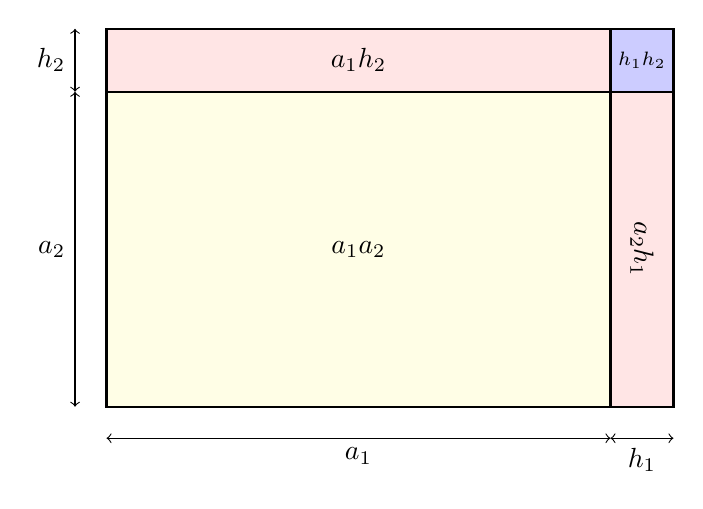
\begin{tikzpicture}[scale=0.8]
    % 原始长方形
    \fill[yellow!10] (0,0) rectangle (8,5);
    \draw[thick] (0,0) rectangle (8,5);
    \node at (4, 2.5) {$a_1 a_2$};
    
    % 延伸的水平部分
    \fill[red!10] (8,0) rectangle (9,5);
    \draw[thick] (8,0) rectangle (9,5);
    \node[rotate=270] at (8.5,2.5) {$a_2  h_1$};
    
    % 延伸的垂直部分
    \fill[red!10] (0,5) rectangle (8,6);
    \draw[thick] (0,5) rectangle (8,6);
    \node at (4,5.5) {$a_1 h_2$};
    
    % 拐角的小矩形
    \fill[blue!20] (8,5) rectangle (9,6);
    \draw[thick] (8,5) rectangle (9,6);
    \node at (8.5,5.5) {$\scriptstyle h_1 h_2$};
    
    % 标注尺寸
    \draw[<->] (-0.5,0) -- (-0.5,5) node[midway,left] {$a_2$};
    \draw[<->] (0,-0.5) -- (8,-0.5) node[midway,below] {$a_1$};
    
    % \draw[<->] (9.5,0) -- (9.5,5) node[midway,right] {$a_2$};
    \draw[<->] (8,-0.5) -- (9,-0.5) node[midway,below] {$h_1$};
    
    % \draw[<->] (0,4.4) -- (4,4.4) node[midway,above] {$a_1$};
    \draw[<->] (-0.5,5) -- (-0.5,6) node[midway,left] {$h_2$};
    
    % 箭头指向总面积
    % \draw[->, thick] (6,4.5) -- (5,3.5);
    % \node[right] at (6,4.5) {总面积：$(a_1+h_1)(a_2+h_2)$};
    
    % 颜色说明
    % \node[blue] at (7,2) {蓝色：$a_2 \cdot h_1$（长增加带来的面积）};
    % \node[red] at (7,1.5) {红色：$a_1 \cdot h_2$（宽增加带来的面积）};
    % \node[green] at (7,1) {绿色：$h_1 \cdot h_2$（二阶小量，可忽略）};
\end{tikzpicture}
% \caption*{长方形面积变化的分解示意图}
\end{figure}


\begin{et}
    计算函数$f(x,y) = \sin(xy)$的微直观，以及在$\left(0, \frac{\pi}{2}\right)$处的全微变。
\end{et}

\begin{so}
    首先计算偏微变：
    $$ \partial_1 f(x,y) = y\cos(xy), \quad \partial_2 f(x,y) = x\cos(xy). $$
    因此，微直观为：
    $$ (h_1, h_2) \mapsto \partial_1 f(x,y)h_1 + \partial_2 f(x,y)h_2 = y\cos(xy)h_1 + x\cos(xy)h_2. $$
    在$\left(0, \frac{\pi}{2}\right)$处，$(h_1, h_2)$带来的变化为：
    \begin{align*}
        \Delta f(\mathbf{a}) &\approx \frac{\pi}{2}\cdot\cos{\left(0\cdot \frac{\pi}{2}\right)}h_1 + 0\cdot\cos{\left(0\cdot \frac{\pi}{2}\right)}h_2 \\
        &= \frac{\pi}{2} h_1
    \end{align*}
    也就是说，曲面在$\left(0, \frac{\pi}{2}\right)$处，沿$x$轴增长$h_1$为函数值带来的变化约为$\frac{\pi}{2} h_1$，沿$y$轴增长$h_2$带来的变化则是$h_2$的高阶无穷小。
\end{so}

对于多个可微函数，我们可以通过它们各自的全微变，计算它们四则运算后的全微变。例如，对于两个在$\mathbf{a}$处可微的二元函数$f$和$g$，以及常数$c$，我们有：
\begin{align*}
    \Delta (f\pm g)(\mathbf{a}) &= \Delta f(\mathbf{a}) \pm \Delta g(\mathbf{a}), \\
    \Delta (fg)(\mathbf{a}) &= f(\mathbf{a})\cdot \Delta g(\mathbf{a}) + g(\mathbf{a})\cdot \Delta f(\mathbf{a}), \\
    \Delta(cf)(\mathbf{a}) &= c\cdot \Delta f(\mathbf{a}), \\
    \Delta\left(\frac{f}{g}\right)(\mathbf{a}) &= \frac{g(\mathbf{a})\cdot \Delta f(\mathbf{a}) - f(\mathbf{a})\cdot \Delta g(\mathbf{a})}{g^2(\mathbf{a})} \quad \left(\mbox{当}g(\mathbf{a})\neq 0\mbox{时}\right).
\end{align*}
这些性质的证明与方向微变的运算法则类似。

\begin{sk}
\mbox{}\\
\indent 1. 如果二元函数在一点的偏微变存在，但不可微，这时，依照偏微变构建的维直变换对应的平面和原曲面会有什么可能的关系？举一些典型的例子来说明你的想法。\\
\indent 2. 如果$Oxy$平面上发生了基底变换，原基底$\mathbf{e}_x, \mathbf{e}_y, \mathbf{e}_z$变成了$\mathbf{e}_x', \mathbf{e}_y', \mathbf{e}_z$，这种变换如何影响可微二元函数的切平面的方程？切平面是否改变？
\end{sk}

\begin{xt}
    \mbox{}\\
    \indent 1. 证明以下函数在指定点$\mathbf{a}$处可微，并计算其全微变：
    \begin{align*}
    1).& \quad f(x,y) = x^3 + y^3 - 3xy, \quad \mathbf{a} = (1,1) \\
    2).& \quad g(x,y) = e^{x+y}\cos(x-y), \quad \mathbf{a} = (0,0) \\
    3).& \quad h(x,y) = \ln(x^2+y^2+1), \quad \mathbf{a} = (1,0)
    \end{align*}
    \indent 2. 证明以下函数在$(0,0)$处偏微变存在，但不可微：
    $$ f(x,y) = \begin{cases}
    \dfrac{xy}{\sqrt{x^2+y^2}} & \text{若 } (x,y)\neq(0,0), \\
    0 & \text{若 } (x,y)=(0,0).
    \end{cases} $$
    \indent 3. 设$f(x,y) = x^2y + 2xy^2$，利用全微变计算$f(1.01,1.98)$的近似值。\\
    \indent 4. 证明本节最后，函数的四则运算对应的全微变公式。
\end{xt}

\section{曲面上一点的梯度}
我们已经看到，如果二元函数$f$在点$\mathbf{a}$处可微，那么有平直变换$\diff f(\mathbf{a})$，使得当$\mathbf{h}$很小时，
$$ f(\mathbf{a} + \mathbf{h}) - f(\mathbf{a}) = \diff f(\mathbf{a})(\mathbf{h}) + \olim{|\mathbf{h}|}, $$
其中$\diff f(\mathbf{a})$由$f$在$\mathbf{a}$处的偏微变唯一确定：
$$ \diff f(\mathbf{a})(\mathbf{h}) = h_1 \partial_1 f(\mathbf{a}) + h_2 \partial_2 f(\mathbf{a}). $$
多元函数的微变是平直变换，是不是就没办法用一个量来代表它了呢？也不尽然。考虑平面经典内积的话，可以把$\diff f(\mathbf{a})$表示为：
$$ \forall\; \mathbf{h} = (h_1, h_2)\in \mathbb{R}^2, \quad \diff f(\mathbf{a})(\mathbf{h}) = \nji{\mathbf{h}}{\nabla_f(\mathbf{a})}, $$
其中$\nabla_f(\mathbf{a}) = (\partial_1 f(\mathbf{a}), \partial_2 f(\mathbf{a}))$。我们把这个向量$\nabla_f(\mathbf{a})$叫做函数$f$在点$\mathbf{a}$处的\textbf{梯度}。

梯度有什么直观意义呢？考虑从点$\mathbf{a}$出发，沿单位向量$\mathbf{v}$方向移动微小距离$t$。函数值的变化为：
$$ f(\mathbf{a} + t \mathbf{v}) - f(\mathbf{a}) = t \diff f(\mathbf{a})(\mathbf{v}) + \olim{t} = t \cdot \nji{\mathbf{v}}{\nabla_f(\mathbf{a})}  + \olim{t}. $$
根据内积不等式，
$$ -|\mathbf{v}|\cdot |\nabla_f(\mathbf{a})| \leqslant \nji{\mathbf{v}}{\nabla_f(\mathbf{a})} \leqslant |\mathbf{v}|\cdot |\nabla_f(\mathbf{a})|. $$
由于$\mathbf{v}$是单位向量，$|\mathbf{v}| = 1$，因此当$\mathbf{v}$与$\nabla_f(\mathbf{a})$同向时，$\nji{\mathbf{v}}{\nabla_f(\mathbf{a})}$达到最大值$|\nabla_f(\mathbf{a})|$；当$\mathbf{v}$与$\nabla_f(\mathbf{a})$反向时，达到最小值$-|\nabla_f(\mathbf{a})|$。

梯度向量与方向微变有密切关系。$f$沿单位向量$\mathbf{v}$方向的微变为：
\begin{align*}
\partial_{\mathbf{v}} f(\mathbf{a}) &= \nji{\mathbf{v}}{\nabla_f(\mathbf{a})} \\
&= |\mathbf{v}|\cdot |\nabla_f(\mathbf{a})| \cdot \cos\theta \\
&= |\nabla_f(\mathbf{a})| \cdot \cos\theta,
\end{align*}
其中$\theta$是$\mathbf{v}$与$\nabla_f(\mathbf{a})$的夹角。这说明方向微变是梯度大小乘以夹角的余弦。方向微变表示沿此方向变动时，函数值的变化。因此，函数值的变化在梯度方向最快，而在垂直梯度方向最不明显。

为了帮助理解，可以把函数值变化量写成这样：
$$ f(\mathbf{a} + t \mathbf{v}) - f(\mathbf{a}) = t \cdot |\mathbf{v}| \cdot |\nabla_f(\mathbf{a})| \cdot \frac{\nji{\mathbf{v}}{\nabla_f(\mathbf{a})}}{|\mathbf{h}|\cdot|\nabla_f(\mathbf{a})|}  + \olim{t} =  t \cdot |\nabla_f(\mathbf{a})| \cdot \cos{\theta}  + \olim{t}.$$
其中$\theta$是向量$\mathbf{v}$和梯度向量$\nabla_f(\mathbf{a})$的夹角。直观来说，$t$很小的时候，往任意方向移动$t$长度，函数值的变化量就和移动向量在梯度向量上的投影长度成正比。投影长度小于等于移动向量的原长度。如果移动的方向与梯度向量相同或相反，那么投影长度就是原长度，于是函数值变化得最快。可以理解为，在梯度方向上的微小移动，对函数值变化的“效率”是最高的。从点$\mathbf{a}$出发，沿着梯度方向$\nabla_f(\mathbf{a})$移动，函数值增长最快；沿着梯度的反方向移动，函数值下降最快。梯度的大小$|\nabla_f(\mathbf{a})|$表示函数在该点的最大增长率，梯度的方向是函数值局部增长最快的方向。

\begin{et}
计算函数$f(x,y) = x^2 + y^2$在点$P=(1,2)$处的梯度，解释其直观意义。
\end{et}
\begin{so}
首先计算偏微变：
$$ \partial_1 f(x,y) = 2x, \quad \partial_2 f(x,y) = 2y. $$
在点$(1,2)$处：
$$ \nabla_f(1,2) = (\partial_1 f(1,2), \partial_2 f(1,2)) = (2, 4). $$
这说明在$(1,2)$处，函数$f$的增长最快方向是向量$(2,4)$的方向。而函数值在该方向的增长率为$\sqrt{2^2 + 4^2} = 2\sqrt{5}$。直观上看，函数的曲面是一个旋转抛物面，方程为$z = x^2 + y^2$。$f(1,2) = 5$，对应曲面上点$Q=(1,2,5)$，切平面方程为
$$\gamma_{(1,2)}: \;z = 2(x - 1) + 4(y - 2) + 5 = 2x + 4y - 5. $$
梯度向量$(2,4)$是一个平面向量，它说明自变量（$Oxy$平面上的点）$(x,y)$沿着$(2,4)$方向移动时，$f$的值变化最快。我们可以作过$(x,y)$垂直于$Oxy$的竖直直线，研究它自$(1,2)$略微移动时，直线和曲面、切平面的交点的变化，来查看两者的增长方式。具体来说，比如从$(1,2)$移动到$(1.1,2.2)$时，直线和曲面的交点高度从$5$变为$6.05$，而直线和切平面的交点高度从$5$变为$6$。所以在切平面，梯度方向的向量为$(1,2,10)$。而如果我们的移动垂直于$(2,4)$，比方说从$(1,2)$移动到$(1.2, 1.9)$（移动量为$(0.2, -0.1)$），则直线与切平面交点高度还是$5$，没有变化（直线和曲面交点高度变为$5.05$）。我们可以把切平面写作经过$\mathbf{u}=(1,2,5)$，以$\mathbf{e}_1 = (1,2,10)$和$\mathbf{e}_2 = (2,-1,0)$为基底构成的平面：
$$ \gamma_{(1,2)} = \left\{ \mathbf{u} + s\mathbf{e}_1 + t\mathbf{e}_2 \; | \; s, t \in \mathbf{R}\right\} $$
沿$\mathbf{e}_2$方向，函数$f$变化最快，沿$\mathbf{e}_2$方向，$f$变化最不明显（实际上是等高线的切线）。
\end{so}

\begin{figure}[h]
\centering
\begin{tikzpicture}
    \begin{axis}[
        width=12cm,
        height=10cm,
        view={120}{30},
        axis lines=middle,
        xlabel=$x$,
        ylabel=$y$,
        zlabel=$z$,
        zmin=0,
        zmax=10,
        xmin=-2,
        xmax=4,
        ymin=-2.3,
        ymax=6,
        grid=major,
        xtick distance=1,
        ytick distance=1,
        % colormap/viridis,
        ticklabel style={font=\small},
        label style={font=\small},
        samples=30,
        domain=-2.3:4,
        y domain=-2.3:6,
        z buffer=sort
    ]
    
    % --- 定义函数 f(x,y) = x^2 + y^2 ---
    \pgfmathdeclarefunction{QuadraticFunc}{2}{\pgfmathparse{(#1)^2 + (#2)^2}}
    
    % --- 绘制等高线 ---
    % 在z=5处，x^2+y^2=5，所以半径为sqrt(5)
    \draw[blue, thick, dashed] 
        plot[domain=110:310, samples=100] 
        ({sqrt(5)*cos(\x)}, {sqrt(5)*sin(\x)}, {5});
    % --- 绘制等高线 ---
    % 在z=5处，x^2+y^2=5，所以半径为sqrt(5)
    \draw[Sepia, thick, opacity=0.5] 
        plot[domain=0:360, samples=100] 
        ({sqrt(5)*cos(\x)}, {sqrt(5)*sin(\x)}, {0});

    % --- 绘制曲面 z = x^2 + y^2 ---
    \addplot3[
        surf,
        % shader=faceted interp,
        colormap/autumn,
        opacity=0.7,
        domain=-2.3:2.5, 
        y domain=-2.3:2.5
    ] {QuadraticFunc(x, y)};

    % --- 绘制等高线 ---
    % 在z=5处，x^2+y^2=5，所以半径为sqrt(5)
    \draw[Sepia, thick] 
        plot[domain=-50:110, samples=100] 
        ({sqrt(5)*cos(\x)}, {sqrt(5)*sin(\x)}, {5});
    
    % --- 绘制切平面 z = 2x + 4y - 5 (在点(1,2,5)处) ---
    % 切平面：z = 2x + 4y - 5，切点 (1,2,5)
    % 网格线数量固定为5（确保切点在网格交点上）
    % 水平方向：与梯度垂直的方向（等z线方向）
    % 竖直方向：梯度在xy平面的投影方向 (2,4)

    % ==================== 关键参数设置 ====================
    % 矩形在水平方向的半宽（调整此值改变矩形宽度）
    \def\recWidth{2.0}
    % 矩形在竖直方向的半高（调整此值改变矩形高度）
    \def\recHeight{1.6}

    % ==================== 方向向量计算 ====================
    % 水平方向：与梯度(2,4)垂直的向量，取(-4,2)，然后单位化
    \pgfmathsetmacro{\horizLength}{sqrt((-4)^2 + 2^2)}
    \pgfmathsetmacro{\unitHorizX}{-4/\horizLength}  % 水平单位向量x分量
    \pgfmathsetmacro{\unitHorizY}{2/\horizLength}   % 水平单位向量y分量

    % 竖直方向：梯度在xy平面的投影(2,4)，单位化
    \pgfmathsetmacro{\vertLength}{sqrt(2^2 + 4^2)}
    \pgfmathsetmacro{\unitVertX}{2/\vertLength}     % 竖直单位向量x分量
    \pgfmathsetmacro{\unitVertY}{4/\vertLength}     % 竖直单位向量y分量

    % ==================== 绘制切平面 ====================
    \addplot3[
        surf,
        shader=flat,
        colormap/cool,
        opacity=0.5,
        domain=-0.5:0.5,      % 参数u：水平方向参数，范围[-0.5, 0.5]
        y domain=-0.5:0.5,    % 参数v：竖直方向参数，范围[-0.5, 0.5]
        samples=5,            % 水平方向网格线数（固定为5）
        samples y=5,          % 竖直方向网格线数（固定为5）
    ] 
    ({1 + \recWidth*x*\unitHorizX + \recHeight*y*\unitVertX},
    {2 + \recWidth*x*\unitHorizY + \recHeight*y*\unitVertY},
    {2*(1 + \recWidth*x*\unitHorizX + \recHeight*y*\unitVertX) + 
    4*(2 + \recWidth*x*\unitHorizY + \recHeight*y*\unitVertY) - 5});
    
    % --- 绘制切向量在xy平面上 ---
    \draw[Sepia!75, dashed] (axis cs:3,1,0) -- (axis cs:-1,3,0);
    % --- 绘制直角在xy平面上 ---
    \draw[Sepia] (axis cs:0.8,2.1,0) -- (axis cs:0.9,2.3,0);
    \draw[Sepia] (axis cs:1.1,2.2,0) -- (axis cs:0.9,2.3,0);
    % --- 绘制梯度向量 (2,4) 在xy平面上 ---
    \draw[-Stealth, red, thick] (axis cs:1,2,0) -- (axis cs:3,6,0);
    % --- 绘制梯度向量对应的切平面增长向量 ---
    \draw[-Stealth, Plum, thick] (axis cs:1,2,5) -- (axis cs:1.15,2.3,6.5);
    % --- 绘制梯度向量对应的切平面水平向量 ---
    \draw[-Stealth, Plum!80, thick] (axis cs:1,2,5) -- (axis cs:0.5,2.25,5);
    
    % --- 标记点 (1,2,5) ---
    \fill[black] (axis cs:1,2,5) circle (2pt) node[above left] {$Q$};
    \fill[black] (axis cs:1,2,0) circle (2pt) node[below] {$P$};
    
    % --- 绘制从点(1,2)到(1,2,5)的垂线 ---
    \draw[dashed] (axis cs:1,2,0) -- (axis cs:1,2,5);
    \draw[dashed,opacity=0.5] (axis cs:1,0,0) -- (axis cs:1,2,0);
    \draw[dashed,opacity=0.5] (axis cs:0,2,0) -- (axis cs:1,2,0);
        
    % --- 添加标签 ---
    \node[black] at (axis cs:1,-1.7,9) {$z=x^2+y^2$};
    \node[blue] at (axis cs:1,4,5) {\texttt{切平面}};
    \node[Sepia] at (axis cs:2,-2,0) {\texttt{等高线}};
    \node[red] at (axis cs:3.1,3.2,0) {$\nabla_f(1,2) = (2,4)$};
    
    \end{axis}
\end{tikzpicture}
% \caption{函数 $f(x,y) = x^2 + y^2$ 在点 $(1,2)$ 处的梯度示意图。红色向量表示梯度方向，是函数值增长最快的方向。梯度向量垂直于等高线，指向函数值增加的方向。}
\end{figure}

\begin{tm}{\textbf{梯度的运算性质}}
设$\mathbb{R}^2$上的函数$f, g$在$\mathbf{a}$处可微，则：
\begin{enumerate}[label=\arabic*.]
\item $\nabla_{f \pm g}(\mathbf{a}) = \nabla_f(\mathbf{a}) \pm \nabla_g(\mathbf{a})$
\item 设$c$为常数，则$\nabla_{cf}(\mathbf{a}) = c\cdot \nabla_f(\mathbf{a})$
\item $\nabla_{f\cdot g}(\mathbf{a}) = g(\mathbf{a})\cdot \nabla_f(\mathbf{a}) + f(\mathbf{a})\cdot \nabla_g(\mathbf{a})$
\item 若$g(\mathbf{a}) \neq 0$，则$\displaystyle\nabla_{\frac{f}{g}}(\mathbf{a}) = \frac{g(\mathbf{a})\cdot \nabla_f(\mathbf{a}) - f(\mathbf{a})\cdot \nabla_g(\mathbf{a})}{g^2(\mathbf{a})}$
\end{enumerate}
\end{tm}
\begin{proof}
这些性质可以从偏微变的运算性质直接推导。以乘积法则为例：
\begin{align*}
\nabla(fg)(\mathbf{a}) &= (\partial_1(fg)(\mathbf{a}), \partial_2(fg)(\mathbf{a})) \\
&= (g(\mathbf{a})\cdot \partial_1 f(\mathbf{a}) + f(\mathbf{a})\cdot \partial_1 g(\mathbf{a}),\,\, g(\mathbf{a})\cdot \partial_2 f(\mathbf{a}) + f(\mathbf{a})\cdot \partial_2 g(\mathbf{a})) \\
&= g(\mathbf{a})\cdot (\partial_1 f(\mathbf{a}), \partial_2 f(\mathbf{a})) + f(\mathbf{a})\cdot (\partial_1 g(\mathbf{a}), \partial_2 g(\mathbf{a})) \\
&= g(\mathbf{a})\cdot \nabla_f(\mathbf{a}) + f(\mathbf{a})\cdot \nabla_g(\mathbf{a}).
\end{align*}
其他性质可类似证明。
\end{proof}

\begin{et}
考虑两条与$z$轴平行的无限长直导线，分别通过点$(-d,0)$和$(d,0)$，其中$d=0.1\,\mathrm{m}$。第一条导线带正电，线电荷密度为$+a$；第二条导线带负电，线电荷密度为$-a$。

在$Oxy$平面中，这两条导线产生的电势分布为：
$$ V(x,y) = \frac{a}{4\pi\epsilon_0} \ln\left(\frac{(x-d)^2+y^2}{(x+d)^2+y^2}\right) $$
其中$\epsilon_0 = 8.854\times10^{-12}\,\mathrm{F/m}$是真空介电常数。

\indent 1. 计算电势函数$V$在点$P(0,d)$处的梯度$\nabla_V(0,d)$。\\
\indent 2. 设导线的线电荷密度为$a=3\times10^{-5}\,\mathrm{C/m}$，若将一个电荷量为$q=2\times10^{-6}\,\mathrm{C}$的带电小球置于点$P$，计算它受到的电场力。
\end{et}

\begin{figure}[h]
\centering 
\begin{tikzpicture}[scale=0.72]  
    \begin{scope}[shift={(0,0)}]
    \def\d{2} % 导线半间距 d
    \def\xmax{7.5}
    \def\ymax{4}

    % 坐标轴
    \draw[-Stealth, thick] (-\xmax-0.5, 0) -- (\xmax+0.5, 0) node[right] {$x$};
    \draw[-Stealth, thick] (0, -\ymax-0.5) -- (0, \ymax+0.5) node[above] {$y$};
    \node at (-0.3,-0.3) {$O$};

    % ========== 绘制等势线 (Equipotential Circles) ==========
    % 使用阿波罗尼斯圆公式：k 取不同值
    \foreach \k in {0.05,0.1,0.1667, 0.25, 0.333,0.4167,2.4,3, 4, 6, 10, 20} {
        \pgfmathsetmacro{\xc}{\d * (1 + \k) / (1 - \k)}
        \pgfmathsetmacro{\radius}{\d * 2 * sqrt(\k) / abs(1 - \k)}
        \draw[orange!80!black, thin, opacity=0.6] (\xc, 0) circle (\radius);
    }
    \draw[orange!80!black, thin, opacity=0.6, domain=-52.70:52.70, samples=200] plot ({-6.00+5.66*cos(\x)},{5.66*sin(\x)});
    \draw[orange!80!black, thin, opacity=0.6, domain=-52.70:52.70, samples=200] plot ({6.00-5.66*cos(\x)},{5.66*sin(\x)});
    \draw[orange!80!black, thin, opacity=0.6, domain=-35.52:35.52, samples=200] plot ({-8.00+7.75*cos(\x)},{7.75*sin(\x)});
    \draw[orange!80!black, thin, opacity=0.6, domain=-35.52:35.52, samples=200] plot ({8.00-7.75*cos(\x)},{7.75*sin(\x)});
    \draw[orange!80!black, thin, opacity=0.6, domain=-14.57:14.57, samples=200] plot ({-18.00+17.89*cos(\x)},{17.89*sin(\x)});
    \draw[orange!80!black, thin, opacity=0.6, domain=-14.57:14.57, samples=200] plot ({18.00-17.89*cos(\x)},{17.89*sin(\x)});

    % ========== 绘制电场线 (Electric Field Arcs) ==========
    % 电场线是经过 (-d,0) 和 (d,0) 的圆弧
    \foreach \yc in {-1.5, -1, -0.5, 0, 0.5, 1, 1.5} {
        \pgfmathsetmacro{\radius}{sqrt(\d*\d + \yc*\yc)}
        \draw[CadetBlue] (0, {\yc}) circle (\radius);
    }
    \draw[CadetBlue] (-\d,0) arc [start angle=225.00, delta angle=197.11, radius=2.828];
    \draw[CadetBlue] (-\d,0) arc [start angle=225.00, delta angle=-107.11, radius=2.828];
    \draw[CadetBlue] (-\d,0) arc [start angle=135.00, delta angle=-197.11, radius=2.828];
    \draw[CadetBlue] (-\d,0) arc [start angle=135.00, delta angle=107.11, radius=2.828];
    \draw[CadetBlue] (-\d,0) arc [start angle=236.31, delta angle=148.27, radius=3.606];
    \draw[CadetBlue] (-\d,0) arc [start angle=236.31, delta angle=-80.89, radius=3.606];
    \draw[CadetBlue] (-\d,0) arc [start angle=123.69, delta angle=-148.27, radius=3.606];
    \draw[CadetBlue] (-\d,0) arc [start angle=123.69, delta angle=80.89, radius=3.606];
    \draw[CadetBlue] (-\d,0) arc [start angle=243.43, delta angle=122.98, radius=4.472];
    \draw[CadetBlue] (-\d,0) arc [start angle=243.43, delta angle=-69.85, radius=4.472];
    \draw[CadetBlue] (-\d,0) arc [start angle=116.57, delta angle=-122.98, radius=4.472];
    \draw[CadetBlue] (-\d,0) arc [start angle=116.57, delta angle=69.85, radius=4.472];
    \draw[CadetBlue] (-\d,0) arc [start angle=251.56, delta angle=94.72, radius=6.325];
    \draw[CadetBlue] (-\d,0) arc [start angle=251.56, delta angle=-57.85, radius=6.325];
    \draw[CadetBlue] (-\d,0) arc [start angle=108.44, delta angle=-94.72, radius=6.325];
    \draw[CadetBlue] (-\d,0) arc [start angle=108.44, delta angle=57.85, radius=6.325];
    \draw[CadetBlue] (-\d,0) arc [start angle=258.69, delta angle=62.98, radius=10.198];
    \draw[CadetBlue] (-\d,0) arc [start angle=258.69, delta angle=-40.36, radius=10.198];
    \draw[CadetBlue] (-\d,0) arc [start angle=101.31, delta angle=-62.98, radius=10.198];
    \draw[CadetBlue] (-\d,0) arc [start angle=101.31, delta angle=40.36, radius=10.198];
    \draw[CadetBlue] (-\d,0) arc [start angle=264.29, delta angle=29.17, radius=20.100];
    \draw[CadetBlue] (-\d,0) arc [start angle=264.29, delta angle=-17.74, radius=20.100];
    \draw[CadetBlue] (-\d,0) arc [start angle=95.71, delta angle=-29.17, radius=20.100];
    \draw[CadetBlue] (-\d,0) arc [start angle=95.71, delta angle=17.74, radius=20.100];
    % ========== 标注电荷位置 ==========
    \fill[red] (-\d, 0) circle (3pt); % node[below left, black] {$+a$};
    \draw[white,thick] (-\d-0.1,0) -- (-\d+0.1,0) (-\d,-0.1) -- (-\d,+0.1);
    \fill[blue] (\d, 0) circle (3pt); % node[below right, black] {$-a$};
    \draw[white,thick] (\d-0.1,0) -- (\d+0.1,0);

    % ========== 梯度与电场力分析 (以点 (0, d) 为例) ==========
    \coordinate (P) at (0, \d);
    % 梯度向量 \nabla_V (指向电势增加的方向，即指向正电荷)
    \draw[-Stealth, very thick, ForestGreen] (P) -- (-1.2, \d); 
    % 电场力 F (假设带正电荷 q)
    \draw[-Stealth, very thick, Purple] (P) -- (2.0, \d) ;
    \fill[black] (P) circle (2pt); 
    \node at (-0.3,\d+0.3) {$P$};

    \def\lx{6};
    \def\xpd{0.2};
    \def\lbar{0.3};
    \def\rc{0.9};
    \def\lb{1};
    \def\g{0.8};
    \def\pad{0.5}
    \draw[thick,fill=white] (\lx,\lb) rectangle (\lx+3*\xpd+\lbar+2*\rc,\lb+2*\pad+3*\g);
    \draw[thick, Purple] (\lx+\xpd,\lb+\pad) -- (\lx+\xpd+\lbar,\lb+\pad);
    \draw[thick, ForestGreen] (\lx+\xpd, \lb+\pad+1*\g) -- (\lx+\xpd+\lbar,\lb+\pad+1*\g);
    \draw[thick, CadetBlue] (\lx+\xpd, \lb+\pad+2*\g) -- (\lx+\xpd+\lbar,\lb+\pad+2*\g);
    \draw[thick, orange!80!black] (\lx+\xpd,\lb+\pad+3*\g) -- (\lx+\xpd+\lbar,\lb+\pad+3*\g);
    \node at (\lx+\xpd+\lbar+\rc,\lb+\pad) {$\mbox{\footnotesize \texttt{电场力}}$};
    \node at (\lx+\xpd+\lbar+\rc+0.2,\lb+\pad+1*\g) {$\mbox{\footnotesize \texttt{电势梯度}}$};
    \node at (\lx+\xpd+\lbar+\rc,\lb+\pad+2*\g) {$\mbox{\footnotesize \texttt{电场线}}$};
    \node at (\lx+\xpd+\lbar+\rc,\lb+\pad+3*\g) {$\mbox{\footnotesize \texttt{等势线}}$};
    
    \end{scope}
\end{tikzpicture}
\caption*{\texttt{平行带电导线系统电势图}}
\end{figure}

\begin{so}
首先计算电势函数$V(x,y)$关于$x$的偏微变（将$y$视为常数）：
\begin{align*}
\partial_1 V(x,y) &= \frac{a}{4\pi\epsilon_0} \left( \partial_x \ln{\left( (x-d)^2+y^2\right)} - \partial_x \ln{\left( (x+d)^2+y^2\right)} \right) \\
&= \frac{a}{4\pi\epsilon_0} \left( \frac{2(x-d)}{(x-d)^2+y^2} - \frac{2(x+d)}{(x+d)^2+y^2} \right) \\
&= \frac{a}{2\pi\epsilon_0} \left( \frac{x-d}{(x-d)^2+y^2} - \frac{x+d}{(x+d)^2+y^2} \right)
\end{align*}

类似地，计算$V$关于$y$的偏微变（将$x$视为常数）：
\begin{align*}
\partial_2 V(x,y) &= \frac{a}{4\pi\epsilon_0} \left( \partial_y \ln{\left( (x-d)^2+y^2\right)} - \partial_y \ln{\left( (x+d)^2+y^2\right)} \right) \\
&= \frac{a}{4\pi\epsilon_0} \left( \frac{2y}{(x-d)^2+y^2} - \frac{2y}{(x+d)^2+y^2} \right) \\
&= \frac{a y}{2\pi\epsilon_0} \left( \frac{1}{(x-d)^2+y^2} - \frac{1}{(x+d)^2+y^2} \right)
\end{align*}

电势函数在$(x,y)$处的梯度为：
$$ \nabla_V(x,y) = \left(\partial_1 V(x,y), \partial_2 V(x, y)\right).$$
将$x=0$，$y=d$代入表达式中，得到：
\begin{align*}
\partial_1 V(0,d) &= \frac{a}{2\pi\epsilon_0} \left( \frac{-d}{d^2+d^2} - \frac{d}{d^2+d^2} \right) = -\frac{a}{2\pi\epsilon_0 d} \\
\partial_2 V(0,d) &=\frac{a y}{2\pi\epsilon_0} \left( \frac{1}{d^2+d^2} - \frac{1}{d^2+d^2} \right) = 0
\end{align*}
因此，电势函数在$P$处的梯度为：
$$ \nabla_V(0,d) = \left( -\frac{a}{2\pi\epsilon_0 d}, 0 \right).$$
它指向$x$轴负方向。

在静电学中，电场力$\mathbf{F}$与电势梯度满足以下关系：
$$ \mathbf{F} = q\mathbf{E} = -q\nabla_V $$
其中$\mathbf{E}$是电场强度。代入数值，得到：
\begin{align*}
\mathbf{F} &= -q\nabla_V(0,d) = \left( \frac{qa}{2\pi\epsilon_0 d}, 0 \right) =\left( \frac{2\times10^{-6}\,\mathrm{C} \times 3\times10^{-5}\mathrm{C/m} }{2\pi\times 8.854\times10^{-12}\,\mathrm{F/m}\times 0.1\mathrm{m}}, 0 \right)\\
&= 10.79\,\mathrm{N}
\end{align*}
答：带电小球在电场中受到$10.79\,\mathrm{N}$的电场力，方向为$x$轴正方向。
\end{so}

% \begin{et}
% 设关于$x,y$的二元函数$z$由方程$x^2 + y^2 + z^2 = 1$隐式定义，计算梯度$\nabla_z(x,y)$。
% \end{et}
% \begin{so}
% 将$z$与$x,y$的关系记为$f: (x,y)\mapsto z$。我们不知道其表达式，只知道它满足方程$x^2 + y^2 + z^2 = 1$。考虑三元函数$F:\, (x,y,z) \mapsto x^2 + y^2 + z^2 - 1$。则$\forall x,y\in[-1;1]$，$F(x,y,f(x,y)) = 0$。这说明映射：$H: \,(x,y)\mapsto F(x,y,f(x,y))$是常函数。对映射$H$求偏微变：
% \begin{align*}
% 0 &= \partial_1 H(x,y) = \partial_1 F(x,y,f(x,y)) + \partial_3 F(x,y,f(x,y)) \cdot \partial_1 f(x,y) \\
% 0 &= \partial_2 H(x,y) = \partial_2 F(x,y,f(x,y)) + \partial_3 F(x,y,f(x,y)) \cdot \partial_2 f(x,y)
% \end{align*}
% 由$F$的表达式，可算出$\partial_1 F(x,y,z) = 2x$, $\partial_2 F(x,y,z) = 2y$, $\partial_3 F(x,y,z) = 2z$。于是$z = f(x,y)\neq 0$时，可得：
% \begin{align*}
%     2x + 2f(x,y) \cdot \partial_1 f(x,y) &= 0 \quad \Rightarrow \quad \partial_1 z = -\frac{x}{z} \\
%     2y + 2f(x,y) \cdot \partial_2 f(x,y) &= 0 \quad \Rightarrow \quad \partial_2 z = -\frac{y}{z}
% \end{align*}
% 因此，
% $$ \nabla_z(x,y) = \left(-\frac{x}{z}, -\frac{y}{z}\right) = -\frac{1}{z}(x,y). $$
% 从直观上看，这个结果表示$z\neq 0$时，球面$x^2 + y^2 + z^2 = 1$在平面上一点$(x,y)$处的高度$z$的梯度方向是该点在$Oxy$平面上的投影到原点的方向。换句话说，$z>0$时，点$(x,y,z)$向球的北极点走，$z$增长最快；$z<0$时，点$(x,y,z)$向球的南极点走，$z$降低最快。这与球面的直观性质一致。
% \end{so}

需要注意的是，梯度向量的存在依赖于函数在该点的可微性。我们已知函数在某点的偏微变存在，并不代表函数在该点可微。如果函数在点$\mathbf{a}$处不可微，那么即使能构造出形式上的梯度向量，它也不能正确描述函数在该点附近的变化。例如，考虑函数：
$$ f(x,y) = \begin{cases}
\dfrac{xy}{\sqrt{x^2+y^2}} & \text{若 } (x,y) \neq (0,0), \\
0 & \text{若 } (x,y) = (0,0).
\end{cases} $$
虽然$f$在$(0,0)$处的偏微变存在且均为$0$，但$f$在该点不可微。此时，形式上的梯度向量$\nabla_f(0,0) = (0,0)$不能描述函数在原点附近的真实变化。比如，考虑$(1,k)$方向上函数的变化。令$x = t, y = kt$。代入表达式得到
$$ f(x, y) = \frac{t\cdot kt}{\sqrt{t^2 + k^2t^2}} = \frac{k}{\sqrt{k^2 + 1}}\cdot t.$$
$t$增大时，$f$的值成比例增加。偏微分构成的$(0,0)$向量无法描述$f$在$(0,0)$附近的变化了。
因此，在使用梯度之前，必须先验证函数在该点的可微性。

学习实函数时，我们证明了中值定理。中值定理为我们搭建了函数局部性质与整体行为之间的桥梁。那么，多元函数是否有类似的结论呢？回顾实函数的中值定理，我们看到，中值定理描述函数在线段$[a,b]$上的性质，而二元函数的定义域则是平面的点集。对于二元函数来说，连接定义域内$\mathbf{a}, \mathbf{b}$两点，函数值从$\mathbf{a}$到$\mathbf{b}$的变化趋势，是否也能用两点连线上的一点的微变性质表示呢？

作为讨论的前提，我们希望函数在两点的连线上总有定义。为了方便说话，我们引入凸集的概念：
\begin{df}{\textbf{凸集}}
如果集合$D\subseteq \mathbb{R}^2$中任意两点$\mathbf{a},\mathbf{b}$的连线段全部位于$D$内，即对任意$t\in[0,1]$，点$t\mathbf{a}+(1-t)\mathbf{b}$都属于$D$，就说$D$是\textbf{凸集}。
\end{df}

凸集的直观意义是：集合中任意两点之间的连线完全包含在集合内。常见的凸集包括圆盘、矩形区域等。假设定义域为凸集，或者在定义域中划出一个凸集作为邻域，我们就可以讨论其中两点的连线，以及中值定理了。中值定理的整体想法是：函数在两点间的变化量，等于函数在两点连线上某点的梯度与位移向量的内积，换句话说，我们总能找到某点的梯度来代表整体的趋势。这与一元函数中值定理的思想一脉相承，只是将标量乘法扩展为向量内积。

\begin{tm}
设二元函数$f$在凸集$D\subseteq \mathbb{R}^2$上可微，$\mathbf{a},\mathbf{b}\in D$。则存在点$\mathbf{c}$在线段$\mathbf{ab}$上，使得：
$$f(\mathbf{b})-f(\mathbf{a})=\nji{\nabla_f(\mathbf{c})}{\mathbf{b}-\mathbf{a}}.$$
\end{tm}

\begin{proof}
构造辅助函数$g:[0;1]\to\mathbb{R}$：
$$t \mapsto f(\mathbf{a}+t(\mathbf{b}-\mathbf{a})).$$
由于$D$是凸集，$g$在$[0;1]$上有定义。由于$f$在$D$上可微，因此在$D$上连续。于是$g$在$[0;1]$上连续。计算$g$的微变：
\begin{align*}
\partial g(t)&=\lim_{h\to 0}\frac{g(t+h)-g(t)}{h}\\
&=\lim_{h\to 0}\frac{f(\mathbf{a}+(t+h)(\mathbf{b}-\mathbf{a}))-f(\mathbf{a}+t(\mathbf{b}-\mathbf{a}))}{h}
\end{align*}
$\forall \; t\in(0;1)$，$f$在$\mathbf{a}+t(\mathbf{b}-\mathbf{a})$处可微，因此对足够小的$h$：
$$f(\mathbf{a}+t(\mathbf{b}-\mathbf{a})+h(\mathbf{b}-\mathbf{a}))-f(\mathbf{a}+t(\mathbf{b}-\mathbf{a}))=\nji{\nabla_f(\mathbf{a}+t(\mathbf{b}-\mathbf{a}))}{h(\mathbf{b}-\mathbf{a})}+\olim{h}.$$

因此$g$在$(0;1)$上可微，且其微变可以写为：
$$\partial g(t)=\nji{\nabla_f(\mathbf{a}+t(\mathbf{b}-\mathbf{a}))}{\mathbf{b}-\mathbf{a}}.$$

由于$g$在$[0;1]$上连续，在$(0;1)$内可微，根据一元中值定理，存在$\theta\in(0;1)$，使得：
$$g(1)-g(0)=\partial g(\theta)\cdot(1-0) = \partial g(\theta).$$

即：
$$f(\mathbf{b})-f(\mathbf{a})=\nji{\nabla_f(\mathbf{a}+\theta(\mathbf{b}-\mathbf{a}))}{\mathbf{b}-\mathbf{a}}.$$

令$\mathbf{c}=\mathbf{a}+\theta(\mathbf{b}-\mathbf{a})$，则$\mathbf{c}$在线段$\mathbf{ab}$上，且：
$$f(\mathbf{b})-f(\mathbf{a})=\nji{\nabla_f(\mathbf{c})}{\mathbf{b}-\mathbf{a}}.$$
\end{proof}

直观上，我们可以这样理解：用$\mathbf{ab}$所在的竖直平面截二元函数$f$的曲面，得到交线。这个交线可以看作一元函数的图像。具体来说，它对应的函数就是：
$$ t\mapsto f(\mathbf{a} + t(\mathbf{b} - \mathbf{a})). $$
因此，这个一阶光滑函数满足的中值定理就是我们所需要的二元函数中值定理。

中值定理揭示了曲面在两点间的变化与梯度的关系。若将函数$f$视为描述地形高度的函数，则$f(\mathbf{b})-f(\mathbf{a})$表示从点$\mathbf{a}$到$\mathbf{b}$的高度变化。中值定理告诉我们，这一变化量等于在路径上某点$\mathbf{c}$处，梯度$\nabla_f(\mathbf{c})$与位移$\mathbf{b}-\mathbf{a}$的内积，即梯度在位移方向上的投影乘以位移的长度。

\begin{sk}
\mbox{}\\
\indent 1. 考虑二元函数$f(x,y) = \sqrt{x^2 + y^2}$，研究它在$(0,0)$处的梯度。\\
\indent 2. 梯度与我们前面定义的切平面有何关系？从直观角度解释梯度向量如何与切平面相互作用。
\end{sk}

\begin{xt}
\mbox{}\\
\indent 1. 计算以下函数在指定点处的梯度：
\begin{align*}
1).& \quad (x,y) \mapsto x^3 - 3xy^2, \quad (1,1) \\
2).& \quad (x,y) \mapsto \ln(x^2 + y^2), \quad (1,0) \\
3).& \quad (x,y) \mapsto e^{x-y}\cos(x+2y), \quad (0,0)
\end{align*}
\indent 2. 证明：设$f$是径向函数，即存在实函数$\varphi:\mathbb{R}\rightarrow \mathbb{R}$使得$f(x,y) = \varphi(\sqrt{x^2 + y^2})$。若$f$在原点外可微，证明梯度$\nabla_f(x,y)$与$(x,y)$共轴。\\
\indent 3. 设$f(x,y) = x^2 + 2y^2 + 2xy + 3x + 4y + 5$。找出点$\mathbf{a}$使得$f$在$\mathbf{a}$处的梯度为零向量。这样的点有什么直观意义？\\
\indent 4. 考察函数$f(x,y) = (|x| + |y|)^2$。\\
\indent 4.1. $f$在$(1,0)$处是否连续？是否可微？是否有偏微变？\\
\indent 4.2. 考察$f$在$(0,1)$处的情况。\\
\indent 4.3. 找出使$f$不可微的点的集合。把$f$可微的点合理分成几个区域。\\
\indent 4.4. $f$的图像是怎样的曲面？
\end{xt}

\section{二元函数的高次微变}
% TODO 介绍二元函数的高次微变（高阶导数），讨论其存在性和运算法则。
% TODO 重点：二次微变（二阶导数）能否交换。
对于一元实函数，我们使用微变率来刻画它的局部行为。如果要更进一步地描绘函数的局部变化，我们会用整式来近似表示。为此，我们介绍了高次微变率的概念。对于二元函数，我们同样定义它的高次偏微变率。
\begin{df}{\textbf{多次偏微变}}
    \mbox{} \\
    设二元函数$f$在开集$U$中一点$\mathbf{a}$处可微。如果它的偏微变函数$\partial_1 f$在$\mathbf{a}$处有首元偏微变，就说$f$在$\mathbf{a}$处有\textbf{二次偏微变}$\partial_{11} f(\mathbf{a})$。类似地可以定义其它的二次偏微变率。即：
    \begin{enumerate}[label=\arabic*.]
        \item $\partial_{11} f(\mathbf{a}) = \partial_1 \left(\partial_1 f\right)(\mathbf{a})$；
        \item $\partial_{12} f(\mathbf{a}) = \partial_1 \left(\partial_2 f\right)(\mathbf{a})$；
        \item $\partial_{21} f(\mathbf{a}) = \partial_2 \left(\partial_1 f\right)(\mathbf{a})$；
        \item $\partial_{22} f(\mathbf{a}) = \partial_2 \left(\partial_2 f\right)(\mathbf{a})$；
    \end{enumerate}
    同理可以定义更高次的偏微变。为了好说话，我们引进多重下标组的概念，用有序元组来记录每次偏微变操作对应的下标。于是，有序元组$s=(i_1,\cdots,i_k)$就记录了从$f$开始依次对第$i_1,i_2,\cdots,i_k$个变量求偏微变的函数：
    $$ \partial_s f(\mathbf{a}) = \overbrace{\partial_{i_k} (\cdots (\partial_{i_2} (\partial_{i_1}}^{m\text{次}} f ) \cdots ))(\mathbf{a}).$$
    要注意的是，多重下标组记录的求偏微变次序与前面直接用下标记录的顺序相反。
    比如，令$s=(1,2)$，那么$\partial_s f(\mathbf{a})$就记录了$\partial_{21} f(\mathbf{a})$。

    设$s=(i_1,\cdots,i_k)$是$k$元下标组。如果多元函数$f$按$s$的偏导数函数在$\mathbf{a}$附近存在，且在$\mathbf{a}$处关于第$j$个变量有偏微变率，那么$f$按下标组$s'$的偏微变率存在。其中$s'=(i_1,\cdots,i_k,j)$是$k+1$元下标组。这个偏微变率称为$f$的（按$s'$的）$\boldsymbol{k+1}$\textbf{次偏微变}。

    类似可以定义各阶光滑：$0$阶光滑就是函数连续的别称。如果$f$按任何$k$元组的偏微变函数都在$\mathbf{a}$附近连续，就说$f$在$\mathbf{a}$附近$\boldsymbol{k}$\textbf{阶光滑}。

    如果对任意正整数$k$，$f$在$\mathbf{a}$附近$k$阶光滑，就说$f$在$\mathbf{a}$附近\textbf{光滑}。
\end{df}

随着$k$变大，$k$次偏微变率的种类急速增大。我们自然会问：求偏微变的顺序是否会影响最终的结果？比如，$\partial_{12} f(\mathbf{a})$是否等于$\partial_{21} f(\mathbf{a})$？可以证明：
\begin{tm}{\textbf{混合偏微变交换定理}}\\
    如果二元函数$f$的偏微变函数$\partial_{12} f$和$\partial_{21} f$都在$\mathbf{a}$处连续，那么：
    $$ \partial_{12} f(\mathbf{a}) = \partial_{21} f(\mathbf{a}).$$
\end{tm}
这个结论说明，对于二阶光滑函数$f$，求二次偏微变的顺序不影响结果。

% TODO 二次偏微变例题：求给定函数的二次偏微变

高次偏微变如何刻画多元函数在一点的局部变化呢？回顾一元实函数的情况。对$n$次光滑的函数，我们有微变展开定理：
\begin{align*}
    f(x) &\approx f(a) + \sum_{k=1}^n \frac{\partial^k f (a)}{k!}(x - a)^k .
\end{align*}
多元函数也有类似的结论，但可以想象，比一元函数复杂得多。我们这里只讨论二次光滑的二元函数的情况。设$\mathbf{h} = (h_1,h_2)$是微小的改变量，在$\mathbf{a}$附近二次光滑的函数$f$有：
\begin{align*}
    f(\mathbf{a} + \mathbf{h}) = & f(\mathbf{a}) + \nji{\nabla_f(\mathbf{a})}{\mathbf{h}} \\
    &+ \frac{1}{2} \left(\partial_{11} f(\mathbf{a})h_1^2 + \partial_{21} f(\mathbf{a})h_2h_1 + \partial_{12} f(\mathbf{a})h_1h_2 + \partial_{22} f(\mathbf{a})h_2^2\right) + \olim{\|\mathbf{h}\|^2}.
\end{align*}
$\nji{\nabla_f(\mathbf{a})}{\mathbf{h}}$是我们已经知道的，梯度带来的改变量。之后的四项是关于$(h_1,h_2)$的齐次对称二次式。可以看到，$\nji{\nabla_f(\mathbf{a})}{\mathbf{h}} = \Olim{\|\mathbf{h}\|}$，而后四项之和可以看作$\Olim{\|\mathbf{h}\|^2}$。或者说，后者是比$\nji{\nabla_f(\mathbf{a})}{\mathbf{h}}$高一阶的$2$阶无穷小。如果我们用下列矩阵$\mathrm{H}$记录二次偏微变：
$$
 \mathrm{H}f(\mathbf{a}) = \begin{bmatrix} \partial_{11} f(\mathbf{a}) & \partial_{12} f(\mathbf{a}) \\ \partial_{21} f(\mathbf{a}) & \partial_{22} f(\mathbf{a}) \end{bmatrix} , 
$$
那么按照矩阵的乘法，我们可以把后四项写成：
\begin{align*}
    &\partial_{11} f(\mathbf{a})h_1^2 + \partial_{21} f(\mathbf{a})h_2h_1 + \partial_{12} f(\mathbf{a})h_1h_2 + \partial_{22} f(\mathbf{a})h_2^2 \\
    =\,& \begin{bmatrix}
h_1 & h_2
\end{bmatrix}\begin{bmatrix} \partial_{11} f(\mathbf{a}) & \partial_{12} f(\mathbf{a}) \\ \partial_{21} f(\mathbf{a}) & \partial_{22} f(\mathbf{a}) \end{bmatrix} \begin{bmatrix}
h_1\\h_2
\end{bmatrix}\\
=\,&\mathbf{h}^{\tr} \mathrm{H} \mathbf{h}.
\end{align*}
于是上面的近似展开式可以记为：
\begin{align*}
    f(\mathbf{a} + \mathbf{h}) \approx f(\mathbf{a}) + \nji{\nabla_f(\mathbf{a})}{\mathbf{h}} + \mathbf{h}^{\tr} \mathrm{H} \mathbf{h} + \olim{\|\mathbf{h}\|^2}.
\end{align*}

这个结论说明，如果二元函数在一点处二次光滑，那么在附近的变化大致可以用二元二次整式函数表示。直观上来说，它代表一个二次曲面。

\section{曲面的极值}

什么是二次曲面呢？我们学习过二次曲线。一般的二次曲线可以写为：
$$ Ax^2 + Bxy + Cy^2 + Dx + Ey + F = 0.$$
如果一个曲面用$z = z_0$截得的部分是以上形式的二次曲线，那么曲面是以下二元函数的图像：
$$ f: \, (x, y) \mapsto z = Ax^2 + Bxy + Cy^2 + Dx + Ey + F. $$
我们把$f$称为\textbf{二元二次函数}，它和二次函数$f:x\mapsto Ax^2 +Bx + C$形式类似。二次函数的图像叫做抛物线。二次曲面也和抛物线有关系。因为如果固定$x$或$y$的值，$f(x,y)$就变成二次函数，图像是抛物线（或退化为直线）。这说明用平行于$xOz$或$yOz$的平面截二次曲面，得到的曲线是抛物线（或直线）。实际上，任意垂直于$xOy$的平面$y = kx$截二次曲面，都得到一个抛物线（或直线）。这些抛物线的开口要么竖直向上，要么竖直向下。换句话说，随着到原点的距离增加，二次曲面的值总趋于无穷（除了退化为水平直线的情况）。

再来看我们关心的情况。将二次光滑函数$f$在$\mathbf{a}=(a_1,a_2)$附近展开，近似得到一个过$(a_1,a_2,f(\mathbf{a}))$的二次曲面。因此，我们可以将整个曲面往下平移$f(\mathbf{a})$，或者说，不妨设$f(\mathbf{a}) = 0.$ 这时的二次曲面可以写为
\begin{align*}
    z &= \partial_1 f(\mathbf{a}) x + \partial_2 f(\mathbf{a}) y + \frac{1}{2} \bigg(\partial_{11} f(\mathbf{a})x^2 + (\partial_{21} f(\mathbf{a}) + \partial_{12} f(\mathbf{a}))xy + \partial_{22} f(\mathbf{a})y^2\bigg) \\
    &= \partial_1 f(\mathbf{a}) x + \partial_2 f(\mathbf{a}) y + \frac{1}{2} \partial_{11} f(\mathbf{a})x^2 + \partial_{12} f(\mathbf{a})xy + \frac{1}{2}\partial_{22} f(\mathbf{a})y^2.
\end{align*}
这是因为对于二次光滑的函数，混合偏微变可交换：
$$ \partial_{12} f(\mathbf{a}) = \partial_{21} f(\mathbf{a}).$$

这样的二次曲面有什么特征呢？首先，如果二元二次函数的一次项不全为零，即梯度不为零，那么在原点附近，二次项$\frac{1}{2} \partial_{11} f(\mathbf{a})x^2 + \partial_{12} f(\mathbf{a})xy + \frac{1}{2}\partial_{22} f(\mathbf{a})y^2$必定是它的高阶无穷小。因此，当$(x,y)$趋于原点时，二次曲面近似于切平面。离原点越近，二次项对函数变化的贡献就越无足轻重，影响越不足道。我们知道随着梯度方向，$f$以最快的速度增加或减少。因此，从局部来看，$f(\mathbf{a})$处必然不取得极大值或极小值。

特殊的情况是$\partial_1 f(\mathbf{a}) = \partial_2 f(\mathbf{a}) = 0$。这时二次曲面变为：
\begin{align*}
    z = \frac{1}{2} \partial_{11} f(\mathbf{a})x^2 + \partial_{12} f(\mathbf{a})xy + \frac{1}{2}\partial_{22} f(\mathbf{a})y^2.
\end{align*}
为了方便，我们记：
$$ A = \partial_{11} f(\mathbf{a}),\qquad , B = \partial_{12} f(\mathbf{a}), \qquad C = \partial_{22} f(\mathbf{a}). $$
则原式变为：
\begin{align*}
    z = \frac{Ax^2 + 2Bxy+Cy^2}{2}.
\end{align*}
用$y = kx$代入得到：

\begin{align*}
    z = \frac{A + 2Bk+Ck^2}{2}\cdot x^2.
\end{align*}
这是一个以$x=0,y=0$为对称轴的简单抛物线，它的开口取决于二次项$x^2$的系数，也就是关于$k$的抛物线$A + 2Bk+Ck^2$的正负。

研究二次函数：
$$ g: \, k \mapsto A + 2Bk+Ck^2.$$
如果$C = 0$，那么$g$退化为直线。这时，如果$B\neq 0$，那么$g$的值可正可负，如果$B=0$，那么$g(k)$总等于$A$，它的正负和$A$的正负一致。查看$z$的性质可知这时$z = \frac{Ax^2}{2}$。如果$A\neq 0$，那么$z$要么总大于等于$0$（$A>0$），要么总小于等于$0$（$A<0$）。对于原本的函数$f$来说，在$\mathbf{a}$附近：
$$ f(a_1+x,a_2+y) = \frac{Ax^2 + 2Bxy+Cy^2}{2} + \olim{x^2+y^2} = \frac{Ax^2}{2} + \olim{x^2+y^2}. $$
$(x,y)$接近原点时，$\olim{x^2+y^2}$在$\frac{Ax^2}{2}$面前可以忽略。因此，$A>0$时，在足够接近$\mathbf{a}$的地方，$f$总大于$0$；$A<0$时则总小于$0$。如果$A=0$，那么$f$的正负将取决于$\olim{x^2+y^2}$。

如果$C\neq 0$，$g$的判别式是：
$$ \Delta = 4B^2 - 4AC.$$
如果$\Delta < 0$，那么$g$的正负永远不变，和$C$一致。注意到这时$AC>B^2\geqslant 0$，即$A,C$同号。考察$z$可知：
\begin{align*}
    z = \frac{Ax^2 + 2Bxy+Cy^2}{2} = \frac{C}{2}\left(y + \frac{B}{C}x\right)^2 - \frac{\Delta x_1^2}{2C}.
\end{align*}
即在$\mathbf{a}$附近：
$$ f(a_1+x,a_2+y) = z + \olim{x^2+y^2} = \frac{C}{2}\left(y + \frac{B}{C}x\right)^2 - \frac{\Delta x_1^2}{2C} + \olim{x^2+y^2}. $$
如果$A,C>0$，那么
$$ f(a_1+x,a_2+y) \geqslant - \frac{\Delta x_1^2}{2C} + \olim{x^2+y^2}. $$
$(x,y)$接近原点时，$\olim{x^2+y^2}$在$\frac{Ax^2}{2}$面前可以忽略。因此，在足够接近$\mathbf{a}$的地方，$f$总大于$0$。同理，如果$A,C<0$，那么在足够接近$\mathbf{a}$的地方，$f$总小于$0$。

如果$\Delta > 0$，那么$g$的值可正可负。如果$\Delta=0$，
$$ f(a_1+x,a_2+y) = \frac{C}{2}\left(y + \frac{B}{C}x\right)^2 + \olim{x^2+y^2}. $$
于是$y + \frac{B}{C}x \neq 0$时，$g$的正负和$C$一致，但$y + \frac{B}{C}x = 0$时，$f$的正负将取决于$\olim{x^2+y^2}$。

综上所述，我们大致得到了$f$在$\mathbf{a}$处梯度为$\mathbf{0}$时函数的局部变化规律。我们把梯度为$\mathbf{0}$的点称为临界点。临界点处，如果$AC > B^2$（$\Delta < 0$），或$A=B=0$而$C\neq 0$，或$A\neq 0,B=C=0$，则在足够接近$\mathbf{a}$的地方，$f$不变号。换句话说，$\mathbf{a}$处$f(\mathbf{a}) = 0$就是局部的极小值或极大值。$A,C$中的非零者大于$0$时，$f$在$\mathbf{a}$处取得局部极小值；反之，$A,C$中的非零者大于$0$时，$f$在$\mathbf{a}$处取得局部极大值。

其余情况下，要么$f$局部展开的二次项随着方向变化可正可负，要么二次项为$0$，需要靠更高阶的无穷小项决定。这时无法判定$f$在$\mathbf{a}$处是否有局部极值。需要注意是$AC<B^2$（$\Delta > 0$）的情况，这时，只要$AC\neq 0$，我们可以得到：
$$ f(a_1+x,a_2+y) = \frac{C}{2}\left(y - k_1x\right)(y - k_2x) + \olim{x^2+y^2}. $$
其中$k_1<k_2$是二次整式$A + Bk + Ck^2$的两个根。我们可以看到，在两个平面区域：
$$ Q_1 = \{k_1x<y<k_2x\,|\,x,y\in\mathbb{R}\}, \quad Q_2 = \{k_1x>y\,\text{或}\,y>k_2x\,|\,x,y\in\mathbb{R}\} $$
中，$f$的正负截然相反。比如$C>0$时，用$y=kx$截曲面$z = \frac{C}{2}\left(y - k_1x\right)(y - k_2x)$，$k_1<k<k_2$时得到开口向下的抛物线，$k<k_1$或$k>k_2$时得到开口向上的抛物线。因此$f$在$\mathbf{a}$处必然无极值。这时我们称$\mathbf{a}$为$f$的\textbf{鞍点}，因为二次曲面$z$的形状类似马鞍。

\chapter{向量函数的微变}
% TODO 介绍一般向量函数的微变，将R^m->R拓展为R^m->R^n，但仅限于二维和三维的情况
上一章我们学习了二元函数的微变。二元函数是$\mathbb{R}^2\rightarrow\mathbb{R}$的映射，因此，它的行为恰好可以通过空间中的曲面描述。一般来说，$\mathbb{R}^m\rightarrow\mathbb{R}^n$的向量函数难以用简单方便的方法直观描述。因此，我们需要借助更多的代数工具来理解向量函数。总体来说，我们的研究思路仍然是“以直代曲”，用平直变换作为向量函数的局部近似。利用平直变换的性质分析向量函数的性质。

\section{多元变换的微变}
% TODO 介绍多元向量函数的偏导数与可微性质定义，雅可比矩阵。
我们知道，经典空间中实变向量函数的极限、连续、可微性质，可以直接用各个作为分量的实函数的极限、连续、可微性质来描述。一般来说，我们也可以通过分别处理各个分量函数的方法来理解向量函数。具体来说，设有$\mathbb{R}^m\rightarrow\mathbb{R}^n$的向量函数$f$。我们将$f$写作：
$$ f:\,\mathbf{x} = (x_1,x_2,\cdots,x_m)\mapsto (f_1(\mathbf{x}), f_2(\mathbf{x}), \cdots, f_n(\mathbf{x})).$$
其中$\forall i\in\hin{1}{n}$，$f_i$是$\mathbb{R}^m\rightarrow\mathbb{R}$的多元函数，把向量$\mathbf{x}$映射为实数。

我们知道，$m=1$时，实变向量函数$f$和各个$f_i$的连续、可微性质紧密相连。$f$在某点有极限当且仅当各个$f_i$有极限，$f$连续当且仅当各个$f_i$连续，$f$可微当且仅当各个$f_i$可微，且$f$的微变就是各个$f_i$的微变构成的向量。$m>1$时，我们仍有类似的结论。$f$在某点有极限当且仅当各个$f_i$在该点有极限，$f$连续当且仅当各个$f_i$连续。如果向量函数$f$在点$a$的微变换$\diff f$——作为近似描述$f$在$\mathbf{a}$附近行为的最好平直变换——存在：
$$ \forall \mathbf{x}, \; f(\mathbf{x}) - f(\mathbf{a}) = \diff f (\mathbf{a})(\mathbf{x} - \mathbf{a}) + \olim{\mathbf{x} - \mathbf{a}}. $$
我们就可以定义向量函数的方向微变：
$$ \partial_{\mathbf{v}} f(\mathbf{a}) = \lian{t\to 0} \frac{f(\mathbf{a} + t\mathbf{v}) - f(\mathbf{a})}{t} = \diff f (\mathbf{a})(\mathbf{v}).$$
只要$\diff f$存在，以上极限就存在。而给定了$\mathbb{R}^m$的基底$B=(\mathbf{e}_1,\cdots,\mathbf{e}_m)$后，$f$的偏微变也自然定义为：
$$ \forall 1\leqslant j\leqslant m, \quad\partial_j f(\mathbf{a}) = \partial_{\mathbf{e}_j} f(\mathbf{a}). $$
另，由于$t\mapsto f(\mathbf{a} + t\mathbf{v})$是可微实变向量函数，根据其微变性质：
$$ \partial_{\mathbf{v}} f(\mathbf{a}) = \lian{t\to 0} \frac{f(\mathbf{a} + t\mathbf{v}) - f(\mathbf{a})}{t} = (\partial_{\mathbf{v}} f_1(\mathbf{a}), \partial_{\mathbf{v}} f_2(\mathbf{a}), \cdots, \partial_{\mathbf{v}} f_m(\mathbf{a})).$$
其中的第$i$个分量$\partial_{\mathbf{v}} f_i(\mathbf{a})$就是：
$$ \partial_{\mathbf{v}} f_i(\mathbf{a}) = \lian{t\to 0} \frac{f_i(\mathbf{a} + t\mathbf{v}) - f_i(\mathbf{a})}{t}. $$
于是，第$i$个分量函数的第$j$元微变就是：
$$ \partial_{j} f_i(\mathbf{a}) = \lian{t\to 0} \frac{f_i(\mathbf{a} + t\mathbf{e}_j) - f_i(\mathbf{a})}{t}. $$
与二元函数一样，我们可以用偏微变来表示微变换$\diff f (\mathbf{a})$的效果：
$$ \forall\, \mathbf{h} = (h_1,\cdots, h_m) \in\mathbb{R}^m,\,\,\, \diff f (\mathbf{a})(\mathbf{h}) = \sum_{i=1}^m h_j\partial_{j} f(\mathbf{a}) = \sum_{j=1}^m \sum_{i=1}^n h_j\partial_{j} f_i(\mathbf{a})\mathbf{e}_i.  $$
这是由$\diff f (\mathbf{a})$的直性决定的。从另一个角度来看，我们也可以将这个关系记录为$\mathbf{h}$与以下矩阵的乘积：
\begin{align*}
    \diff f (\mathbf{a})(\mathbf{h}) &= \sum_{j=1}^m \sum_{i=1}^n h_j\partial_{j} f_i(\mathbf{a})\mathbf{e}_i \\
  &= \sum_{j=1}^m h_j\begin{bmatrix}
    \partial_{j} f_1(\mathbf{a}) \\ \partial_{j} f_2(\mathbf{a}) \\ \vdots \\ \partial_{j} f_n(\mathbf{a})
\end{bmatrix} = \begin{bmatrix}
    \partial_{1} f_1(\mathbf{a}) & \partial_{2} f_1(\mathbf{a}) & \cdots & \partial_{m} f_1(\mathbf{a}) \\
    \partial_{1} f_2(\mathbf{a}) & \partial_{2} f_2(\mathbf{a}) & \cdots & \partial_{m} f_2(\mathbf{a}) \\
    \vdots & \vdots & \ddots & \vdots \\
    \partial_{1} f_n(\mathbf{a}) & \partial_{2} f_n(\mathbf{a}) & \cdots & \partial_{m} f_n(\mathbf{a})
\end{bmatrix} \begin{bmatrix}
    h_1 \\ h_2 \\ \vdots \\ h_m
\end{bmatrix}.
\end{align*}
这是一个$n$行$m$列的矩阵，其第$i$行第$j$列的元素是第$i$个分量函数的第$j$元微变$\partial_{j} f_i(\mathbf{a})$。我们称它为$f$在$\mathbf{a}$处的\textbf{微变矩阵}。它是$\diff f (\mathbf{a})$在基底$B$下的表示方式，通常记为$\mathcal{J}_f(\mathbf{a})$。比如，当$m=2,n=1$时，微变矩阵变成$\mathcal{J}_f(\mathbf{a})$：
\begin{align*}
    \diff f (\mathbf{a})(\mathbf{h}) &= \begin{bmatrix}
        \partial_{1} f_1(\mathbf{a}) & \partial_{2} f_1(\mathbf{a})
    \end{bmatrix} \begin{bmatrix}
        h_1 \\h_2
    \end{bmatrix} = h_1 \partial_{1} f_1(\mathbf{a}) + h_2 \partial_{2} f_1(\mathbf{a})\\
    &= \nji{\mathbf{h}}{\nabla_f(\mathbf{a})}
\end{align*}
也就是二元函数的梯度。

由于各个分量函数的微变换也是这些偏微变构成的，我们不难想到（证明见附录）：$f$可微当且仅当各分量函数$f_i$都可微，且
$$\diff f (\mathbf{a}) = \Big(\diff f_1 (\mathbf{a}), \diff f_2 (\mathbf{a}), \cdots, \diff f_n (\mathbf{a})\Big).$$

什么时候，微变换$\diff f (\mathbf{a})$存在呢？我们可以根据二元函数的情形启发想到：一阶光滑是微变换存在的充分条件。只要各个分量函数的各个偏微变都在一点处连续，那么$f$在该点可微。可以证明（见附录）：
\begin{tm}{\textbf{可微的充分条件}}\\
如果向量函数$f$在点$\mathbf{a}$一阶光滑，那么$f$在$\mathbf{a}$处可微。
\end{tm}

\section{复合函数的微变法则}

在实际问题中，我们遇到的函数往往不是孤立存在的，而是通过变量之间的依赖关系复合而成的。例如，一个气球在风中飘动，其位置 $(x, y)$ 随时间 $t$ 变化，而该位置的气温 $z$ 又是位置 $(x, y)$ 的函数。这时，气温 $z$ 最终是时间 $t$ 的函数。我们如何计算气温随时间的变化率？这就需要研究复合函数的微变法则。我们学过，实函数$f,g$的复合的微变为：
$$ \partial (f\circ g)(x) = (\partial f)(g(x)) \cdot \partial g(x). $$
实变向量函数$f:\mathbb{R}\rightarrow\mathbb{R}^n$复合实函数$g:\mathbb{R}\rightarrow\mathbb{R}$的微变也是如此：
$$ \partial (f \circ g) (x) = (\partial f)(g(x))\cdot \partial g(x). $$
如果有三个实函数$f,g,h$，它们的复合的微变就是：
$$ \partial (f \circ g\circ h) (x) = (\partial f)(g(h(x)))\cdot (\partial g)(h(x))\cdot \partial h(x). $$
我们发现，各种情形下，复合函数的微变总是一环扣一环的乘积。首先是最直接作用于$x$的函数$g$的微变，然后乘以作用于$g(x)$的函数$f$的微变，以此类推。这个乘法形态就好比一条链子，因此称为\textbf{链式法则}。对一般的向量函数$f:\mathbb{R}^n\rightarrow\mathbb{R}^p$、$g:\mathbb{R}^m\rightarrow\mathbb{R}^n$，我们猜想，其复合函数的微变为：
$$ \diff (f \circ g) (\mathbf{x}) = (\diff f)(g(\mathbf{x}))\circ \diff g(\mathbf{x}). $$
其中$\diff g(\mathbf{x})$和$(\diff f)(g(\mathbf{x}))$分别是相应的微变换。

根据复合的层次和变量的类型，链式法则具体有几种表现形式。首先来看一种简单而直观情形：多元函数与实变向量函数的复合，即\textbf{沿路径的变化}。

\subsection{沿路径的变化}

考虑一个二元函数 $f: \mathbb{R}^2 \to \mathbb{R}$，它将平面上的点映射为实数。我们可以将其图像视为空间中的曲面。再考虑一个实变向量函数 $\mathbf{r}: \mathbb{R} \to \mathbb{R}^2$，它将时间 $t$ 映射为平面上的点 $\mathbf{r}(t) = (x(t), y(t))$。这描述了平面上的一条运动路径。

将两者复合，得到函数：
\begin{align*}
    F: \,\mathbb{R} &\to\, \mathbb{R}\\
    t\, &\mapsto f(\mathbf{r}(t)) = f(x(t), y(t)).
\end{align*}
$F(t)$ 表示运动物体在时刻 $t$ 所在位置的函数值（例如高度或温度）。我们希望计算 $F$ 关于 $t$ 的微变率 $\partial F(t)$。

% \begin{figure}[h]
% \centering
% \begin{tikzpicture}[scale=0.8]
% % 坐标轴
% \draw[->] (-3,0) -- (3,0) node[right] {$x$};
% \draw[->] (0,-3) -- (0,3) node[above] {$y$};
% % 路径
% \draw[thick, blue, domain=-2:2, samples=100] plot ({\x}, {0.5*\x*\x - 1});
% \draw[blue] (2,1) node[right] {路径 $\mathbf{r}(t)$};
% % 点
% \fill[red] (1, -0.5) circle (2pt) node[below right] {$\mathbf{r}(t)$};
% \draw[->, red, thick] (1, -0.5) -- (1.5, 0.5) node[above] {$\mathbf{v}(t)$};
% % 映射示意
% \draw[->, dashed] (4, 0) -- (6, 0);
% \node at (5, 0.5) {$f$};
% \draw (7, -1) rectangle (9, 1);
% \node at (8, 0) {$z$};
% \draw[->] (8, 1.2) -- (8, 2) node[above] {$F(t)$};
% \end{tikzpicture}
% \caption*{路径上的变化率}
% \end{figure}

从几何直观上看，$\partial F(t)$ 描述了当点沿路径 $\mathbf{r}(t)$ 运动时，曲面高度变化的快慢。这个变化率应该由两部分决定：
\begin{enumerate}[label=\arabic*.]
\item 路径在该点的运动速度，即向量 $\partial\mathbf{r}(t) = \left(\partial x(t), \partial y(t)\right)$；
\item 曲面在该点沿运动方向的变化率： $\partial_{\partial\mathbf{r}(t)} f$。
\end{enumerate}
根据第二节中梯度与方向微变的关系，我们知道方向微变等于梯度与该方向的变化量的内积。因此，我们猜测：
$$ \partial F(t) = \nabla_f(\mathbf{r}(t)) \cdot \partial\mathbf{r}(t). $$
下面我们将严格证明这一结论。

\begin{tm}{\textbf{沿路径的链式法则}}
设二元函数 $f: \mathbb{R}^2 \to \mathbb{R}$ 在点 $\mathbf{a}$ 处可微，向量函数 $\mathbf{r}: \mathbb{R} \to \mathbb{R}^2$ 在 $t_0$ 处可微，且 $\mathbf{r}(t_0) = \mathbf{a}$。
则复合函数 $F(t) = f(\mathbf{r}(t))$ 在 $t_0$ 处可微，且其微变率为：
$$ \partial F(t_0) = \partial_1 f(\mathbf{a}) \partial x(t_0) + \partial_2 f(\mathbf{a}) \partial y(t_0). $$
用梯度记号可写为：
$$ \partial F(t_0) = \nji{\nabla_f(\mathbf{a})}{\partial \mathbf{r}(t_0)}. $$
\end{tm}
\begin{proof}
记 $\mathbf{h} = \mathbf{r}(t_0 + \Delta t) - \mathbf{r}(t_0)$。由于 $\mathbf{r}$ 在 $t_0$ 处可微，当 $\Delta t \to 0$ 时，$\mathbf{h} \to \mathbf{0}$，且
$$ \mathbf{h} = \partial \mathbf{r}(t_0) \Delta t + \olim{\Delta t}. $$
由于 $f$ 在 $\mathbf{a}$ 处可微，根据微直观的定义，有：
$$ f(\mathbf{a} + \mathbf{h}) - f(\mathbf{a}) = \diff f(\mathbf{a})(\mathbf{h}) + \olim{\|\mathbf{h}\|}. $$
其中 $\diff f(\mathbf{a})$ 是 $f$ 在 $\mathbf{a}$ 处的微变换，它是一个平直变换。根据梯度的定义，$\diff f(\mathbf{a})(\mathbf{h}) = \nji{\nabla_f(\mathbf{a})}{\mathbf{h}}$。
将 $\mathbf{h}$ 的表达式代入：
\begin{align*}
F(t_0 + \Delta t) - F(t_0) &= \nji{\nabla_f(\mathbf{a})}{\partial \mathbf{r}(t_0) \Delta t + \olim{\Delta t}} + \olim{\|\partial \mathbf{r}(t_0) \Delta t + \olim{\Delta t}\|} \\
&= \nji{\nabla_f(\mathbf{a})}{\partial \mathbf{r}(t_0)}\cdot \Delta t +  \nji{\nabla_f(\mathbf{a})}{ \olim{\Delta t}} + \olim{\Delta t}.
\end{align*}
注意到 $\nabla_f(\mathbf{a})$ 是常向量，$\olim{\Delta t}$ 是$\Delta t$ 的高阶无穷小，它们的内积仍是 $\olim{\Delta t}$。同理，$\|\mathbf{h}\|$ 与 $|\Delta t|$ 同阶，故 $\olim{\|\mathbf{h}\|} = \olim{\Delta t}$。
于是：
$$ F(t_0 + \Delta t) - F(t_0) = \nji{\nabla_f(\mathbf{a})}{\partial \mathbf{r}(t_0)}\cdot \Delta t + \olim{\Delta t}. $$
根据一元函数微变率的定义，$F$ 在 $t_0$ 处可微，且
$$ \partial F(t_0) = \nabla_f(\mathbf{a}) \cdot \partial \mathbf{r}(t_0). $$
或者写为：
$$ \partial F(t_0) = \partial_1 f(\mathbf{a}) \partial x(t_0) + \partial_2 f(\mathbf{a}) \partial y(t_0). $$
\end{proof}

这个公式揭示了复合函数微变率的结构：总的变化率等于各个\textbf{中间变量}的变化率与其对应的偏微变率的乘积之和。在这里，$x$ 和 $y$ 被称为中间变量，它们既作为 $f$ 的自变量，又作为 $t$ 的应变量。

% 为了清晰地表示变量之间的依赖关系，我们引入\textbf{树图}。对于 $z = f(x, y)$ 且 $x = x(t), y = y(t)$ 的情形，树图如下所示：

% \begin{figure}[h]
% \centering
% \begin{tikzpicture}[level distance=1.5cm,
%   level 1/.style={sibling distance=3cm},
%   level 2/.style={sibling distance=1.5cm}]
%   \node {$z$}
%     child {node {$x$}
%       child {node {$t$} edge from parent node[left] {$\partial x(t)$}}
%       edge from parent node[left] {$\partial_1 f$}
%     }
%     child {node {$y$}
%       child {node {$t$} edge from parent node[right] {$\partial y(t)$}}
%       edge from parent node[right] {$\partial_2 f$}
%     };
% \end{tikzpicture}
% \caption*{链式法则的树图表示}
% \end{figure}

% 树图的规则很简单：从最终变量 $z$ 出发，沿着树枝走到初始变量 $t$，将路径上的所有微变率相乘，然后将所有不同路径的结果相加。
% \begin{itemize}
% \item 路径 1：$z \to x \to t$，贡献为 $\partial_1 f \cdot \partial x(t)$。
% \item 路径 2：$z \to y \to t$，贡献为 $\partial_2 f \cdot \partial y(t)$。
% \item 总和：$\partial z(t) = \partial_1 f \partial x(t) + \partial_2 f \partial y(t)$。
% \end{itemize}
% 树图法不仅适用于二元函数，也适用于任意多元函数与单参数路径的复合，甚至更复杂的复合结构。它提供了一种机械但可靠的方法来记忆和推导链式法则。

\begin{et}
设曲面方程为 $z = x^2 + y^2$，一点在 $xy$ 平面上的运动路径为 $x = \cos t, y = \sin t$。求该点沿曲面运动时，高度 $z$ 关于时间 $t$ 的变化率。
\end{et}
\begin{so}
这里 $f(x, y) = x^2 + y^2$，路径 $\mathbf{r}(t) = (\cos t, \sin t)$。
首先计算 $f$ 的偏微变：
$$ \partial_1 f = 2x, \quad \partial_2 f = 2y. $$
计算路径的微变率：
$$ \partial x(t) = -\sin t, \quad \partial y(t) = \cos t. $$
根据链式法则：
\begin{align*}
\partial z(t) &= \partial_1 f \partial x(t) + \partial_2 f \partial y(t) \\
&= (2x)(-\sin t) + (2y)(\cos t).
\end{align*}
将 $x, y$ 替换为 $t$ 的函数：
\begin{align*}
\partial z(t) &= 2(\cos t)(-\sin t) + 2(\sin t)(\cos t) \\
&= -2\sin t \cos t + 2\sin t \cos t \\
&= 0.
\end{align*}
结果为 0。这在几何上是显然的：路径 $x^2 + y^2 = \cos^2 t + \sin^2 t = 1$ 是 $xy$ 平面上的单位圆，而曲面 $z = x^2 + y^2$在单位圆上恒等于 1。因此高度不随时间变化，变化率为 0。
\end{so}

链式法则的梯度形式 $\partial F(t) = \nabla_f \cdot \partial\mathbf{r}(t)$ 具有深刻的几何意义。$\nabla_f$ 是曲面在水平面上的梯度向量，指向高度增长最快的方向；$\partial\mathbf{r}(t)$ 是路径的切向量，指向运动方向。
\begin{itemize}
\item 当运动方向与梯度方向一致时（$\partial\mathbf{r}(t) \parallel \nabla_f$），高度增长最快。
\item 当运动方向与梯度方向垂直时（$\partial\mathbf{r}(t) \perp \nabla_f$），高度瞬时变化率为 0。这对应于沿等高线运动。
\item 当运动方向与梯度方向相反时，高度下降最快。
\end{itemize}

\begin{et}
设气温分布函数为 $T(x, y) = e^{-(x^2 + y^2)}$。一只虫子从点 $(1, 0)$ 出发，沿直线向点 $(0, 1)$ 匀速运动，速度大小为 $v$。求虫子出发时刻感受到的气温变化率。
\end{et}
\begin{so}
首先计算梯度 $\nabla_T$：
$$ \partial_1 T = -2x e^{-(x^2 + y^2)}, \quad \partial_2 T = -2y e^{-(x^2 + y^2)}. $$
在出发点 $(1, 0)$ 处：
$$ \nabla_T(1, 0) = (-2e^{-1}, 0) = \left(-\frac{2}{e}, 0\right). $$
接下来确定速度向量 $\mathbf{v}$。运动方向是从 $(1, 0)$ 到 $(0, 1)$，方向向量为 $(0-1, 1-0) = (-1, 1)$。
单位化方向向量：$\mathbf{u} = \frac{1}{\sqrt{2}}(-1, 1)$。
因为速度大小为 $v$，所以速度向量为：
$$ \partial \mathbf{r}(0) = v \mathbf{u} = \left(-\frac{v}{\sqrt{2}}, \frac{v}{\sqrt{2}}\right). $$
根据链式法则，气温变化率为：
\begin{align*}
\frac{dT}{dt} &= \nabla_T(1, 0) \cdot \partial \mathbf{r}(0) \\
&= \left(-\frac{2}{e}, 0\right) \cdot \left(-\frac{v}{\sqrt{2}}, \frac{v}{\sqrt{2}}\right) \\
&= \left(-\frac{2}{e}\right)\left(-\frac{v}{\sqrt{2}}\right) + 0 \cdot \frac{v}{\sqrt{2}} \\
&= \frac{2v}{e\sqrt{2}} = \frac{\sqrt{2}v}{e}.
\end{align*}
结果为正，说明虫子出发时感受到的气温在升高。
\end{so}

沿路径的链式法则是多元函数分析中最常用的工具之一。它不仅简化了复合函数微变率的计算，更重要的是，它提供了一种将多元问题转化为一元问题处理的思路。通过引入中间变量和路径参数，我们可以利用熟悉的实函数分析工具来研究复杂的多维变化。

\subsection{坐标系的变换}

在研究多元函数时，选择合适的坐标系往往能简化问题。例如，描述圆形区域上的函数分布时，直角坐标系 $(x, y)$ 可能不如极坐标系 $(r, \theta)$ 方便。这时，我们需要将函数从一种坐标系变换到另一种坐标系。这种变换本质上是变量的代换，即复合函数的另一种形式。

设二元函数 $f: \mathbb{R}^2 \to \mathbb{R}$ 描述了某个物理量（如温度、高度）在平面上的分布。我们通常用直角坐标 $(x_1, x_2)$ 来表示位置。现在，我们引入新的变量 $(u_1, u_2)$ 来表示同一个位置，即存在映射 $\mathbf{g}: \mathbb{R}^2 \to \mathbb{R}^2$：
$$ (u_1, u_2) \mapsto (x_1, x_2) = (x_1(u_1, u_2), x_2(u_1, u_2)). $$
这称为\textbf{坐标变换}。例如，极坐标变换为 $x_1 = u_1 \cos{u_2}, x_2 = u_1 \sin{u_2}$（这里 $u_1$ 对应半径 $r$，$u_2$ 对应角度 $\theta$）。

经过坐标变换后，原来的函数 $f(x_1, x_2)$ 变成了关于新变量 $(u_1, u_2)$ 的复合函数 $F$：
\begin{align*}
    F: \,\mathbb{R}^2 &\to\, \mathbb{R}\\
    (u_1, u_2) \, &\mapsto f(x_1(u_1, u_2), x_2(u_1, u_2)).
\end{align*}
我们希望计算 $F$ 关于新变量 $u_1, u_2$ 的偏微变。这里，$x_1$ 和 $x_2$ 是中间变量，它们既是 $f$ 的自变量，又是 $u, v$ 的应变量。

为了更清晰地展示变量与映射的关系，我们将$f$的两个变量记为$x_1,x_2$，把$F$的两个变量记为$u_1,u_2$。

% \begin{figure}[h]
% \centering
% \begin{tikzpicture}[level distance=1.8cm,
%     level 1/.style={sibling distance=3.5cm},
%     level 2/.style={sibling distance=1.8cm},
%     tree vertex/.style={draw, fill=ForestGreen!20, rounded corners, inner sep=4pt},
%     every child node/.style={tree vertex},
%     every edge from parent node/.style={draw=none, fill=none, inner sep=2pt}
%     ]
%     \node[draw, fill=ForestGreen!20, rounded corners, inner sep=4pt] {$z = F(u_1, u_2)$}
%         child {node {$x_1$}
%             child {node {$u_1$} edge from parent node[left] {$\partial_1 x$}}
%             child {node {$u_2$} edge from parent node[right] {$\partial_2 x$}}
%             edge from parent node[left] {$\partial_1 f$}
%         }
%         child {node {$x_2$}
%             child {node {$u_1$} edge from parent node[left] {$\partial_1 y$}}
%             child {node {$u_2$} edge from parent node[right] {$\partial_2 y$}}
%             edge from parent node[right] {$\partial_2 f$}
%         };
% \end{tikzpicture}
% \caption*{\texttt{坐标变换的树图}}
% \end{figure}

% 为了理清变量之间的依赖关系，我们同样可以使用\textbf{树图}。如上图所示，从最终函数值 $z$ 出发，经过中间变量 $x_1, x_2$，最终到达自变量 $u_1, u_2$。
% \begin{itemize}
% \item 若要计算 $\partial_1 F$，我们寻找所有从 $z$ 到 $u_1$ 的路径。
% \item 路径 1：$z \to x_1 \to u_1$，贡献为 $\partial_1 f \cdot \partial_1 x$。
% \item 路径 2：$z \to x_2 \to u_1$，贡献为 $\partial_2 f \cdot \partial_1 y$。
% \item 将所有路径的贡献相加，即得 $\partial_1 F$。
% \end{itemize}
% 这一规则同样适用于 $\partial_2 F$。下面我们将严格证明这一结论。

\begin{tm}{\textbf{坐标变换的链式法则}}
设二元函数 $f: \mathbb{R}^2 \to \mathbb{R}$ 在点 $\mathbf{x}^* = (x_1^*, x_2^*)$ 处可微，坐标变换映射 $\mathbf{g}: \mathbb{R}^2 \to \mathbb{R}^2$ 在点 $\mathbf{u}^* = (u_1^*, u_2^*)$ 处可微，且 $\mathbf{g}(\mathbf{u}^*) = \mathbf{x}^*$。
记复合函数 $F = f \circ \mathbf{g}$，即 $F(u_1, u_2) = f(x_1(u_1, u_2), x_2(u_1, u_2))$。则 $F$ 在 $\mathbf{u}^*$ 处可微，且其偏微变为：
\begin{align*}
\partial_1 F(\mathbf{u}^*) &= \partial_1 f(\mathbf{x}^*) \cdot \partial_1 x_1(\mathbf{u}^*) + \partial_2 f(\mathbf{x}^*) \cdot \partial_1 x_2(\mathbf{u}^*), \\
\partial_2 F(\mathbf{u}^*) &= \partial_1 f(\mathbf{x}^*) \cdot \partial_2 x_1(\mathbf{u}^*) + \partial_2 f(\mathbf{x}^*) \cdot \partial_2 x_2(\mathbf{u}^*).
\end{align*}
\end{tm}
\begin{proof}
由于 $f$ 在 $\mathbf{x}^*$ 处可微，根据微直观的定义，当自变量变化量 $\Delta \mathbf{x} = (\Delta x_1, \Delta x_2)$ 趋于 $\mathbf{0}$ 时，函数值的变化量 $\Delta f$ 满足：
$$ \Delta f = \partial_1 f(\mathbf{x}^*) \Delta x_1 + \partial_2 f(\mathbf{x}^*) \Delta x_2 + \olim{\|\Delta \mathbf{x}\|}. $$
由于 $\mathbf{g}$ 在 $\mathbf{u}^*$ 处可微，当自变量变化量 $\Delta \mathbf{u}^* = (\Delta u_1, \Delta u_2)$ 趋于 $\mathbf{0}$ 时，中间变量的变化量 $\Delta \mathbf{x}$ 满足：
\begin{align*}
\Delta x_1 &= \partial_1 x_1(\mathbf{u}^*) \Delta u_1 + \partial_2 x_1(\mathbf{u}^*) \Delta u_2 + \olim{\|\Delta \mathbf{u}^*\|}, \\
\Delta x_2 &= \partial_1 x_2(\mathbf{u}^*) \Delta u_1 + \partial_2 x_2(\mathbf{u}^*) \Delta u_2 + \olim{\|\Delta \mathbf{u}^*\|}.
\end{align*}
这意味着 $\|\Delta \mathbf{x}\| = \Olim{\|\Delta \mathbf{u}^*\|}$。将 $\Delta x_1, \Delta x_2$ 的表达式代入 $\Delta f$ 的式子中：
\begin{align*}
\Delta F &= \partial_1 f(\mathbf{x}^*) \left( \partial_1 x(_1\mathbf{u}^*) \Delta u_1 + \partial_2 x_1(\mathbf{u}^*) \Delta u_2 + \olim{\|\Delta \mathbf{u}^*\|} \right) \\
&\quad + \partial_2 f(\mathbf{x}^*) \left( \partial_1 x_2(\mathbf{u}^*) \Delta u_1 + \partial_2 x_2(\mathbf{u}^*) \Delta u_2 + \olim{\|\Delta \mathbf{u}^*\|} \right) + \olim{\|\Delta \mathbf{x}\|} \\
&= \left( \partial_1 f(\mathbf{x}^*) \cdot \partial_1 x_1(\mathbf{u}^*) + \partial_2 f(\mathbf{x}^*) \cdot \partial_1 x_2(\mathbf{u}^*) \right) \Delta u_1 \\
&\quad + \left( \partial_1 f(\mathbf{x}^*) \cdot \partial_2 x(\mathbf{u}^*) + \partial_2 f(\mathbf{x}^*) \cdot \partial_2 x_2(\mathbf{u}^*) \right) \Delta u_2 + \olim{\|\Delta \mathbf{u}^*\|}.
\end{align*}
可以看到$\Delta F$ 是 $\Delta u_1, \Delta u_2$ 的直组合与高阶无穷小的和。因此$F$可微，其系数即为偏微变，即：
\begin{align*}
    \partial_1 F(\mathbf{u}^*) &= \partial_1 f(\mathbf{x}^*) \cdot \partial_1 x_1(\mathbf{u}^*) + \partial_2 f(\mathbf{x}^*) \cdot \partial_1 x_2(\mathbf{u}^*), \\
    \partial_2 F(\mathbf{u}^*) &= \partial_1 f(\mathbf{x}^*) \cdot \partial_2 x_1(\mathbf{u}^*) + \partial_2 f(\mathbf{x}^*) \cdot \partial_2 x_2(\mathbf{u}^*).
\end{align*}
\end{proof}

这个公式表明，新坐标系下的偏微变是旧坐标系下偏微变的直组合。组合的系数正是坐标变换本身的偏微变。这是由于直映射的复合仍然是直映射。这种良好性质是我们选择直映射近似函数的原因。

\begin{et}
考虑函数 $f(x, y) = x^2 + y^2$。利用极坐标变换 $x = r \cos \theta, y = r \sin \theta$，将 $f$ 变换为关于 $(r, \theta)$ 的函数 $F(r, \theta)$，并计算 $\partial_r F$ 和 $\partial_\theta F$。
\end{et}
\begin{so}
这里中间变量为 $x, y$，新变量为 $r, \theta$。
首先计算 $f$ 关于 $x, y$ 的偏微变：
$$ \partial_1 f(x, y) = 2x, \quad \partial_2 f(x, y) = 2y. $$
接着计算坐标变换关于 $r, \theta$ 的偏微变：
\begin{align*}
\partial_r x(r,\theta) &= \cos \theta, & \partial_\theta x &= -r \sin \theta, \\
\partial_r y(r,\theta) &= \sin \theta, & \partial_\theta y &= r \cos \theta.
\end{align*}
根据链式法则：
\begin{align*}
\partial_r F(r,\theta) &= \partial_1 f(x, y) \cdot \partial_r x(r,\theta) + \partial_2 f(x, y) \cdot \partial_r y(r,\theta) \\
&= (2x)(\cos \theta) + (2y)(\sin \theta) \\
&= 2(r \cos \theta)\cos \theta + 2(r \sin \theta)\sin \theta = 2r (\cos^2 \theta + \sin^2 \theta) \\
&= 2r.
\end{align*}
同理计算 $\partial_\theta F$：
\begin{align*}
\partial_\theta F(r,\theta) &= \partial_1 f(x, y) \cdot \partial_\theta x(r,\theta) + \partial_2 f(x, y) \cdot \partial_\theta y(r,\theta) \\
&= (2x)(-r \sin \theta) + (2y)(r \cos \theta) \\
&= 2(r \cos \theta)(-r \sin \theta) + 2(r \sin \theta)(r \cos \theta) \\
&= 0.
\end{align*}
结果为 $\partial_r F(r,\theta) = 2r, \partial_\theta F(r,\theta) = 0$。
这与直接代入后的结果一致：$F(r, \theta) = (r \cos \theta)^2 + (r \sin \theta)^2 = r^2$。显然 $\partial_r (r^2) = 2r$，$\partial_\theta (r^2) = 0$。
这个例子展示了链式法则的正确性。即使我们不知道复合后的简化形式，也可以通过链式法则计算出新坐标系下的变化率。
\end{so}

\begin{et}
设 $z = f(x, y)$ 是可微函数，且满足方程 $\partial_{11} f + \partial_{22} f = 0$。若引入新变量 $u = x + y, v = x - y$，试将方程变换为关于 $u, v$ 的形式。
\end{et}
\begin{so}
这是一个二阶偏微变方程的变换问题，需要多次使用链式法则。
设$z = f(x,y) = F(u,v)$，其中：
$$ F\;:\, (u,v) \mapsto f(x(u,v),y(u,v)). $$
首先计算一阶偏微变：
\begin{align*}
    \partial_1 F(u,v) &= \partial_1 f(x,y)\cdot \partial_1 x(u,v) + \partial_2 f(x,y)\cdot \partial_1 y(u,v) =  \partial_1 f(x,y) \cdot 1 +  \partial_2 f(x,y) \cdot 1 \\
    &=  \partial_1 f(x,y) +  \partial_2 f(x,y)
\end{align*}
同理可得$\partial_2 F(u,v) = \partial_1 f(x,y) - \partial_2 f(x,y)$。要注意的是，$\partial_1 f(x,y)$是关于$u,v$的函数，实际上指的是：
$$ (u,v) \mapsto (\partial_1 f)(x(u,v),y(u,v)). $$
很多情况下，我们也将这个结果简记为：
\begin{align*}
\partial_x z = \partial_u z + \partial_v z, \quad \partial_y z = \partial_u z - \partial_v z.
\end{align*}
接下来计算二阶偏微变。
\begin{align*}
\partial_{11} F(u, v) &= \partial_1(\partial_1 F(u,v)) = \partial_1\Big(\partial_1 f(x(u,v),y(u,v)) +  \partial_2 f(x(u,v),y(u,v))\Big) \\
&= \partial_{11} f(x,y)\cdot  \partial_1 x(u,v) + \partial_{21} f(x,y)\cdot  \partial_1 y(u,v) \\
&\phantom{=+}+
 \partial_{12} f(x,y)\cdot  \partial_1 x(u,v) + \partial_{22} f(x,y)\cdot  \partial_1 y(u,v) \\
&=  \partial_{11} f(x,y) + \partial_{21} f(x,y) + \partial_{12} f(x,y) + \partial_{22} f(x,y)
\end{align*}
同理可得 $\partial_{11} F(u, v) = \partial_{11} f(x,y) - \partial_{21} f(x,y) - \partial_{12} f(x,y) + \partial_{22} f(x,y)$。以上结果也简记为：
\begin{align*}
\partial_{xx} z &= \partial_{uu} z + \partial_{uv} z + \partial_{vu} z + \partial_{vv} z, \\
\partial_{yy} z &= \partial_{uu} z - \partial_{uv} z - \partial_{vu} z + \partial_{vv} z.
\end{align*}
将两者相加，得到：
\begin{align*}
    \partial_{11} F(u, v) + \partial_{22} F(u, v) &= 2(\partial_{11} f(x,y) + \partial_{22} f(x,y)), \,\,\,\mbox{或}\\
     \partial_{xx} z + \partial_{yy} z &= 2(\partial_{uu} z + \partial_{vv} z).
\end{align*}
于是原方程经坐标变换变为：
$$ \partial_{11} f(x,y) + \partial_{22} f(x,y) = 0. \quad \mbox{或}\quad \partial_{uu} z + \partial_{vv} z = 0.$$
这说明方程在坐标变换下形式保持不变。
\end{so}

坐标变换的链式法则不仅适用于二元函数，也适用于任意多元函数。其核心思想是一致的：总的变化率等于通过各个中间变量传递的“链条”上的变化率乘积之和。

在处理物理问题时，坐标系的选择往往对应着对称性。例如，球对称的问题适合用球坐标系，轴对称的问题适合用柱坐标系。链式法则使我们能够在不同的坐标系之间自由切换，从而选择最适合解决问题的视角。

% \section{微变形式的不变性}

% 在第一节中，我们定义了二元函数 $f: \mathbb{R}^2 \to \mathbb{R}$ 在点 $\mathbf{a}$ 处的全微变。如果 $f$ 在 $\mathbf{a}$ 处可微，那么存在一个平直变换 $\diff f(\mathbf{a})$，使得函数值的变化量可以用该变换近似表示。在直角坐标系 $(x, y)$ 下，这个平直变换作用在增量向量 $\mathbf{h} = (h_1, h_2)$ 上的结果为：
% $$ \diff f(\mathbf{a})(\mathbf{h}) = \partial_1 f(\mathbf{a}) h_1 + \partial_2 f(\mathbf{a}) h_2. $$
% 为了书写方便，我们引入符号 $\mathrm{d}x, \mathrm{d}y$ 来分别表示自变量 $x, y$ 的增量 $h_1, h_2$。于是，全微变可以写成如下形式：
% $$ \mathrm{d}f = \partial_1 f \cdot \mathrm{d}x + \partial_2 f \cdot \mathrm{d}y. $$
% 这个式子被称为函数 $f$ 的\textbf{微变形式}。

% 在第二节讨论坐标系变换时，我们引入了中间变量。设 $x, y$ 不再是独立的自变量，而是另外两个变量 $u, v$ 的函数：
% $$ x = x(u, v), \quad y = y(u, v). $$
% 这时，$f$ 最终成为了关于 $u, v$ 的复合函数 $F(u, v) = f(x(u, v), y(u, v))$。我们自然会问：此时 $f$ 的全微变形式会发生改变吗？也就是说，$\mathrm{d}f$ 是否仍然可以写成 $\partial_1 f \cdot \mathrm{d}x + \partial_2 f \cdot \mathrm{d}y$ 的样子，哪怕 $x, y$ 本身也是变量？

% 答案是肯定的。这就是微变理论中一个非常重要且优美的性质：**微变形式的不变性**。

% \begin{tm}{\textbf{微变形式的不变性}}
% 设二元函数 $f: \mathbb{R}^2 \to \mathbb{R}$ 在点 $(x, y)$ 处可微，而 $x, y$ 又是变量 $u, v$ 的可微函数：
% $$ x: \mathbb{R}^2 \to \mathbb{R}, \quad (u, v) \mapsto x(u, v), $$
% $$ y: \mathbb{R}^2 \to \mathbb{R}, \quad (u, v) \mapsto y(u, v). $$
% 则复合函数 $F(u, v) = f(x(u, v), y(u, v))$ 的全微变 $\mathrm{d}F$ 具有如下形式：
% $$ \mathrm{d}F = \partial_1 f \cdot \mathrm{d}x + \partial_2 f \cdot \mathrm{d}y. $$
% 其中 $\mathrm{d}x, \mathrm{d}y$ 分别是函数 $x(u, v), y(u, v)$ 关于变量 $u, v$ 的全微变：
% $$ \mathrm{d}x = \partial_1 x \cdot \mathrm{d}u + \partial_2 x \cdot \mathrm{d}v, $$
% $$ \mathrm{d}y = \partial_1 y \cdot \mathrm{d}u + \partial_2 y \cdot \mathrm{d}v. $$
% 无论 $x, y$ 是独立自变量还是中间变量，全微变的形式 $\mathrm{d}f = \partial_1 f \cdot \mathrm{d}x + \partial_2 f \cdot \mathrm{d}y$ 保持不变。
% \end{tm}
% \begin{proof}
% 根据第二节中的链式法则（坐标变换情形），复合函数 $F$ 关于 $u, v$ 的偏微变为：
% \begin{align*}
% \partial_u F &= \partial_1 f \cdot \partial_1 x + \partial_2 f \cdot \partial_1 y, \\
% \partial_v F &= \partial_1 f \cdot \partial_2 x + \partial_2 f \cdot \partial_2 y.
% \end{align*}
% 根据全微变的定义，$F$ 关于 $u, v$ 的全微变 $\mathrm{d}F$ 应为：
% $$ \mathrm{d}F = \partial_u F \cdot \mathrm{d}u + \partial_v F \cdot \mathrm{d}v. $$
% 将链式法则的结果代入上式：
% \begin{align*}
% \mathrm{d}F &= (\partial_1 f \cdot \partial_1 x + \partial_2 f \cdot \partial_1 y) \mathrm{d}u + (\partial_1 f \cdot \partial_2 x + \partial_2 f \cdot \partial_2 y) \mathrm{d}v \\
% &= \partial_1 f \cdot (\partial_1 x \cdot \mathrm{d}u + \partial_2 x \cdot \mathrm{d}v) + \partial_2 f \cdot (\partial_1 y \cdot \mathrm{d}u + \partial_2 y \cdot \mathrm{d}v).
% \end{align*}
% 观察括号内的部分，它们正是 $x$ 和 $y$ 关于 $u, v$ 的全微变 $\mathrm{d}x$ 和 $\mathrm{d}y$。因此：
% $$ \mathrm{d}F = \partial_1 f \cdot \mathrm{d}x + \partial_2 f \cdot \mathrm{d}y. $$
% 这与 $x, y$ 作为独立自变量时的全微变形式完全一致。
% \end{proof}

% 这个定理的证明过程实际上展示了代数结构的兼容性。我们可以用\textbf{树图}来直观理解这一过程。在树图中，$\mathrm{d}f$ 位于顶端，$\mathrm{d}x, \mathrm{d}y$ 位于中间层，$\mathrm{d}u, \mathrm{d}v$ 位于底层。
% \begin{itemize}
% \item 从 $f$ 到 $x, y$ 的分支贡献了系数 $\partial_1 f, \partial_2 f$。
% \item 从 $x, y$ 到 $u, v$ 的分支贡献了系数 $\partial_1 x, \partial_2 x$ 等。
% \item 微变形式的不变性意味着，无论我们是否展开中间层，顶层相对于中间层的表达形式是固定的。
% \end{itemize}

% \begin{figure}[h]
% \centering
% \begin{tikzpicture}[level distance=1.5cm,
%   level 1/.style={sibling distance=3cm},
%   level 2/.style={sibling distance=1.5cm}]
%   \node {$f$}
%     child {node {$x$}
%       child {node {$u$} edge from parent node[left] {$\partial_1 x$}}
%       child {node {$v$} edge from parent node[left] {$\partial_2 x$}}
%       edge from parent node[left] {$\partial_1 f$}
%     }
%     child {node {$y$}
%       child {node {$u$} edge from parent node[right] {$\partial_1 y$}}
%       child {node {$v$} edge from parent node[right] {$\partial_2 y$}}
%       edge from parent node[right] {$\partial_2 f$}
%     };
%   \draw[dashed, blue, thick] (-2, -0.5) -- (2, -0.5);
%   \node[blue] at (2.5, -0.5) {不变性边界};
% \end{tikzpicture}
% \caption*{微变形式不变性的树图示意}
% \end{figure}
% 如上图所示，虚线上方展示了 $\mathrm{d}f$ 与 $\mathrm{d}x, \mathrm{d}y$ 的关系，虚线下方展示了 $\mathrm{d}x, \mathrm{d}y$ 与 $\mathrm{d}u, \mathrm{d}v$ 的关系。微变形式的不变性保证了我们可以在虚线处“切断”，只关注上半部分的形式，而不必关心下半部分的具体结构。

% \begin{et}
% 设 $z = x^2 + y^2$，其中 $x = u \cos v, y = u \sin v$。利用微变形式的不变性计算 $\mathrm{d}z$，并由此求出 $\partial_u z$ 和 $\partial_v z$。
% \end{et}
% \begin{so}
% 首先，无论 $x, y$ 是否依赖其他变量，$z$ 关于 $x, y$ 的全微变形式为：
% $$ \mathrm{d}z = \partial_x z \cdot \mathrm{d}x + \partial_y z \cdot \mathrm{d}y. $$
% 计算偏微变：
% $$ \partial_x z = 2x, \quad \partial_y z = 2y. $$
% 所以：
% $$ \mathrm{d}z = 2x \cdot \mathrm{d}x + 2y \cdot \mathrm{d}y. $$
% 接下来，计算中间变量 $x, y$ 的全微变。由于 $x = u \cos v, y = u \sin v$，有：
% \begin{align*}
% \mathrm{d}x &= \partial_1 x \cdot \mathrm{d}u + \partial_2 x \cdot \mathrm{d}v = \cos v \cdot \mathrm{d}u - u \sin v \cdot \mathrm{d}v, \\
% \mathrm{d}y &= \partial_1 y \cdot \mathrm{d}u + \partial_2 y \cdot \mathrm{d}v = \sin v \cdot \mathrm{d}u + u \cos v \cdot \mathrm{d}v.
% \end{align*}
% 将 $\mathrm{d}x, \mathrm{d}y$ 代入 $\mathrm{d}z$ 的表达式：
% \begin{align*}
% \mathrm{d}z &= 2x (\cos v \cdot \mathrm{d}u - u \sin v \cdot \mathrm{d}v) + 2y (\sin v \cdot \mathrm{d}u + u \cos v \cdot \mathrm{d}v) \\
% &= (2x \cos v + 2y \sin v) \mathrm{d}u + (-2x u \sin v + 2y u \cos v) \mathrm{d}v.
% \end{align*}
% 最后，将 $x, y$ 换回 $u, v$ 的表达式：
% \begin{align*}
% 2x \cos v + 2y \sin v &= 2(u \cos v) \cos v + 2(u \sin v) \sin v = 2u (\cos^2 v + \sin^2 v) = 2u, \\
% -2x u \sin v + 2y u \cos v &= -2(u \cos v) u \sin v + 2(u \sin v) u \cos v = 0.
% \end{align*}
% 因此：
% $$ \mathrm{d}z = 2u \cdot \mathrm{d}u + 0 \cdot \mathrm{d}v = 2u \cdot \mathrm{d}u. $$
% 根据全微变的定义，$\mathrm{d}z = \partial_u z \cdot \mathrm{d}u + \partial_v z \cdot \mathrm{d}v$。对比系数可得：
% $$ \partial_u z = 2u, \quad \partial_v z = 0. $$
% 这与直接将 $x, y$ 代入 $z = u^2$ 后求导的结果一致。
% \end{so}

% 微变形式的不变性不仅简化了计算，更具有深刻的几何意义。全微变 $\mathrm{d}f$ 本质上描述了函数图像（曲面）在一点处的切平面性质。切平面是一个几何对象，它的存在和性质不依赖于我们如何在底面上建立坐标系。
% 当我们改变坐标系（即改变中间变量 $u, v$）时，我们只是换了另一种方式来描述底面上的同一个点。切平面本身并没有改变，因此描述切平面斜率信息的微变形式也不应改变。
% $\mathrm{d}x, \mathrm{d}y$ 可以看作底面上切向量的分量。无论我们用什么坐标系来度量这个切向量，它与梯度向量的内积（即函数值的变化量）应当是固定的。微变形式的不变性正是这一几何事实在代数上的反映。

% \begin{et}
% 设方程 $x^2 + y^2 + z^2 = 1$ 确定了隐函数 $z = z(x, y)$。利用微变形式的不变性求 $\mathrm{d}z$。
% \end{et}
% \begin{so}
% 令 $F(x, y, z) = x^2 + y^2 + z^2 - 1 = 0$。由于 $F$ 恒为常数 0，其全微变 $\mathrm{d}F$ 必为 0。
% 根据微变形式的不变性，无论 $x, y, z$ 之间是否存在依赖关系，$F$ 的全微变形式均为：
% $$ \mathrm{d}F = \partial_x F \cdot \mathrm{d}x + \partial_y F \cdot \mathrm{d}y + \partial_z F \cdot \mathrm{d}z = 0. $$
% 计算偏微变：
% $$ \partial_x F = 2x, \quad \partial_y F = 2y, \quad \partial_z F = 2z. $$
% 代入得：
% $$ 2x \cdot \mathrm{d}x + 2y \cdot \mathrm{d}y + 2z \cdot \mathrm{d}z = 0. $$
% 假设 $z \neq 0$，我们可以解出 $\mathrm{d}z$：
% $$ \mathrm{d}z = -\frac{2x \cdot \mathrm{d}x + 2y \cdot \mathrm{d}y}{2z} = -\frac{x}{z} \mathrm{d}x - \frac{y}{z} \mathrm{d}y. $$
% 由此可直接读出 $z$ 关于 $x, y$ 的偏微变：
% $$ \partial_x z = -\frac{x}{z}, \quad \partial_y z = -\frac{y}{z}. $$
% 这种方法避免了显式求解 $z = \pm\sqrt{1-x^2-y^2}$ 后再求导的繁琐过程，体现了微变形式不变性在处理隐函数问题时的优越性。
% \end{so}

% 微变形式的不变性是链式法则的一种高级表现形式。它将复杂的变量依赖关系封装在 $\mathrm{d}x, \mathrm{d}y$ 内部，使得我们在处理外层函数 $f$ 时，可以暂时忽略内层结构。这种“分层处理”的思想是数学建模和科学计算中的核心策略。在后续的学习中，我们将看到这一性质如何推广到更多变量以及更复杂的几何结构中。

\section{隐函数定理和逆映射定理}

学习实函数时，我们就讨论过曲线和函数的关系。不是任何曲线都能表示为函数图像。比如，学习二次曲线时，我们曾经遇到过这样的情形：给定椭圆方程
\[
\frac{x^2}{a^2}+\frac{y^2}{b^2}=1,
\]
椭圆曲线无法视为$y$关于$x$的函数的图像，因为对同一个$x$有两个$y$值满足方程。我们说这个方程定义了一个隐函数。为了用函数来讨论椭圆的性质，我们不得不只取曲线上半平面，得到显化函数
\[
y = \frac{b}{a}\sqrt{a^2-x^2}.
\]
为什么只能取到上半平面？考察上半平面沿椭圆运动的一点，当它到达椭圆的右顶点$(a,0)$处，再往下走，横坐标$x$将变小，一个$x$对应多个$y$的问题就会出现。局部来说，虽然 $x=a$ 只对应一个值$y=0$，但此时曲线的切线是竖直的——如果我们从方程
\[
\frac{x^2}{a^2}+\frac{y^2}{b^2}-1=0
\]
角度来看，两边对 $x$ 求微变，会得到
\[
\frac{2x}{a^2}+\frac{2y}{b^2}\,\partial_x y =0,\quad\mbox{即}\quad \partial_x y = -\frac{b^2 x}{a^2 y},
\]
右端式子在 $(a,0)$ 处分母为零，于是$\partial_x y$不存在。

从一个最简单的例子入手。考虑直线的一般方程
\[
ax+by=0,
\]
其中 $a,b$ 是常数。我们将它视为由二元函数 $F(x,y)=ax+by$ 确定的隐函数 $y=f(x)$。我们知道：
\[
f(x)=-\frac{a}{b}x,\quad \partial f(x) = -\frac{a}{b}.
\]
另一方面，$a$ 和 $b$ 恰好分别是 $F$ 对 $x$ 和 $y$ 的偏微变：$\partial_1F(x,y)=a$，$\partial_2F(x,y)=b$。因此只要$b\neq 0$，就有：
\[
\partial f(x)=-\frac{\partial_1F(x,y)}{\partial_2F(x,y)}.
\]
而如果$b = 0$，那么隐函数和$\partial f$都不存在。

考虑一般的情况：$F(x,y)=0$，其中 $F$ 是一阶光滑的二元函数。设$F(x_0,y_0)=0$。在点 $(x_0,y_0)$附近，$F(x,y)=0$ 确实确定了一个隐函数 $y=f(x)$，且 $f(x_0)=y_0$。我们知道，局部来说，$F$ 可以用它的微直观来代替：
\[
F(x,y)\approx \partial_1F(x_0,y_0)(x-x_0)+\partial_2F(x_0,y_0)(y-y_0)+F(x_0,y_0).
\]
由于 $F(x_0,y_0)=0$，且在曲线上$F(x,f(x))\equiv0$，点 $(x,f(x))$ 应当近似满足
\[
\partial_1F(x_0,y_0)(x-x_0)+\partial_2F(x_0,y_0)(f(x)-y_0)\approx0.
\]
这正是一个直线的方程，其斜率由上式解出：
\[
\partial f(x_0)\approx -\frac{\partial_1F(x_0,y_0)}{\partial_2F(x_0,y_0)}.
\]
当 $x$ 趋近于 $x_0$ 时，这个近似应该越来越精确。因此我们猜测，只要 $\partial_2F(x_0,y_0)\neq0$，$f$在 $x_0$ 处的微变率就是$\displaystyle -\frac{\partial_1F(x_0,y_0)}{\partial_2F(x_0,y_0)}$。

上面的分析不仅给出了隐函数微变率的表达式，还暗示了隐函数存在的必要条件：$\partial_2F(x_0,y_0)\neq0$。这个条件也是充分条件吗？如果$\partial_2F(x_0,y_0)\neq0$，那么方程 $F(x,y)=0$ 在 $(x_0,y_0)$ 附近是否就有唯一确定的一阶光滑函数 $y=f(x)$？答案是肯定的。
\begin{tm}{\textbf{隐函数定理}}\label{tm:2-2-10}
设 $F:\mathbb{R}^{m+n}\to\mathbb{R}^n$ 是开集上的一阶光滑映射，将自变量写为 $(\mathbf{x},\mathbf{y})$，其中 $\mathbf{x}\in\mathbb{R}^m$，$\mathbf{y}\in\mathbb{R}^n$。假设：
\begin{enumerate}[label=\arabic*.]
    \item $F$ 在点 $(\mathbf{x}_0,\mathbf{y}_0)$ 的某个邻域内一阶光滑；
    \item $F(\mathbf{x}_0,\mathbf{y}_0)=\mathbf{0}$；
    \item 关于 $\mathbf{y}$ 的偏微变矩阵 $\partial_{\mathbf{y}}F(\mathbf{x}_0,\mathbf{y}_0)$（$n\times n$ 矩阵）可逆。
\end{enumerate}
则有 $\mathbf{x}_0$ 的邻域 $U\subseteq\mathbb{R}^m$ 和唯一的一阶光滑映射 $f:U\to\mathbb{R}^n$，使得 $f(\mathbf{x}_0)=\mathbf{y}_0$，并且 $\forall\,\mathbf{x}\in U$ 有 $F(\mathbf{x},f(\mathbf{x}))=\mathbf{0}$。此外，$f$ 的微变换由
\[
\diff f(\mathbf{x}) = -\bigl(\partial_{\mathbf{y}}F(\mathbf{x},f(\mathbf{x}))\bigr)^{-1}\circ\partial_{\mathbf{x}}F(\mathbf{x},f(\mathbf{x}))
\]
给出。其中$\partial_{\mathbf{x}}F(\mathbf{x},f(\mathbf{x}))$和$\partial_{\mathbf{y}}F(\mathbf{x},f(\mathbf{x}))$分别是$n\times m$和$n\times n$矩阵，第$i$行第$j$列分别是$\partial_j F_{i}(\mathbf{x},\mathbf{y})$和$\partial_{n+j} F_i(\mathbf{x},\mathbf{y})$。
\end{tm}
$m=n=1$ 时，就得到以上讨论的二元函数情形，隐函数的微变为：
\[
\partial f(x)=-\frac{\partial_1F(x,f(x))}{\partial_2F(x,f(x))}.
\]

隐函数存在定理把前面讨论的“分母不为零”推广为可逆性质。实际上，逆映射存在与隐函数存在有深刻的联系。回顾一元的情形，如果连续可微的实函数$f$在$a$处的切线斜率不为$0$，那么$f$在某点$a$附近有反函数$f^{(-1)}$，且
\[
\partial (f^{-1})(f(a))=\frac{1}{\partial f(a)}.
\]
这里切线斜率不为$0$就是说$\partial f(a)\neq0$。如果$\partial f(a) = 0$，那么$f^{(-1)}$在$a$处也许仍然有定义，但不再是连续可微了。

一般来说，我们有关于逆映射的定理：
\begin{tm}{\textbf{逆映射定理}}\label{tm:2-2-20}
设 $f:\mathbb{R}^n\to\mathbb{R}^n$ 是定义在点 $\mathbf{a}\in\mathbb{R}^n$ 附近的一阶光滑映射，且其微变换 $\diff f(\mathbf{a})$可逆。则$f$将 $\mathbf{a}$ 的某个邻域 $U\subseteq\mathbb{R}^n$ 中元素一一映射为 $f(\mathbf{a})$ 的邻域 $V\subseteq\mathbb{R}^n$，并且$f$的逆映射 $f^{(-1)}:V\to U$ 也是一阶光滑映射。不仅如此， $\forall\;\mathbf{y}\in V$，$f^{(-1)}$在$\mathbf{y}$处的微变换是：
\[
\diff (f^{-1})(\mathbf{y}) = \bigl(\diff f(\mathbf{x})\bigr)^{(-1)}, \,\,\,\quad\mbox{其中}\,\,\mathbf{x} = f^{(-1)}(\mathbf{y}).
\]
\end{tm}
当$n=1$时，$f$是实函数，$\diff f(a)$可逆就是说$\partial f(a)\neq 0$，$\diff (f^{-1})(\mathbf{y})$是函数$h\mapsto \partial \left(f^{(-1)}\right) (y) \cdot h$，它等于$\displaystyle h\mapsto \frac{1}{f^{(-1)}(y)} \cdot h$。

逆映射定理和复合函数微变的链式法则是一致的。链式法则告诉我们，两个映射如果互为逆映射，那么其微变换的复合就是恒等变换，于是互为逆映射。逆映射定理则说明，只要微变换可逆，那么根据其逆变换就能构造出函数局部的逆映射。

\begin{sk}
    \mbox{} \\
    1. 
\end{sk}

\chapter{平直空间中的积合}
\begin{ex}
    \mbox{}\\
    \indent 1. 给定一张地图，如何求地图上某国家领土的面积？\\
    \indent 2. 如何估计一座山丘的体积和质量？\\
    \indent 3. 如何讨论发动机里旋转扇叶受到的离心力？
\end{ex}
以上的问题的共同点是：要将平面与立体空间中的形体对应的量累积起来。当需要累积的量是某个区间上的函数时，我们通过定义连续函数的积合，给出了累积求和的方法。现在我们来讨论在平面、空间中形体上的函数累积求和的问题。与区间上的情形一样，我们将讨论某些定义在平面与空间集合上的函数的求和方法，并将其称为\textbf{积合}。

讨论区间上的积合时，我们使用了“分割、设限、求和、取极限”的思路。讨论平面与空间形体上的积合时，我们也会沿用这种思路。

\section{区域与分割}
与区间上的积合相比，定义平面和空间区域上的积合有一个问题要首先讨论：如何定义用来积合的区域？从最广泛的角度，我们希望找到在任何点集上都能定义积合的方法。实际上，平面和空间的子集往往很不规整，甚至达不到讨论一个最基本的积合——面积或体积——的程度。我们希望建立一种类似区间的子集类别，既方便定义和计算，也能涵盖实用的需要。

最基本的类别是平面的方形和空间中的方体，也就是我们讨论邻域时定义过的方区的概念。其次是把方区像积木一样堆积起来的区域，可以理解为各边相应平行的方区的并集。对于一般的有界图形$P$，我们将其看作平面或空间的有界子集。简单来说，就是有方区$F$覆盖它：$P\subseteq F$。自然地，我们定义它的面积或体积小于等于$F$的面积或体积。

如何更准确地定义图形的面积或体积呢？我们自然想到模仿区间上的积合，给它们设出上限和下限。为此，我们定义\textbf{方区的分割}。以平面的方区为例子，我们定义$F=\rectbx_{a;b;c;d}$的分割$T$为：
$$ T = \big((a=x_0<x_1<\cdots<x_m=b),(c=y_0<y_1<\cdots<y_n=d)\big).$$
它代表将方形$F$用横平竖直的网格分割成$m\times n$份。对于$F$内含的图形$P$，$P$中的点总属于这$m\times n$个小方格中的某一个。我们可以将小方格分为三类：完全包含于$P$；部分包含于$P$；与$P$不相交。直观来说，它们分别在$P$内部、边缘和外部。显然，$P$的面积$S_P$应当不小于其内部的小方格面积之和，不大于其内部和边缘的小方格之和。我们将以上两种面积和分别称为$P$按$T$分割的\textbf{内面积}$S_{\text{内}}^T(P)$和\textbf{外面积}$S_{\text{外}}^T(P)$，于是定义$P$的面积介于其内面积和外面积之间：
$$\forall \, T\in \text{割}_F, \,\,\, 0\leqslant S_{\text{内}}^T(P) \leqslant S_P \leqslant S_{\text{外}}^T(P) \leqslant S(F) = (b - a)\times(d - c).$$
其中$\text{割}_F$是$F$的所有分割的集合。考虑$T$遍历$\text{割}_F$时两种面积的集合。确界定理说明，内面积的集合有上确界，外面积的集合有下确界。分别将其记为：
$$ S_{\text{内}}(P) = \supp{T\in\text{割}_F}S_{\text{内}}^T(P),\quad S_{\text{外}}(P) = \inff{T\in\text{割}_F}S_{\text{外}}^T(P) $$
则：
$$ 0\leqslant S_{\text{内}} (P) \leqslant S_P \leqslant S_{\text{外}}(P) \leqslant (b - a)\times(d - c). $$
于是，如果$S_{\text{内}} (P) = S_{\text{外}} (P)$，我们就说$P$是\textbf{可求积图形}，面积为：
$$ S_P = S_{\text{内}} (P) = S_{\text{外}} (P).$$
以上的方法同样适用于立体空间中的有界图形。区别仅在于我们用三列数来分割方区。要注意的是，以上定义不依赖于$F$的选择。

更具体来说，我们可以模仿区间的情形，定义方区的\textbf{细化分割}：如果分割$T$的横坐标集合和纵坐标集合分别是$T'$的子集，就说$T'$是$T$的细化分割。直观来说，$T'$就是在$T$的网格基础上添加更多的纵横线，把$F$切成更多更小的小方格。细化分割后，内面积不会减少，外面积不会增加。另外，如果$T_1$和$T_2$都是$F$的分割，那么将它俩的横坐标集合和纵坐标集合分别取并集，就得到一个新分割$T$。对$T_1$和$T_2$来说，$T$都是其细化分割。我们称之为$T_1$和$T_2$合并后的分割。我们定义分割的\textbf{宽度}为小方格边长的最大者，则细化分割不增加宽度。可以证明：
\begin{tm}\label{tm:3-0-0}
    图形$P$可求积，当且仅当对任意$r>0$，都有分割$T$，使得
    $$ S_{\text{外}}^T(P) - S_{\text{内}}^T(P) < r.$$
\end{tm}
\begin{proof}
    \textbf{充分性}：如果对任意$r>0$，都有某个分割$T$，使得$S_{\text{外}}^T(P) - S_{\text{内}}^T(P) < r$，那么$0\leqslant S_{\text{外}} (P) - S_{\text{内}}(P) < r$。将$r$趋于$0$，就得到$S_{\text{内}} (P) = S_{\text{外}} (P)$。

    \textbf{必要性}：如果$S_{\text{内}} (P) = S_{\text{外}} (P) = S_P$，那么按确界的性质，对任意$r>0$，分别有分割$T_1,T_2$使得
    $$ S_{\text{内}}^{T_1}(P) > S_{\text{内}} (P)  - \frac{r}{2} = S_P - \frac{r}{2}, \quad S_{\text{外}}^{T_2}(P) < S_{\text{内}} (P)  + \frac{r}{2} = S_P + \frac{r}{2}. $$
    考虑$T_1,T_2$合并后的细化分割$T'$，
    $$ S_{\text{内}}^{T'}(P) \geqslant S_{\text{内}}^{T_1}(P), \quad S_{\text{外}}^{T'}(P) \leqslant S_{\text{外}}^{T_2}(P). $$
    所以
    \begin{align*}
        S_{\text{外}}^{T'}(P) - S_{\text{内}}^{T'}(P)&\leqslant S_{\text{外}}^{T_2}(P) - S_{\text{内}}^{T_1}(P) \\
        &= \left(S_{\text{外}}^{T_2}(P) - S_P\right) + \left(S_P - S_{\text{内}}^{T_1}(P)\right) \\
        &< \frac{r}{2} + \frac{r}{2} = r.
    \end{align*}
\end{proof}

据此不难推出：图形面积为$0$，当且仅当对任意$r$，总有分割$T$使其外面积小于$r$。于是：
\begin{tm}\label{tm:3-0-10}
    有界图形$P$可求积当且仅当其边界面积为$0$。
\end{tm}
\begin{proof}
    根据定理\ref{tm:3-0-0}，有界图形$P$可求积，当且仅当对任意$r>0$，有分割$T$使得：
    $$ S_{\text{外}}^T(P) - S_{\text{内}}^T(P) < r.$$
    按照内面积和外面积的定义，两者之差，就是覆盖了$P$的边界$\partial P$的小方格的面积和。于是对分割$T$，
    $$S_{\text{外}}^T(\partial P) = S_{\text{外}}^T(P) - S_{\text{内}}^T(P) < r.$$
    这就等于说$P$面积为$0$。
\end{proof}

\begin{et}
    求区间$[0;1]$中函数$f:x\mapsto x^2$下方的图形面积。
\end{et}
\begin{so}
    我们已经学习过如何用区间上的分割来定义函数曲线下方图形的面积。现在我们从方区分割的角度来讨论。$f$的曲线属于$F=[0;1]\times[0;1]$，我们在$F$中讨论它下方的面积，即曲边三角形$C = \{(x,y)\,|\,0\leqslant y\leqslant x^2\leqslant 1\}$的面积。

    考虑分割$T_n$：
    \begin{align*}
        T_n &= \big((0=x_0<x_1<\cdots<x_n=1),(0=y_0<y_1<\cdots<y_n=1)\big),\\
    &\forall i\in\hin{0}{n},\,\, x_i = \frac{i}{n}, y_i = \frac{i^2}{n^2}.
    \end{align*} 
    $T_n$将$F$分为$n^2$个小方格，让我们根据纵横坐标从小到大将其记为$a_{i,j}$。比如$a_{1,1}$就是最接近原点的小方格，$a_{1,n}$是最靠近$y$轴且最远离$x$轴的小方格。这$n^2$个小方格中，完全包含于$C$的方格是满足$i>j$的$a_{i,j}$，与$C$不相交的是$i<j$的$a_{i,j}$，覆盖$C$边缘的是$i=j$的$a_{i,j}$。因此，若将$a_{i,j}$的面积记为$S_{i,j}$，则$C$关于$T_n$的内外面积之差为：
    \begin{align*}
        S_{\text{外}}^{T_n}(C) - S_{\text{内}}^{T_n}(C) &= \sum_{i=1}^n S_{i,i} = \sum_{i=1}^n \frac{1}{n}\cdot\left(\frac{i^2}{n^2} - \frac{(i-1)^2}{n^2}\right) \\
        &= \frac{1}{n^3}\sum_{i=1}^n (2i - 1) = \frac{1}{n}.
    \end{align*}
    这说明对任意$r>0$，有分割使得$C$的内外面积之差小于$r$。于是$C$可求积。我们知道其面积为：
    $$S_C = \int_{0}^1 x^2 = \frac{1}{3}.$$
    对比推导区间上的积合过程，可以发现按照以上分割方式，内面积就是下限和，外面积就是上限和。但这不表示区间上的分割总与方区分割对应。方区分割可以比区间上的分割更灵活。
\end{so}

\begin{sk}
    \mbox{} \\
    \indent 1. 利用分割的性质，说明为什么有界图形面积的定义不依赖于包含它的方区的选择？\\
    \indent 2. 如何定义无界子集的面积？经典空间$\mathbb{R}^n$中如何定义图形的面积？给出你的想法。
\end{sk}

\begin{xt}
    \mbox{} \\
    \indent 1. 说明：集合$\{(x,y)\,|\,x,y\in\mathbb{Q}\cap[0;1]\}$不可求积。\\
    \indent 2. 回顾边界的定义：点$x$属于$S$的边界，当且仅当$x$的任何邻域都既包含属于$S$的点，也包含不属于$S$的点。据此说明对任意分割$T$，$P$的内面积与外面积的差就是覆盖边界$\partial P$的小方格的面积和。\\
    \indent 3. 设$\Gamma = \{(x(t),y(t))\,|\,t\in[0;1]\}$是由连续可微实函数$x,y$确定的参数曲线。我们说$\Gamma$是光滑曲线，当且仅当对任意$t$，$\partial x(t), \partial y(t)$不同时为$0$。\\
    \indent 3.1. 证明：对任意$t\in[0;1]$，有$a_t<t<b_t$使得$x$或$y$在$[a_t;b_t]$上严格单调。\\
    \indent 3.2. 证明：可以将$[0;1]$分割为有限段，每段上或者$y$是$x$的函数，或者$x$是$y$的函数。\\
    \indent 3.3. 证明：闭区间上的连续函数的曲线，面积为$0$。\\
    \indent 3.4. 证明：由平面上若干段互不相交的光滑曲线首尾相连围成的有界区域是可求积图形。
\end{xt}

\section{二重积合与三重积合}
考虑前面提到的山丘体积的问题。我们可以将它转化为求二元函数曲面下方体积的问题。设定某个区域$D$，将区域内一点对应到山在这点的高度，就定义了一个二元函数。二元函数的曲面就是山丘的表面。山丘的体积可以定义为该曲面到$Oxy$平面的体积。$D$称为\textbf{积域}，以下默认积域$D$是有界闭区域，并且可求积。

怎么求二元函数$f$曲面下方的体积呢？我们采用和闭区间上连续函数下方面积类似的思路。首先定义取样和：给定有界闭区域$D$上定义的二元函数$f$，考虑$D$的某个分割$T$。$T$割成的网格$\nu(T)$中，与$D$相交的小方格$\sigma\in\nu(T)$把二元函数的曲面下方的部分切割出一个小曲面柱体。我们给每个$\sigma$中$f$的值取样，就得到取样和：
$$ \sum_{\substack{\sigma\in \nu(T),\sigma\cap D\neq\varnothing\\c_{\sigma}\in\sigma\cap D}} S(\sigma)\cdot f(c_{\sigma}) $$
姑且只考虑完全包含于$D$的情况，柱体的体积介于$f^{\text{大}}(\sigma)S_{\sigma}$与$f^{\text{小}}(\sigma)S_{\sigma}$之间。其中$f^{\text{大}}(\sigma),f^{\text{小}}(\sigma)$分别是$f$在$\sigma$上的最大值和最小值。要指出的是，由于$D$是有界闭区域，$D$是紧致集，于是只要$f$是连续函数，$f^{\text{大}}(\sigma),f^{\text{小}}(\sigma)$就存在。

我们把全体以包含于$D$的$\sigma$为底、高为$f^{\text{小}}(\sigma)$的曲面柱体体积相加，称为关于分割$T$的\textbf{下限和}；把全体以与$D$相交的$\sigma$为底、高为$f^{\text{大}}(\sigma)$的曲面柱体体积相加，称为关于分割$T$的\textbf{上限和}。

显然，对给定分割$T$，任意取样和介于下限和与上限和之间。如果不论$T$如何选取，当$T$的宽度趋于$0$时，上限和与下限和之差总趋于$0$，就说曲面下方体积存在。换句话说，曲面下方体积存在，就是当遍历所有可能的分割$T$时，下限和的上确界等于上限和的下确界。我们将两个相等的确界称为曲面下方的体积$V$，也称为$f$在$D$上的\textbf{二重积合}，记为：
$$ V = \jii_{D} f. $$  % \jii 自定义二重积分号 \jiii 自定义三重积分号
和定义有界图形的面积一样，我们可以给出二重积合存在的判定方法：
\begin{tm}\label{tm:3-1-0}
    如果对任意$r>0$，都有分割$T$，使得$f$在区域$D$上关于$T$的上限和与下限和相差小于$r$，那么$f$在$D$上有二重积合（在$D$上\textbf{可积}）。
\end{tm}
更具体来说，什么样的函数可积呢？我们有这样的结论：
\begin{tm}
    可求积的有界闭区域上的连续函数可积。
\end{tm}
\begin{proof}
    设$f$是可求积的有界闭区域$D$上的连续函数。我们要证明$f$在$D$上可积。与区间上的情况一样，我们需要借助一致连续性质。$D$是有界闭区域，因此是紧致集。$f$在紧致集上连续，故一致连续。具体来说，$\forall r>0$，总有$d>0$，使得$D$中任两点$x,y$的距离只要小于$d$，$|f(x)-f(y)|$就小于$r$。于是取宽度小于$\displaystyle\frac{d}{\sqrt{2}}$的分割$T$。$T$分割$D$形成的小方格里任两点距离小于$d$，故而函数值之差小于$r$。
    
    接下来讨论$f$关于$T$的上限和与下限和之差。按照定义，它由两部分构成。第一部分是完全包含于$D$的小方格中$f$的最大值与最小值之差，分别乘以小方格的面积。第二部分是部分包含于$D$的小方格中$f$的最大值，分别乘以小方格的面积。第一部分小于$r\cdot S_D$，其中$S_D$是$D$的面积。第二部分小于等于$f$在$D$上的最大值$f_{\text{大}}$，乘以$T$中用来覆盖$D$的边界的方格面积$S_{\text{外}}^{T}(\partial D)$。

    我们不知道$S_{\text{外}}^{T}(\partial D)$与$r$的关系。但是，由于$D$可求积，根据定理\ref{tm:3-0-10}，其边界面积为$0$，因此$\forall r>0$，有分割$T'$使得$S_{\text{外}}^{T'}(\partial D)<r$。取$T$与$T'$合并后的分割$T''$，则$S_{\text{外}}^{T''}(\partial D)\leqslant S_{\text{外}}^{T'}(\partial D)<r$。于是，$T''$按以上方式得到的第二部分小于$r\cdot f_{\text{大}}$。另一方面，$T''$作为$T$的细化分割，宽度不大于$T$，因此，按以上方式得到的第一部分也小于$r\cdot S_D$。

    于是函数$f$在$D$上关于$T''$的上限和与下限和之差小于$r\cdot (S_D+f_{\text{大}})$。因此，根据定理\ref{tm:3-1-0}，$f$在$D$上可积。
\end{proof}

二重积合有与区间上的积合类似的基本性质：
\begin{enumerate}[label=\arabic*.]
    \item 若$f$在$D$上可积，将$D$沿$\mathbf{v}$平移为$D_{\mathbf{v}}$，则$f_{\mathbf{v}}: \mathbf{x} \mapsto f(\mathbf{x}-\mathbf{v})$在$D_{\mathbf{v}}$上可积，积合等于$f$在$D$上的积合。
    \item 若$f$在$D$上可积，将$D$缩放为$D_{k}=\{k\mathbf{x}\,|\,\mathbf{x}\in D\}$，则$f_k: \mathbf{x}\mapsto f(\frac{\mathbf{x}}{k})$在$D_k$上可积，积合是$f$在$D$上的积合的$k^2$倍。
    \item 若$D_1,D_2$为有界闭区域，$f$在$D_1,D_2$上都可积，那么
    $$ \jii_{D_1\cup D_2} f = \jii_{D_1} f + \jii_{D_2} f - \jii_{D_1\cap D_2} f.$$
    \item 若$f,g$在$D$上可积，那么$f\pm g$在$D$上可积，且二重积合为$f,g$的二重积合之和（差）。
    \item 若$k$为常数系数，$f$在$D$上可积，那么$kf$在$D$上可积，且二重积合为$f$的二重积合的$k$倍。
    \item 若$f$在$D$上可积，且总大于等于$0$，那么二重积合也大于等于$0$。
\end{enumerate}
也有类似的推论：
\begin{enumerate}[label=\arabic*.]
    \item 若$f,g$在$D$上可积，且在$D$上总有$f\leqslant g$，那么
    $$ \jii_{D} f \leqslant \jii_{D} g. $$
    \item 若$f$在$D$上可积，那么$|f|$在$D$上可积，且
    $$ \left|\jii_{D} f\right| \leqslant \jii_{D} |f|. $$
    \item 若$f$在$D$上可积，且有$m,M$使得$m\leqslant f\leqslant M$总成立，则：
    $$ m\cdot S_D\leqslant \jii_{D} f \leqslant M\cdot S_D. $$
    \item 若$f$在连通区域$D$上连续且可积，那么有$\mathbf{c}\in D$使得
    $$ \jii_{D} f = f(\mathbf{c}) \cdot S_D $$
\end{enumerate}

对于三元函数，我们可以依法构建同样的结论。只不过这时，我们没有简单的方法给出对三元函数$f$在空间形体$D$上积合的直观理解了。我们只将其称为$f$在$D\subseteq \mathbb{R}^3$上的\textbf{三重积合}，记为：
$$ \jiii_{D} f. $$ 

% 对于空间中的有界闭区域 $\Omega\subseteq\mathbb{R}^3$ 上的函数 $f(x,y,z)$，我们可以完全类似地定义三重积合。取包含 $\Omega$ 的一个大长方体，用平行于坐标面的平面将其分割成许多小长方体。完全包含在 $\Omega$ 内的小长方体的体积之和构成内积合的下限，与 $\Omega$ 相交的所有小长方体的体积之和构成外积合的上限。若当分割无限细时内积合的上确界等于外积合的下确界，则称 $f$ 在 $\Omega$ 上可积，此公共值称为三重积合，记作 $\jiii_\Omega f$。三元连续函数在有界闭区域上可积，且三重积合具有与二重积合完全类似的性质（平移不变性、线性性、区域可加性、保序性等）。三重积合的计算通常也化为累次积合，我们将在后续例题中看到。

以上定义的积合，比区间上的积合更难直观理解。我们自然会问：有什么方便好用的具体办法，计算二重积合与三重积合呢？一个容易想到的方法是：把它们转化为区间上的积合来计算。

首先来看最基本的简单情况：积域$D$是矩形$\rectbx_{a;b;c;d}$。考虑$D$上定义的函数$f(x,y)$。如果$f$在$D$上可积，且$\forall x\in[a;b]$，$y\mapsto f(x,y)$作为$y$的函数在$[c;d]$上可积，记积合为关于$x$的函数$F:x\mapsto \int_{c}^d f(x,y)\di{y}$，那么：
\begin{tm}
    $$ \jii_{D} f = \int_{a}^b F(x)\di{x} = \int_{a}^b \left(\int_{c}^d f(x,y)\di{y}\right)\di{x}. $$
    对称地，如果$\forall y\in[c;d]$，$x\mapsto f(x,y)$作为$x$的函数在$[a;b]$上可积，那么：
    $$ \jii_{D} f = \int_{c}^d \left(\int_{a}^b f(x,y)\di{x}\right)\di{y}. $$
    如果$D$是有界闭区域，而$f$在$D$上连续，那么提到的函数都可积，且以上的关系都成立，因此可以写成：
    $$ \jii_{D} f = \int_{a}^b \left(\int_{c}^d f(x,y)\di{y}\right)\di{x} = \int_{c}^d \left(\int_{a}^b f(x,y)\di{x}\right)\di{y} = \jii_{D} f(x,y) \di{x} \di{y}. $$
    我们把以上公式称为\textbf{累次积合公式}。
\end{tm}
\begin{proof}
    我们要证明$F:x\mapsto \int_{c}^d f(x,y)\di{y}$作为$x$的函数在$[a;b]$上可积，且积合为$f$在$D$上的二重积合。为此，我们讨论$D$上的分割$T=(a=x_0<x_1<\cdots<x_m=b),(c=y_0<y_1<\cdots<y_n=d)$。它将$D$分为$n$行$m$列共$m\times n$个小方格，我们按行列记为$a_{i,j}$，其宽为$\Delta x_i=x_i-x_{i-1}$，高为$\Delta y_j=y_j-y_{j-1}$，面积为$s_{i,j}$。  % i=1..m, j=1..n
    设$f$在$a_{i,j}$的最大值为$M_{i,j}$、最小值为$m_{i,j}$，则$\forall i\in\hin{1}{m}$，$\forall x\in[x_{i-1}; x_i]$：
    $$ \forall j\in\hin{1}{n},\,\,\, m_{i,j} \Delta y_j \leqslant \int_{y_{j-1}}^{y_j} f(x, y)\di{y}\leqslant M_{i,j}\Delta y_j. $$
    对$j$求和得到：
    $$ \sum_{j=1}^n m_{i,j} \Delta y_j \leqslant \int_{c}^{d} f(x, y)\di{y}=F(x)\leqslant \sum_{j=1}^n  M_{i,j}\Delta y_j. $$
    于是，$\forall i\in\hin{1}{m}$，任选$c_i\in[x_{i-1}; x_i]$，全部加起来，得到：
    $$ \sum_{i=1}^m\sum_{j=1}^n m_{i,j} \Delta x_i\Delta y_j \leqslant \sum_{i=1}^m F(c_i) \Delta x_i \leqslant \sum_{i=1}^m\sum_{j=1}^n  M_{i,j}\Delta x_i\Delta y_j. $$
    上式左侧和右侧分别是$f$关于$T$的下限和与上限和，中间是$F$关于分割$T_x=(x_0,x_1,\cdots,x_m)$的取样和。上式说明，对$[a;b]$的任意分割$T_x$，我们可以给出$f$在$D$上的分割$T$，使得$F$关于分割$T_x$的任意取样和都介于$f$关于$T$的下限和与上限和之间。由于$f$在$D$上可积，随着$T$的宽度趋于$0$，上限和与下限和之差总趋于$0$，两者趋于同一个极限$A$。而按定义$T$的宽度不小于$T_x$的宽度，于是$F$的任意取样和也趋于$A$，因此$F$在$[a;b]$上可积。按照二重积合的定义，极限$A$就是$f$在$D$上的二重积合。
\end{proof}

\begin{et}
    计算 $f(x,y)=x^2+y$ 在矩形 $D=[0,1]\times[0,2]$ 上的二重积合。
\end{et}
\begin{so}
    由累次积合公式，
    \begin{align*}
         \jii_D (x^2+y) \di{x}\di{y} &= \int_0^1 \left( \int_0^2 (x^2+y) \di{y} \right) \di{x} = \int_0^1 \left[ x^2 y + \frac{y^2}{2} \right]_{y=0}^{2} \di{x} \\
         &= \int_0^1 (2x^2+2) \di{x} = \left[ \frac{2x^3}{3}+2x \right]_0^1 = \frac{2}{3}+2 \\
         &= \frac{8}{3}.
    \end{align*}
    若先 $x$ 后 $y$，同样可得：
    \begin{align*}
        \jii_D (x^2+y) \di{x}\di{y} &= \int_0^2 \left( \int_0^1 (x^2+y) \di{x} \right) \di{y} = \int_0^2 \left[ \frac{x^3}{3}+xy \right]_{x=0}^{1} \di{y} \\
        &= \int_0^2 \left( \frac{1}{3}+y \right) \di{y} = \left[ \frac{y}{3}+\frac{y^2}{2} \right]_0^2 = \frac{2}{3}+2 \\
        &= \frac{8}{3}.
    \end{align*}
\end{so}

我们可以把积域从矩形区域扩展为更复杂的区域。考虑区间$[a;b]$上的两个连续函数$y_1,y_2$，如果总有$y_1(x)\leqslant y_2(x)$，那么可以考察区域$D = \{(x,y)\,|\,x\in[a;b],\;y_1(x)\leqslant y\leqslant y_2(x)\}$。$D$可以看作两个函数曲线之间的部分。我们称$D$这样的区域为$x$\dash 型区域。类似地，可以定义$y$\dash 型区域。大多数常见的有界闭区域都可以拆分为有限个$x$\dash 型区域和$y$\dash 型区域的组合。因此，能够计算这两类区域上的积合，就能处理很多常见的积合计算问题。

如何计算这两类区域上的积合呢？我们将它的积域延拓为矩形。以上面提到的$x$\dash 型区域为例子。设要求定义在$D$上的连续函数$f$的积合。$y_1,y_2$在闭区间上连续，因此都有界。我们不妨设$y_1,y_2$都大于$0$，最大值为$y_m=y_2(x_m)$。考虑矩形区域$D^+=[a;b]\times[0;y_m]$，以及定义在$D^+$上的函数$f^+$：
$$
f^+(\mathbf{x}) = \begin{cases}
    f(\mathbf{x}) & \mbox{若}\;x\in D\\
    \;0 &  \mbox{若}\;x\notin D
\end{cases}
$$
显然，$f^+$在$D^+$上可积，且积合与$f$在$D$上的积合相等。此外，对任意$x\in[a;b]$，$f^+$都在$[0;y_m]$上可积，且积合等于$f$在$[y_1(x);y_2(x)]$上的积合。这说明：
$$ \jii_{D} f = \jii_{D^+} f^+ = \int_{a}^b \left(\int_{0}^{y_m} f^+(x,y)\di{y}\right)\di{x} = \int_{a}^b \left(\int_{y_1(x)}^{y_2(x)} f(x,y)\di{y}\right)\di{x}. $$
同理，对$y$\dash 型区域$D = \{(x,y)\,|\,y\in[c;d],\;x_1(y)\leqslant x\leqslant x_2(y)\}$，也有：
$$ \jii_{D} f = \int_{c}^d \left(\int_{x_1(y)}^{x_2(y)} f(x,y)\di{x}\right)\di{y}. $$

\begin{et}
    求由抛物线 $y=x^2$ 与直线 $y=x$ 所围成区域 $D$ 上的二重积合 $\jii_D xy\, \di{x}\di{y}$。
\end{et}
\begin{so}
    解方程组 $y=x^2$ 和 $y=x$ 得交点 $(0,0)$ 和 $(1,1)$。在 $x\in[0,1]$ 上，$x^2\le x$，故 $D$ 是 $x$ 型区域：
    $$ D=\{(x,y)\mid 0\le x\le 1,\; x^2\le y\le x\}. $$
    于是
    \begin{align*}
        \jii_D xy\,\di{x}\di{y} &= \int_0^1 \left( \int_{x^2}^x xy\,\di{y} \right) \di{x} = \int_0^1 \left[ x\cdot \frac{y^2}{2} \right]_{y=x^2}^{x} \di{x} = \int_0^1 \frac{x}{2}(x^2 - x^4) \di{x} \\
        &= \frac12 \int_0^1 (x^3 - x^5) \di{x} = \frac12 \left[ \frac{x^4}{4} - \frac{x^6}{6} \right]_0^1 = \frac12\left( \frac14 - \frac16 \right) \\
        &= \frac{1}{24}.
    \end{align*}
    也可看作 $y$ 型区域计算验证。
\end{so}

\begin{sk}
    \mbox{} \\
    \indent 1. 不连续的函数是否可积？在什么样的区域上可积？给出你的想法。\\
    \indent 2. 为什么说常见积合区域总能拆成若干块$x$\dash 型区域或$y$\dash 型区域？
\end{sk}

\begin{xt}
    \mbox{} \\
    \indent 1. 计算下列二重积合：
    \begin{align*}
    &(\mathbf{a})\quad \jii_D (x^2+2xy)\,\mathrm{d}x\mathrm{d}y,\quad D=[0,1]\times[0,2];\\
    &(\mathbf{b})\quad \jii_D xy^2\,\mathrm{d}x\mathrm{d}y,\quad D\text{ 由 }y=x^2\text{ 与 }y=2x\text{ 围成};\\
    &(\mathbf{c})\quad \jii_D \mathrm{e}^{x+y}\,\mathrm{d}x\mathrm{d}y,\quad D\text{是顶点为 }\,(0,0),(1,0),(0,1)\text{的三角形}.
    \end{align*}
    \indent 2. 按定义证明二重积合的性质：
    \begin{align*}
    (\mathbf{a})\quad &\text{若 }f\text{ 在 }D\text{ 上可积且 }f\geqslant 0\text{，则 }\jii_D f\geqslant 0.\phantom{ml}\\
    (\mathbf{b})\quad &\text{若}\,D\text{ 关于 }\,x\text{ 轴对称，}f\text{ 关于 }\,y\text{ 是奇函数（即 }f(x,-y)\phantom{ml}\\
    &=-f(x,y)\text{），证明 }\,\jii_D f = 0.
    \end{align*}
    \indent 3. 计算三重积合 $\displaystyle\jiii_\Omega (x+y+z)\,\mathrm{d}x\mathrm{d}y\mathrm{d}z$，其中 $\Omega=[0,1]\times[0,1]\times[0,1]$。\\
    \indent 4.设 $D$ 是圆盘 $x^2+y^2\le 1$，$f(x,y)=\sqrt{1-x^2-y^2}$。试解释二重积分\\ 
    \indent \phantom{4.}$\displaystyle\jii_D f$ 的意义。
\end{xt}

\section{积合的变量代换}
% TODO 讨论坐标变换，雅可比矩阵以及极坐标、柱坐标、球坐标下的积分变换方法
计算区间上函数的积合，可以使用变量代换的方法，也称为换元。比如，求$f:x\mapsto \frac{1}{1+\sqrt{x}}$在$[0;4]$上的积合：
$$ \int_0^4 f(x) = \int_0^4 \frac{1}{1+\sqrt{x}}\di{x}.$$
可以把$x$改为关于另一个变量$t$的函数$x : t\mapsto t^2$，于是被积函数变成了关于$t$的函数：
\begin{align*}
    \int_0^4 f(x) &= \int_0^2 f(x(t))\partial x(t) = \int_0^2 \frac{1}{1+\sqrt{t^2}}\cdot 2t\di{t} \\
    &= 2\int_0^2 \frac{t}{1+t}\di{t}.
\end{align*}
注意到不仅被积函数变了，积合的区间也变了。这是因为$x = t^2$的关系。我们知道$x$遍历$[0;4]$就等于$t$遍历$[0;2]$。

通过换元改变被积函数和积域，让积合变得更简单，是一种常见的计算技巧。对平面和空间中多元函数的积合，也有换元的方法。对于后者来说，换元改变积域的效果，甚至比改变被积函数的效果更重要。如果能通过换元，把积域变成平直整齐的矩形或规整图形，那么计算起来会方便的多。很多时候，我们宁愿在规整的积域上近似计算积合，也不愿在不规整的积域上分析积合。

回顾区间上换元的一般公式：
$$ \int_a^b \left( f(u(t)) \partial u (t) \right)\di{t} = \int_{u(a)}^{u(b)} f(x)\di{x}.$$
其中$u$是某个在$[a;b]$上严格单调的连续可微函数。这里严格单调的条件很重要。直观上理解，是为了保证$t$遍历$[a;b]$时，$x$也单次遍历区间$[u(a);u(b)]$。如果$u$出现重复遍历或“停滞”在某个地方的情形，换元就不成立了。比如，考虑极端的情形：$u$为常函数，那么$[u(a);u(b)]$缩成一点，上式右边的积合就为$0$，显然不等于左边了。这种要求是局部的、微观的，从运动的角度来说，就是$t$“动起来”的时候，$u$必须也“动起来”，因此局部来看，必须有某个不为零的斜率联系两者。这种关系和先前对函数局部可逆的要求一样。我们将这种变换的性质称为\textbf{同胚}。
\begin{df}{\textbf{同胚映射}}
    给定有邻结构的空间$\mathbb{V}_1$和$\mathbb{V}_2$，满足以下条件的映射$f:\mathbb{V}_1\rightarrow\mathbb{V}_2$称为\textbf{同胚}映射。
    \begin{enumerate}[label=\arabic*.]
        \item $f$是连续映射；
        \item $f$可逆；
        \item $f$的逆映射也是连续映射。
    \end{enumerate}
    如果把其中对$f$及其逆映射的性质加强为$k$次连续可微，就说$f$是$\boldsymbol{k}$\textbf{阶光滑同胚}映射。
\end{df}
在逆映射定理中，我们就要求映射是一阶光滑同胚。在换元问题上，我们也要求$f$至少是一阶光滑同胚。在一元实函数的情况下，光滑同胚体现为连续可微且微变不为$0$。在多元情况下则体现为微变换可逆。

当$f$是多元函数时，我们可以类似写出


\section{积合的应用}
% TODO 计算平面图形面积、空间立体体积、曲面面积。以质心、转动惯量、引力势、带电体电荷量等为例子。

\chapter{向量场与边界积合}
% TODO 讨论曲线和曲面上的积分，以及斯托克斯公式为代表的微积分定理

\section{曲线上的累积}
% TODO 第一型和第二型曲线积分

\section{平面的微积互反律}
% TODO 格林公式：区域上的二重积合 = 边界上的曲线积合
% 直观：区域内部各个“小漩涡”的“旋转总和” = 边界上的“环流”

\section{曲面上的积合}
% TODO 曲面基础：参数化、法向量、曲面的定向。
% 第一型和第二型曲面积分

\section{空间中的微积互反律}
% TODO 高斯公式：空间区域三重积合（散度） = 边界曲面通量 
% 斯托克斯公式：曲面二重积合（旋度） = 边界曲线环流。

\begin{appendix}

\chapter{向量函数的变化}

\section{向量函数的极限与连续性质}

从实函数的情形，我们知道，函数有极限，其复合函数不一定有极限。向量函数同样如此。不过，附加了连续性后，就可以保证复合函数的极限存在了。
\begin{tm}{\textbf{复合函数的极限}}
    设有向量函数$f:\mathbb{R}^m \rightarrow \mathbb{R}^n, \, g: \mathbb{R}^n \rightarrow \mathbb{R}^p$，$f$在点$\mathbf{a}\in\mathbb{R}^m$处有极限$\mathbf{b}\in\mathbf{R}^n$，$g$在$\mathbf{b}$处连续，有极限$\mathbf{c} = g(\mathbf{b})\in \mathbb{R}^p$，则复合函数$g\circ f$在$\mathbf{a}$处有极限$\mathbf{c}$。
\end{tm}
\begin{proof}
    根据极限的定义，我们要证明，对任意$r>0$，都存在$d>0$，使得只要$\mathbf{x}\in\mathbf{R}^p$到$\mathbf{a}$的距离小于$d$，$g(f(\mathbf{x}))$到$\mathbf{c}$的距离就小于$r$。

    基于经典空间距离的等价性，我们只证明经典距离$\ell_2$的情况。首先，由于$g$在$\mathbf{b}$处连续，按照定义，存在$r_1>0$，使得对$\|\mathbf{y} - \mathbf{b}\| < r_1$的$\mathbf{y}\in\mathbb{R}^n$，总有$\|g(\mathbf{y}) - g(\mathbf{b}) \| < r$。而由于$f$在$\mathbf{a}$处有极限，按照定义，存在$d_1 > 0$，使得只要$\|\mathbf{x} - \mathbf{a}\| < d_1$，就有$\| f(\mathbf{x}) - \mathbf{b}\| < r_1$。这说明
    $$\| g(f(\mathbf{x})) - \mathbf{c}\| = \| g(f(\mathbf{x})) - g(\mathbf{b})\| < r.$$
\end{proof}

注意：
\begin{enumerate}[label=\arabic*.]
    \item 证明中使用$\|\cdot\|$标记不同空间中的$\ell_2$长度，要注意分辨。
    \item $g$在$\mathbf{b}$处的连续性是确保不出现唯一的反例：$g$在$\mathbf{b}$处的值和$g$在$b$处的极限不相等，但$f$在任意接近$\mathbf{a}$时总取值为$\mathbf{b}$。实际上，我们可以用更直接的条件避免这个例外情况出现，从而保证复合函数极限存在。具体参见习题2。
\end{enumerate}

\begin{xt}
    \mbox{} \\
    \indent 1. 设有向量函数$f:\mathbb{R}^m \rightarrow \mathbb{R}^n, \, g: \mathbb{R}^n \rightarrow \mathbb{R}^p$，$f$在点$\mathbf{a}\in\mathbb{R}^m$处有极限$\mathbf{b}\in\mathbf{R}^n$，$g$在$\mathbf{b}$处有极限$\mathbf{c}\in \mathbb{R}^p$。证明：若存在$\mathbf{a}$的去心邻域$U$，使得$f$在$U$中的值总不是$\mathbf{b}$，则复合函数$g\circ f$在$\mathbf{a}$处有极限$\mathbf{c}$。
\end{xt}
% 1. 根据极限的定义，我们要证明，对任意$r>0$，都存在$d>0$，使得只要$\mathbf{x}\in\mathbf{R}^p$到$\mathbf{a}$的距离小于$d$，$g(f(\mathbf{x}))$到$\mathbf{c}$的距离就小于$r$。

% 基于经典空间距离的等价性，我们只证明经典距离$\ell_2$的情况。首先，由于$g$在$\mathbf{b}$处有极限，按照定义，存在$r_1>0$，使得对$\|\mathbf{y} - \mathbf{b}\| < r_1$的$\mathbf{y}\in\mathbb{R}^n$，总有$\|g(\mathbf{y}) - \mathbf{c} \| < r$。而由于$f$在$\mathbf{a}$处有极限，按照定义，存在$d_1 > 0$，使得只要$\|\mathbf{x} - \mathbf{a}\| < d_1$，就有$\| f(\mathbf{x}) - \mathbf{b}\| < r_1$。这说明
%     $$\| g(f(\mathbf{x})) - \mathbf{c}\| = \| g(f(\mathbf{x})) - g(\mathbf{b})\| < r.$$

\section{二元函数的局部变化}
\begin{tm}{\textbf{可微的充分条件}}\label{tm:a-1-0}
如果二元函数$f$在点$\mathbf{a}$的某个邻域内有定义，且：
\begin{enumerate}[label=\arabic*.]
\item $f$在$\mathbf{a}$处的偏微变$\partial_1 f$和$\partial_2 f$存在；
\item 偏微变函数$\partial_1 f$和$\partial_2 f$在$\mathbf{a}$处连续，
\end{enumerate}
那么$f$在$\mathbf{a}$处可微。
\end{tm}

\begin{proof}    
令$L:\mathbf{h} = (h_1,h_2) \mapsto h_1\partial_1 f(\mathbf{a}) + h_2\partial_2 f(\mathbf{a})$。我们需证明：
$$ \lian{\mathbf{h}\to\mathbf{0}} \frac{|f(\mathbf{a}+\mathbf{h}) - f(\mathbf{a}) - L(\mathbf{h})|}{|\mathbf{h}|} = 0. $$
考虑$f(\mathbf{a}+\mathbf{h}) - f(\mathbf{a})$，我们把它拆为两部分之和：
$$ \Delta_1 = f(a_1+h_1,a_2+h_2) - f(a_1,a_2+h_2) \,\, \mbox{和}\,\,\Delta_2 = f(a_1,a_2+h_2) - f(a_1,a_2). $$
于是：
$$ \frac{|f(\mathbf{a}+\mathbf{h}) - f(\mathbf{a}) - L(\mathbf{h})|}{|\mathbf{h}|} \leqslant \frac{|\Delta_1 - h_1\partial_1 f(\mathbf{a})|}{|\mathbf{h}|} + \frac{|\Delta_2 - h_2\partial_2 f(\mathbf{a})|}{|\mathbf{h}|}.  $$
对第一部分$\Delta_1$，固定$a_2+h_2$，把$f$看作$a_1$的函数，根据实函数的中值定理，存在$\theta_1\in(0,1)$，使得：
$$ f(a_1+h_1,a_2+h_2) - f(a_1,a_2+h_2) = h_1\partial_1 f(a_1+\theta_1 h_1,a_2+h_2). $$
对第二部分$\Delta_2$，固定$a_1$，把$f$看作$a_2$的函数，同样根据中值定理，存在$\theta_2\in(0,1)$，使得：
$$ f(a_1,a_2+h_2) - f(a_1,a_2) = h_2\partial_2 f(a_1,a_2+\theta_2 h_2). $$
因此：
\begin{align*}
\frac{|\Delta_1 - h_1\partial_1 f(\mathbf{a})|}{|\mathbf{h}|} &= \frac{|h_1\partial_1 f(a_1+\theta_1 h_1,a_2+h_2) - h_1\partial_1 f(\mathbf{a})|}{|\mathbf{h}|} \\
&= \frac{|h_1|}{|\mathbf{h}|}\cdot|\partial_1 f(a_1+\theta_1 h_1,a_2+h_2) - \partial_1 f(a_1,a_2)| \\
&\leqslant |\partial_1 f(a_1+\theta_1 h_1,a_2+h_2) - \partial_1 f(a_1,a_2)|.
\end{align*}
同理可得：
\begin{align*}
    \frac{|\Delta_2 - h_2\partial_2 f(\mathbf{a})|}{|\mathbf{h}|} \leqslant |\partial_2 f(a_1,a_2+\theta_2 h_2) - \partial_2 f(a_1,a_2)|.
\end{align*}
当$\mathbf{h}\to\mathbf{0}$时，$(a_1+\theta_1 h_1,a_2+h_2)\to(a_1,a_2)$，$(a_1,a_2+\theta_2 h_2)\to(a_1,a_2)$。由于$\partial_1 f$和$\partial_2 f$在$\mathbf{a}$处连续，上两式右边趋于$0$。因此：
$$ \lim_{\mathbf{h}\to\mathbf{0}} \frac{f(\mathbf{a}+\mathbf{h}) - f(\mathbf{a}) - L(\mathbf{h})}{|\mathbf{h}|} = 0. $$
这证明$f$在$\mathbf{a}$处可微。
\end{proof}

\begin{et}
考察函数$f(x,y) = x^2y + xy^2$在点$(1,2)$处的可微性。
\end{et}

\begin{so}
首先计算偏微变：
$$ \partial_1 f(x,y) = 2xy + y^2, \quad \partial_2 f(x,y) = x^2 + 2xy. $$
在点$(1,2)$处：
$$ \partial_1 f(1,2) = 2\cdot1\cdot2 + 2^2 = 8, \quad \partial_2 f(1,2) = 1^2 + 2\cdot1\cdot2 = 5. $$
偏微变函数$\partial_1 f$和$\partial_2 f$都是多项式函数，因此连续。根据可微的充分条件，$f$在$(1,2)$处可微。

$f$在$(1,2)$处的微变换$L$满足：
$$ L(h_1,h_2) = h_1\partial_1 f(1,2) + h_2\partial_2 f(1,2) = 8h_1 + 5h_2. $$
因此，$f$在$(1,2)$附近的线性近似为：
$$ f(1+h_1,2+h_2) \approx f(1,2) + 8h_1 + 5h_2 = 6 + 8h_1 + 5h_2. $$
\end{so}

二元函数可微的充分条件容易推广为多元函数可微的充分条件：所有偏微变函数$\partial_i f$在$\mathbf{a}$处连续。而对于更一般的情况，也有类似结论：
\begin{tm}{\textbf{向量函数可微的充分条件}}\label{tm:a-1-10}
如果向量函数$f:\mathbb{R}^m\rightarrow\mathbb{R}^n$在点$\mathbf{a}\in\mathbb{R}^m$的某个邻域内有定义，且：
\begin{enumerate}[label=\arabic*.]
\item $f$在$\mathbf{a}$处的所有偏微变$\partial_j f_i\,( 1\leqslant j\leqslant m,\,1\leqslant i\leqslant n)$存在；
\item 所有偏微变函数在$\mathbf{a}$处连续，
\end{enumerate}
那么$f$在$\mathbf{a}$处可微。
\end{tm}
和取值为实数的情况相比，其证明需要用到分量函数的可微性质。我们先证明如下结论：
\begin{tm}\label{tm:a-1-20}
    设 $f:U\subseteq\mathbb{R}^m\to\mathbb{R}^n$ 写为 $f(\mathbf{x}) = (f_1(\mathbf{x}),\dots,f_n(\mathbf{x}))$，$\mathbf{a}\in U$。则 $f$ 在 $\mathbf{a}$ 处可微当且仅当每个分量函数 $f_i$在 $\mathbf{a}$ 处可微。此时，微变映射满足 $\diff f (\mathbf{a}) = \Big(\diff f_1 (\mathbf{a}), \diff f_2 (\mathbf{a}),\cdots,\diff f_n (\mathbf{a})\Big)$。
\end{tm}
\begin{proof}
    \mbox{}\\
    \textbf{充分性}：若 $f$ 可微，则存在线性映射 $L$ 使 $f(\mathbf{a}+\mathbf{h})-f(\mathbf{a}) = L(\mathbf{h}) + \mathbf{o}(|\mathbf{h}|)$。考虑“取第$i$分量”的变换：
    $$ \mathds{1}_i : \mathbf{x} = (x_1, \cdots, x_i,\cdots, x_n) \mapsto x_i.$$
    $\mathds{1}_i$是直变换。另一方面，$f_i(\mathbf{a}+\mathbf{h})-f_i(\mathbf{a}) = \mathds{1}_i\circ L(\mathbf{h}) + \olim{\mathbf{h}}$。由于 $\mathds{1}_i\circ L$作为两个直变换的复合是直变换，故 $f_i$ 可微且 $\diff f_i(\mathbf{a})(\mathbf{h}) = \mathds{1}_i\circ \diff f(\mathbf{a})$。

    \noindent\textbf{必要性}：若每个 $f_i$ 可微，则存在直变换 $\diff f_i (\mathbf{a})$ 使 $f_i(\mathbf{a}+\mathbf{h})-f_i(\mathbf{a}) = \diff f_i (\mathbf{a})(\mathbf{h}) + \mathit{o}_i(\mathbf{h})$。定义 $L:\mathbf{h} \mapsto \Big(\diff f_1 (\mathbf{a})(\mathbf{h}),\cdots,\diff f_n (\mathbf{a})(\mathbf{h})\Big)$，则 $L$ 是直变换。另一方面， $\displaystyle |f(\mathbf{a}+\mathbf{h})-f(\mathbf{a})-L(\mathbf{h})| \le \sum_{i=1}^n \mathit{o}_i(\mathbf{h}) = \olim{\mathbf{h}}$。故 $f$ 可微，且$\diff f (\mathbf{a}) = L = \Big(\diff f_1 (\mathbf{a}), \diff f_2 (\mathbf{a}),\cdots,\diff f_n (\mathbf{a})\Big)$。
\end{proof}

定理\ref{tm:a-1-10}的证明：从$f$的所有偏微分函数在$\mathbf{a}$处连续即得$f$的所有分量函数在$\mathbf{a}$处可微，于是根据定理\ref{tm:a-1-20}，$f$在$\mathbf{a}$处可微。

\begin{tm}{\textbf{混合偏微变交换定理}}
设二元函数$f$在点$\mathbf{a}=(a_1, a_2)$的某个邻域内有定义。如果$f$的二次偏微变函数$\partial_{12} f$和$\partial_{21} f$都在$\mathbf{a}$处连续，那么：
$$ \partial_{12} f(\mathbf{a}) = \partial_{21} f(\mathbf{a}). $$
\end{tm}
\begin{proof}
我们要证明先对次元求微变、再对首元求微变的结果，与相反次序的结果相等。
根据偏微变的定义，$\partial_{12} f(\mathbf{a}) = \partial_1 (\partial_2 f)(\mathbf{a})$，而$\partial_{21} f(\mathbf{a}) = \partial_2 (\partial_1 f)(\mathbf{a})$。
为了比较这两个量，取绝对值足够小的$h, k$，使方区$[a_1;a_1+h]\times[a_2;a_2+k]$仍在$f$的定义域内。定义如下数量：
$$ \Delta(h, k) = f(a_1+h, a_2+k) - f(a_1+h, a_2) - f(a_1, a_2+k) + f(a_1, a_2). $$
这个式子可以看作是首元改变$h$，然后次元改变$k$所产生的总变化量的某种“混合差”。
我们可以用两种不同的顺序对这个式子应用中值定理。

\textbf{第一种顺序：先对首元应用中值定理，再对次元应用。}构造辅助函数：
$$ g \, : x \mapsto f(x, a_2+k) - f(x, a_2). $$
那么$\Delta(h, k)$可以写为：
$$ \Delta(h, k) = g(a_1+h) - g(a_1). $$
由于$f$在邻域内可微（二次偏微变存在说明一次偏微变存在且连续），$g(x)$在$[a_1; a_1+h]$上连续，在$(a_1; a_1+h)$内可微。根据中值定理：
$$ \theta_1 \in (0;1)\,\,\,\mbox{使得}\,\Delta(h, k) = \partial g(a_1 + \theta_1 h) \cdot h. $$
计算$\partial g$：
$$ \partial g(x) = \partial_1 f(x, a_2+k) - \partial_1 f(x, a_2). $$
代入得：
$$ \Delta(h, k) = \left[ \partial_1 f(a_1 + \theta_1 h, a_2+k) - \partial_1 f(a_1 + \theta_1 h, a_2) \right] \cdot h. $$
现在，再将方括号内的部分看作关于次元的函数。构造辅助函数$\phi(y)$：
$$ \phi(y) = \partial_1 f(a_1 + \theta_1 h,\; y). $$
则方括号内的部分为$\phi(a_2+k) - \phi(a_2)$。由于$\partial_{21} f$存在，$\phi(y)$在$[a_2; a_2+k]$上可微。再次应用中值定理，存在$\theta_2 \in (0;1)$，使得：
$$ \phi(a_2+k) - \phi(a_2) =\partial  \phi(a_2 + \theta_2 k) \cdot k = \partial_2 (\partial_1 f)(a_1 + \theta_1 h, a_2 + \theta_2 k) \cdot k. $$
即：
$$ \Delta(h, k) = \partial_{21} f(a_1 + \theta_1 h, a_2 + \theta_2 k) \cdot h k. $$

\textbf{第二种顺序：先对次元应用中值定理，再对首元应用。}重新组合$\Delta(h, k)$：
$$ \Delta(h, k) = \left( f(a_1+h, a_2+k) - f(a_1, a_2+k) \right) - \left( f(a_1+h, a_2) - f(a_1, a_2) \right). $$
构造辅助函数$\psi(y) = f(a_1+h, y) - f(a_1, y)$，先对$y$应用中值定理，再对$x$应用中值定理。
经过类似的推导，存在$\eta_1, \eta_2 \in (0, 1)$，使得：
$$ \Delta(h, k) = \partial_{12} f(a_1 + \eta_1 h, a_2 + \eta_2 k) \cdot h k. $$

对比两种顺序的结果：
$$ \partial_{21} f(a_1 + \theta_1 h, a_2 + \theta_2 k) \cdot h k = \partial_{12} f(a_1 + \eta_1 h, a_2 + \eta_2 k) \cdot h k. $$
$h, k \neq 0$时，消去$h k$，得：
$$ \partial_{21} f(a_1 + \theta_1 h, a_2 + \theta_2 k) = \partial_{12} f(a_1 + \eta_1 h, a_2 + \eta_2 k). $$
$h, k \to 0$时，由于$\theta_1, \theta_2, \eta_1, \eta_2 \in (0, 1)$，$(a_1 + \theta_1 h, a_2 + \theta_2 k)$和$(a_1 + \eta_1 h, a_2 + \eta_2 k)$都趋于$\mathbf{a}=(a_1, a_2)$。
而据已知条件，$\partial_{21} f$和$\partial_{12} f$都在$\mathbf{a}$处连续，因此：
\begin{align*}
\lian{(h,k)\to (0,0)} \partial_{21} f(a_1 + \theta_1 h, a_2 + \theta_2 k) &= \partial_{21} f(\mathbf{a}), \\
\lian{(h,k)\to (0,0)} \partial_{12} f(a_1 + \eta_1 h, a_2 + \eta_2 k) &= \partial_{12} f(\mathbf{a}).
\end{align*}
这说明：$\partial_{21} f(\mathbf{a}) = \partial_{12} f(\mathbf{a})$。
\end{proof}

\begin{tm}{\textbf{复合向量函数的微变}}
    设 $g:\mathbb{R}^p\to\mathbb{R}^m$ 在 $\mathbf{x}$ 处可微，$f:\mathbb{R}^m\to\mathbb{R}^n$ 在 $g(\mathbf{x})$ 处可微。则$f\circ g$ 在 $\mathbf{x}$ 处可微，且
    $$ \partial (f \circ g) (\mathbf{x}) = (\diff f)(g(\mathbf{x}))\circ \diff g(\mathbf{x}). $$
    其中$\diff g(\mathbf{x})$和$(\diff f)(g(\mathbf{x}))$分别是相应的微变换。
\end{tm}
\begin{proof}
    记$\mathbf{a}=g(\mathbf{x})$。对$\mathbf{h}\in\mathbb{R}^p$，由于 $g$在$\mathbf{x}$可微：
    $$ g(\mathbf{x}+\mathbf{h}) = g(\mathbf{x}) + \diff g(\mathbf{x})(\mathbf{h}) + \olim{\mathbf{h}}.$$
    令 $\mathbf{k} = \diff g(\mathbf{x})(\mathbf{h}) + \olim{\mathbf{h}}$，则由于 $f$在$\mathbf{a}$可微：
    \begin{align*}
        f(\mathbf{a}+\mathbf{k}) &= f(\mathbf{a}) + \diff f(\mathbf{a})(\mathbf{k}) + \olim{\mathbf{k}}\\
         &= f(\mathbf{a}) + \diff f(\mathbf{a})(\diff g(\mathbf{x})(\mathbf{h}) + \olim{\mathbf{h}}) + \olim{\mathbf{k}} \\
         &= f(\mathbf{a}) + \diff f(\mathbf{a})(\diff g(\mathbf{x})(\mathbf{h})) + \diff f(\mathbf{a})(\olim{\mathbf{h}}) + \olim{\mathbf{k}} 
    \end{align*}
    如果能证明$\diff f(\mathbf{a})(\olim{\mathbf{h}}) = \olim{\mathbf{h}}$、$\olim{\mathbf{k}}= \olim{\mathbf{h}}$，那么：
    \begin{align*}
        (f\circ g)(\mathbf{x}+\mathbf{h}) &= f(g(\mathbf{x}) + \diff g(\mathbf{x})(\mathbf{h}) + \olim{\mathbf{h}}) = f(\mathbf{a}+\mathbf{k})\\
         &= f(\mathbf{a}) + \diff f(\mathbf{a})(\diff g(\mathbf{x})(\mathbf{h})) + \diff f(\mathbf{a})(\olim{\mathbf{h}}) + \olim{\mathbf{h}} \\
        &= f(\mathbf{a}) + \diff f(\mathbf{a})(\diff g(\mathbf{x})(\mathbf{h})) + \olim{\mathbf{h}}
    \end{align*}
    这就说明$f\circ g$可微且
    $$ \partial (f \circ g) (\mathbf{x}) = (\diff f)(g(\mathbf{x}))\circ \diff g(\mathbf{x}). $$
    
    为了证明上面说的$\diff f(\mathbf{a})(\olim{\mathbf{h}}) = \olim{\mathbf{h}}$、$\olim{\mathbf{k}}= \olim{\mathbf{h}}$。我们使用以下结论：对给定的直变换$L:\mathbb{R}^m\rightarrow\mathbb{R}^n$，总有常数$C$，使得
    \begin{equation}
        \forall \, \mathbf{u} \in\mathbb{R}^m ,\quad \|L(\mathbf{u})\| \leqslant C\|\mathbf{u}\|. \tag{1}
    \end{equation}
    根据$(1)$，$\diff f(\mathbf{a})$是直变换，所以有常数$C$使得$\|\diff f(\mathbf{a})(\olim{\mathbf{h}})\|\leqslant C\|\olim{\mathbf{h}}\|$，这说明$\diff f(\mathbf{a})(\olim{\mathbf{h}}) = \olim{\mathbf{h}}$。同理，
    \begin{align*}
        \|\mathbf{k}\| &= \|\diff g(\mathbf{x})(\mathbf{h}) + \olim{\mathbf{h}}\| \leqslant \|\diff g(\mathbf{x})(\mathbf{h}) \|+ \|\olim{\mathbf{h}}\|  \\
        &\leqslant C\|\mathbf{h}\| + \|\olim{\mathbf{h}}\|
    \end{align*}
    这说明$\mathbf{k} = \Olim{\mathbf{h}}$，于是$\olim{\mathbf{k}} = \olim{\mathbf{h}}$。
    
    最后证明结论$(1)$。基于经典空间距离的等价性，不妨使用$\ell_{\infty}$，于是要证明有常数$C$使得：
    $$\forall \, \mathbf{u} = (u_1, \cdots, u_m) \in\mathbb{R}^m ,\,\,\, \|L(\mathbf{u})\|_{\infty} \leqslant C\|\mathbf{u}\|_{\infty} = C\cdot\maxx{1\leqslant i\leqslant m}  |u_i|. $$
    按照$\ell_{\infty}$的定义，$\|L(\mathbf{u})\|_{\infty}$是$L(\mathbf{u})\in\mathbb{R}^n$的$n$个分量里绝对值最大的。而由于$L$是直变换，$L(\mathbf{u})$的每个分量都是$\mathbf{u}$的分量的直组合，且组合系数与$\mathbf{u}$无关。设其中绝对值最大的是$M$，则
    $$\|L(\mathbf{u})\|_{\infty} \leqslant n\cdot M\cdot \maxx{1\leqslant i\leqslant m} |u_i|. $$
    于是选择$C = nM$即可。
\end{proof}

\begin{sk}
    \mbox{} \\
    \indent 1. 混合偏微变交换定理的条件中要求二次偏微变函数连续，这个条件能否减弱？\\

% 事实上，可以证明只要其中一个混合偏微变（例如$\partial_{21} f$）在$\mathbf{a}$处存在，且另一个混合偏微变（$\partial_{12} f$）在$\mathbf{a}$的邻域内存在且在$\mathbf{a}$处连续，结论依然成立。
% 但是，如果两个混合偏微变在$\mathbf{a}$处都存在但都不连续，结论可能不成立。
% 例如函数：
% $$ f(x, y) = \begin{cases} \dfrac{xy(x^2-y^2)}{x^2+y^2} & (x, y) \neq (0, 0) \\ 0 & (x, y) = (0, 0) \end{cases} $$
% 可以计算得出，在原点处$\partial_{12} f(0, 0) = -1$，而$\partial_{21} f(0, 0) = 1$。两者不相等。
% 这说明，偏微变运算的顺序并不是无条件可交换的。连续性保证了局部变化的“稳定性”，消除了这种顺序依赖带来的差异。
\end{sk}

\end{appendix}


\end{document}